%---PACKAGES----------------------------------------
\documentclass[a4paper,10pt]{book}

\usepackage{import}
\import{Packages/}{custom_packages.tex}
\import{Packages/}{custom_macros.tex}

\setcounter{tocdepth}{2}

% DOCUMENT -----------------------------

\begin{document}

\begin{titlepage}
	\begin{tikzpicture}[overlay,remember picture]
		% Bande grise verticale sur la gauche
		\node[rectangle,
				rotate = 90,
				text = white,
				fill = white!80!black,
				minimum width = 50cm, 
				minimum height = 3cm] (r) at (-1.1,-11) {\large{\uppercase{Université Libre de Bruxelles}}};
				
				
	 % logo dans la bande grise
		\node[inner sep=0pt]  at (-1.1cm,0cm)
			{
\includegraphics[width=1.5cm, height = 1.5cm,keepaspectratio]{Pictures/logoULB.png}};
		
		% sceau ulb
		\node[inner sep=0pt]  at (12cm,-22cm)
			{
\includegraphics[width=20cm, height = 20cm,keepaspectratio]{Pictures/sceauULB.jpg}};
					
	\end{tikzpicture}

	\vspace*{\stretch{1}}
	
	\begin{center}
		{\huge\bfseries {\hspace{2cm}Introduction à la Mécanique Quantique}} \\[0.5cm]
		{\large\bfseries \hspace{2cm} Syllabus d'exercices}\\[6.5ex]	
        {\large \hspace{2cm} PHYS-F203}\\[10cm]	
	\end{center}

	\textbf{\hspace{2cm} Titulaire du cours:} Serge MASSAR\\
  
	\textbf{\hspace{2cm} Rédigé par:} Adrien FIORUCCI et Louan MOL\\[4cm]

	\begin{center}
		\hspace{2cm} 2022-2023
	\end{center}

\end{titlepage}

\nocite{*}

\thispagestyle{plain}

Ce syllabus est destiné aux étudiants du cours PHYS-F203 donné en deuxième année de Bachelier en Sciences Physiques. La première partie du syllabus contient les problèmes qui seront résolus durant les séances d'exercices. Les énoncés des ces derniers ont été rédigés par Adrien Fiorucci. La deuxième partie sert de recueil d'examen. À la fin de chaque séance d'exercices, un renvoi est fait vers els questions d'examens portant sur la matière de la séance d'exercices.

Les référeces du cours sont: 
\begin{itemize}[label=\textbullet]
    \item Cohen-Tannoudji, Claude. Mécanique quantique . Tome I-II. [2e] Ed. rev., Paris: Hermann, 1980.
    \item Peleg, Yoav, Reuven Pnini, and Elyahu Zaarur. Schaum's Outline of Theory and Problems of Quantum Mechanics. New York: McGraw-Hill, 1998.
\end{itemize}

\vspace{17cm}



\pagebreak

\thispagestyle{plain}

\tableofcontents

\part{Exercices}

\makeatletter
\renewcommand{\@chapapp}{Séance}
\makeatother

%\addcontentsline{toc}{part}{Exercices}

\chapter{Dualité onde-corpuscule}

\textit{Sources} : Schaum, chapitre 1 ; Cohen-Tannoudji, complément I-K.

\paragraph{Exercice 1} \textit{L'effet photoélectrique.} \\
L'effet photoélectrique fut découvert par hasard par Heinrich Hertz en 1887, alors qu'il s'employait à créer un appareil capable de générer des ondes électromagnétiques. Il s'agit d'un des nombreux processus physiques permettant d'extraire des électrons d'une surface métallique. Ses propriétés furent étudiées en plus grand détails quelques années plus tard par Philipp Lenard au moyen du dispositif expérimental que voici.
 
\begin{figure}[h!]
\begin{center}
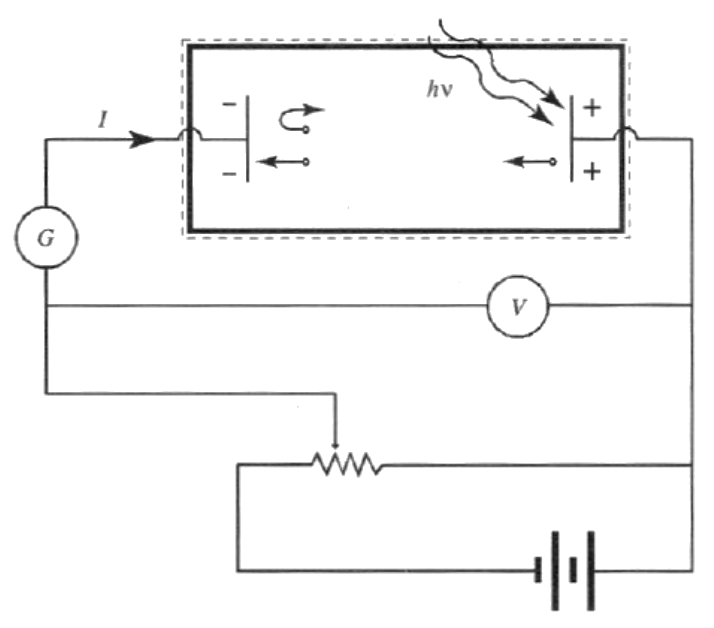
\includegraphics[width=0.45\textwidth]{Pictures/Photoelectrique.PNG}
\end{center}
\caption{\textit{Schéma de l'appareil destiné à l'étude de l'effet photoélectrique.}}
\end{figure}

On se munit d'un tube à vide contenant une électrode en Zinc. Cette dernière est éclairée par un rayon lumineux monochromatique de fréquence $\nu$. On constate que cette irradiation provoque l'émission d'électrons par la plaque de Zinc, lesquels seront collectés par une autre électrode située à l'autre extrémité du tube à vide. Les deux électrodes sont reliées entre elles par un circuit électrique muni d'un générateur de tension réglable, d'un volt-mètre et d'un ampère-mètre. 
\begin{enumerate}
\item La lumière fournit une quantité d'énergie $E$ à un électron de la plaque émettrice, convertie en travail d'extraction $W$ et énergie cinétique de l'électron libéré : $E = W + \frac{1}{2}mv^2$.
\item Lorsque l'électron est collecté par la seconde électrode, une différence de potentiel s'établit entre les deux électrodes du ``condensateur'' enfermé dans le tube à vide, ce qui crée un courant dans le circuit extérieur, mesuré par l'ampère-mètre. 
\item En outre, un générateur de tension réglable est introduit dans le circuit. Il fournit une différence de potentiel $V$ entre l'électrode émettrice et l'électrode réceptrice, appelée \textit{potentiel retardateur}.
\end{enumerate} 
$ $\\

\pagebreak

\textbf{Questions} \\
\begin{enumerate}
\item Expliquez le fait expérimental suivant : 
\begin{center}
\textit{Pour un signal lumineux de fréquence et d'intensité donnée, l'intensité du courant diminue lorsqu'on augmente le potentiel retardateur, jusqu'à atteindre 0 pour une valeur $V=V_0$ appelé \emph{potentiel d'arrêt}}.
\end{center}
Quelle quantité dynamique la mesure de $V_0$ permet-elle de déterminer ?
\item Voici un second fait expérimental.
\begin{center}
\textit{Pour une surface donnée, $V_0$ dépend de la couleur du rayonnement mais \emph{pas} de son intensité. Pour chaque métal, il existe une fréquence de seuil $\nu_s$ en-dessous de laquelle aucun courant n'est observé, et ce, quelle que soit l'intensité du rayon de lumière.}
\end{center}
Est-ce un résultat attendu, considérant la théorie ondulatoire de la lumière ?
\item Dans l'hypothèse d'Einstein, la lumière se comporte comme un flux de paquets insécables d'énergie $E=h\nu$, appelés \textit{photons}. Interprétez le résultat expérimental cité à la question précédente à la lumière de cette hypothèse.
Établissez et représentez graphiquement la relation entre $V_0$ et $\nu$, et expliquez pourquoi $\nu_s$ ne dépend que du métal employé.
\item Expérimentalement, on remarque aussi que le courant s'établit presque instantanément lorsqu'on allume le faisceau de lumière, même à très faible intensité lumineuse. Cela vous paraît-il plausible dans l'optique de la théorie ondulatoire ? Et avec l'hypothèse de quantification d'Einstein ?
\item Pour rendre plus précise la réponse à la question précédente, effectuons le petit calcul que voici. Supposons que nous éclairions (en incidence normale) une surface métallique avec une lumière d'intensité $10^{-10}\, W/m^2$. La distance moyenne entre 2 atomes du métal est de $3 \,\mathring{A}$, et chaque atome dispose d'un électron libre. L'énergie de liaison de cet électron est évaluée à $5 \, eV$. Supposons encore que la lumière est distribuée uniformément sur la surface, et que l'énergie est parfaitement absorbée par les électrons en surface. Si la radiation incidente est traitée classiquement (théorie ondulatoire), calculez le temps moyen d'irradiation qui devra s'écouler avant qu'un électron ne gagne assez d'énergie pour pouvoir être éjecté comme photo-électron ?
\end{enumerate}

\paragraph{Exercice 2} \textit{L'effet Compton.} \\
Selon la théorie quantique, un rayonnement électromagnétique monochromatique de fréquence $\nu$ peut être considéré comme un flux de photons, assimilables sous maints aspects à des particules, chacun possédant une quantité indivisible d'énergie $E=h\nu$ et une quantité de mouvement satisfaisant à la loi de De Broglie, $p = h\nu/c = h/\lambda$ ($c$ est la vitesse de la lumière dans le vide, et $\lambda$ la longueur d'onde du rayonnement). La diffusion de la lumière devient alors un problème de collision des photons avec des particules matérielles. 

\begin{figure}[h!]
\begin{center}
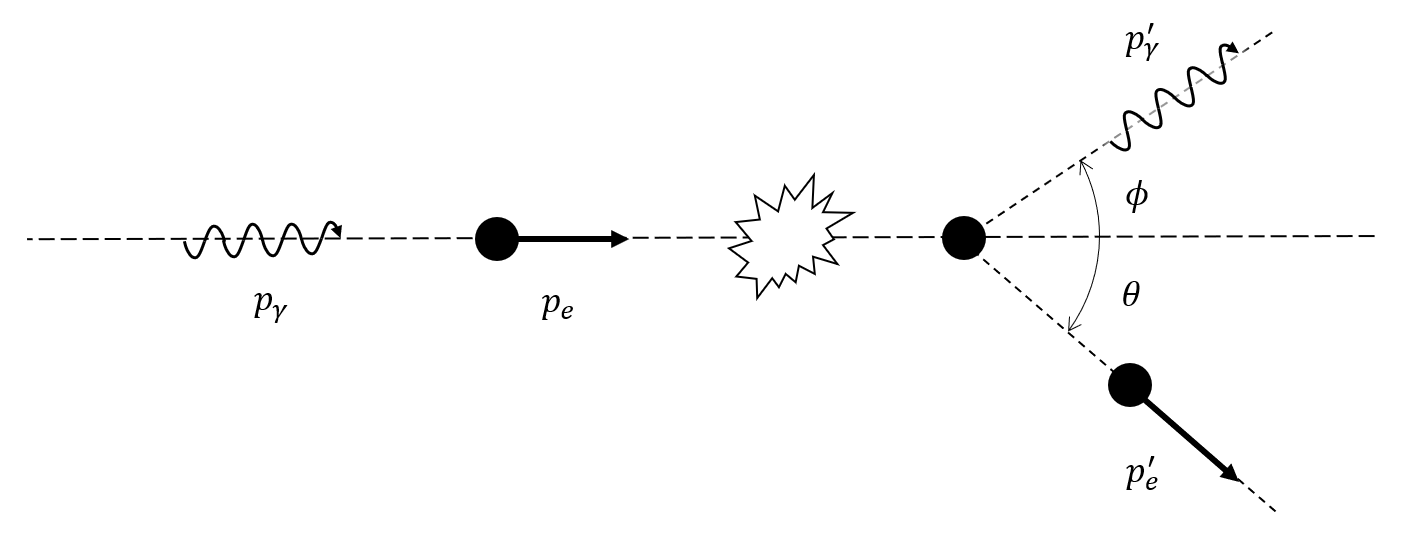
\includegraphics[width=0.75\textwidth]{Pictures/Compton.PNG}
\end{center}
\caption{\textit{Représentation schématique de la diffusion Compton.}}
\end{figure}

Supposons qu'un photon, d'impulsion $p_\gamma$, se déplace le long de l'axe $\vec{Ox}$, et rencontre un électron de quantité de mouvement $p_e$. Pour des raisons de simplicité, nous considérons que ce vecteur est aligné avec la direction de propagation du photon. Après collision, la trajectoire et la fréquence du photon sont modifiées (voir schéma pour la définition des diverses quantités). Ce phénomène, observé par Arthur Compton en 1923, acheva de convaincre les derniers sceptiques à l'égard du modèle corpusculaire de la lumière.
\begin{enumerate}
\item Écrivez la conservation de la quantité de mouvement et calculez $p'_e$.
\item Écrivez la conservation de l'énergie (relativiste) et montrez que l'énergie du photon diffusé est donnée par
\begin{equation}
E'_\gamma = \frac{E_\gamma (p_e c - E_e)}{E_\gamma (\cos\phi-1) + p_e c \cos\phi - E_e}.
\end{equation}
\item Établissez le déplacement en longueur d'onde du photon $\Delta\lambda_\gamma = \lambda_\gamma'-\lambda_\gamma$. 
\item On considère désormais que l'électron est initialement au repos. Évaluez la longueur d'onde de Compton de l'électron (pour laquelle le photon est diffusé dans la direction normale à la ligne d'incidence). Quel est le gain relatif en longueur d'onde pour de la lumière visible ($\lambda \approx 4000 \, \mathring{A}$) ? Pour du rayonnement X ($\lambda \approx 1 \, \mathring{A}$) ?
\item Calculez l'énergie transférée à l'électron en fonction de l'angle de déviation du photon. Discutez les deux régimes $E_\gamma \ll m_e c^2$ (\textit{diffusion de Thomson}) et $E_\gamma \gg m_e c^2$.
\item Montrez que $(1 + \sigma) \tan \theta = \cot (\phi/2)$ pour une constante $\sigma$ que l'on déterminera. Discutez les deux cas extrêmes $\phi=0$ et $\phi=\pi$. Pouviez-vous prévoir ce type de comportement ?
\end{enumerate}

\paragraph{Exercice 3} \textit{La diffusion de fullerènes.} \\
Les \textit{fullerènes} sont des nanoparticules formées d'un complexe de 60 atomes de carbone ($C_{60}$), et dont le nom fait référence à l'illustre architecte Buckminster Fuller (1895-1983). En 2000, elles furent utilisées par des chercheurs autrichiens pour réaliser une expérience de diffraction quantique, illustrant de manière prodigieuse la dualité onde-corpuscule pour des molécules plus complexes et massives que de simples particules élémentaires. 

\begin{figure}[h!]
\begin{center}
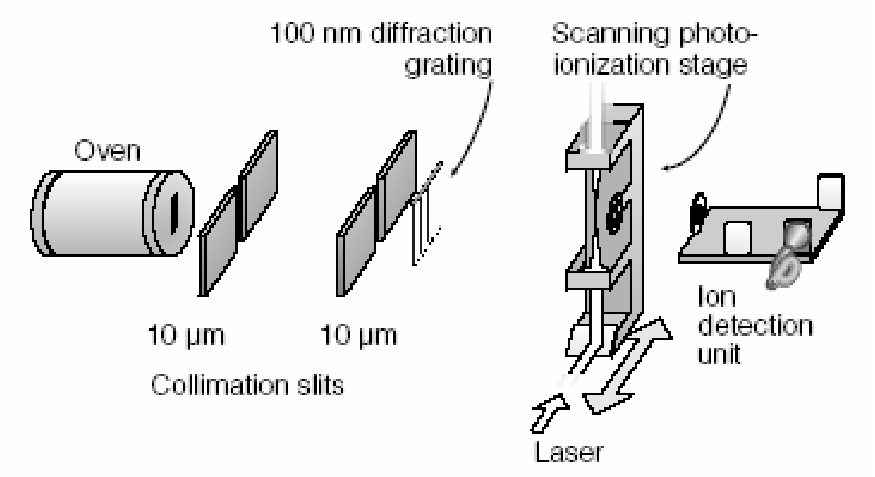
\includegraphics[width=0.55\textwidth]{Pictures/Fullerenes.PNG}
\end{center}
\caption{\textit{Dispositif expérimental. Source: [Nature \textbf{401} (2000) 691].}}
\end{figure}

\begin{enumerate}
\item Les fullerènes étaient émises par une petite ouverture dans un four chauffé à $1000 \, K$. Quelle est leur énergie cinétique, leur impulsion, leur longueur d'onde de De Broglie ?
\item Après collimation, les nanoparticules passaient à travers un réseau dont les fentes étaient espacées de $100\, nm$. Elles se propageaient ensuite sur $1.25 \, m$ avant d'être détectées. Estimez l'interfrange attendu sur la figure de diffraction. La détection s'opérait par focalisation d'un faisceau de lumière visible intense qui ionisaient les fullerènes. Les ions obtenus étaient accélérés par un champ électrique et détectés. L'interfrange est-elle compatible avec la méthode de détection utilisée ?
\end{enumerate}
Voici les résultats de l'expérience. Les deux figures reprennent les coups enregistrés dans le détecteur en fonction de la position de celui-ci, en haut, en présence du réseau, en bas, en l'absence du réseau. On remarque clairement la présence d'interférences, et leur position s'ajuste assez fidèlement aux courbes lisses en surimpression, qui représentent la figure de diffraction attendue dans une théorie purement ondulatoire de la propagation. Ceci nous indique que le comportement collectif des nanoparticules est sans conteste ondulatoire.

\begin{figure}[h!]
\begin{center}
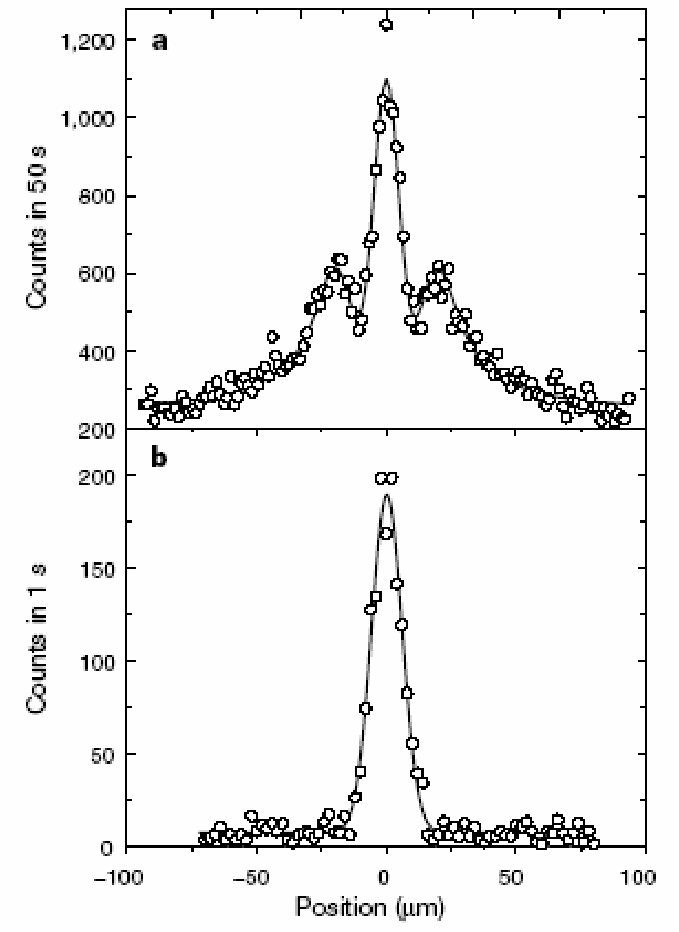
\includegraphics[width=0.55\textwidth]{Pictures/Resultat.PNG}
\end{center}
\caption{\textit{Résultats. Source: [Nature \textbf{401} (2000) 691].}}
\end{figure}
\newpage
Depuis lors, cette expérience a été répétée avec d'autres molécules plus complexes, notamment le $C_{70}$, la tetraphénylporphyrine (TPP) $C_{44} H_{30} N_4$ ou encore le fluorofullerène $C_{60} F_{48}$.

\paragraph{Exercice 4} \textit{La relation d'incertitude de Heisenberg}.
\begin{enumerate}
\item Nous désirons illustrer ici le fait que les propriétés ondulatoires de la matière ne sont pas pertinentes pour décrire le monde macroscopique. Considérons une particule d'un micromètre de diamètre, et de masse $m = 10^{-15}\, kg$. Calculez la longueur d'onde de De Broglie correspondant à cette particule si celle-ci se meut à une vitesse moyenne de $1\, mm /s$. Commentaires ?
\item Soit un virus d'une taille de $10 \, \mathring{A}$. Supposons que sa densité soit celle de l'eau, et qu'il soit confiné dans une région de largeur caractéristique approximativement égale à son diamètre moyen. Quelle est la vitesse minimale de ce virus ?
\end{enumerate}

\chapter{Équation de Schrödinger}

\paragraph{Exercice 1} \textit{Conservation des particules et courant de probabilité.} \\
On se donne une fonction d'onde $\Psi(t,\vec x)$ décrivant un système dynamique dans l'espace $\mathbb R^3$, solution de l'équation de Schrödinger 
\begin{equation}
\boxed{
-\frac{\hbar^2}{2m} \nabla^2 \Psi + V(\vec x) \Psi = i\hbar \frac{\partial\Psi}{\partial t}.
}
\end{equation}
Le module carré $|\Psi(t,\vec x)|^2$ de la fonction d'onde joue le même rôle que l'intensité pour les ondes classiques, mais doit être interprété ici comme la densité de probabilité de présence d'une particule à la position $\vec x$, à l'instant $t$. Nous allons montrer que l'équation de Schrödinger garantit la conservation de la particule au cours de son évolution. 
%Ceci suggère que lorsqu'une probabilité de présence diminue dans une région de l'espace, elle doit augmenter dans une autre, et un courant de probabilité s'est écoulé de la région que la particule quitte vers la région de destination. 
\begin{enumerate}
	\item Montrez que l'équation de Schrödinger peut se réécrire
	\begin{equation}
	\frac{\partial\rho}{\partial t} + \vec\nabla\cdot\vec J = 0
	\end{equation}
	où $\rho(t,\vec x) = |\Psi(t,\vec x)|^2$ et $\vec J(t,\vec x) = \frac{\hbar}{m} \text{Im}[\bar\Psi \vec \nabla \Psi]$. Donnez une signification physique à cette équation et aux quantités qu'elle implique. 
	\item Montrez que cela conduit à la conservation de la particule décrite par $\Psi(t,\vec x)$, et que la probabilité de présence dans l'espace complet est la norme de $\Psi(t,\vec x)$.
	%\item Sachant que l'on peut toujours écrire $\Psi(t,\vec x) = \sqrt{\rho(t,\vec x)} \, \exp i \theta(t,\vec x)$, montrez que $\vec  J(t,\vec x) = \rho(t,\vec x)\vec v(t,\vec x)$ et calculez $\vec v(t,\vec x)$. Quelle analogie vous est-elle suggérée par ce résultat ?
	%\item On se donne des champs $\rho(t,\vec x)$ et $\vec J(t,\vec x)$ arbitraires. Si l'on suppose qu'il existe un vecteur $\vec v(t,\vec x)$ tel que $\vec J = \rho\vec v$, montrez qu'il faut imposer que $\vec \nabla \times \vec v = \vec 0$ pour que l'on puisse associer la paire $(\rho,\vec J)$ à un état quantique $\Psi(t,\vec x)$. Donnez une expression générale pour le vecteur $\vec v$ en fonction de $\Psi(t,\vec x)$.
	\item On se donne des champs $\rho(t,\vec x)$ et $\vec J(t,\vec x)$ arbitraires. Montrez qu'une condition nécessaire et suffisante pour que ces champs décrivent un état physique $\Psi(t,\vec x)$ est $\vec\nabla\times (\vec J/\rho) = \vec 0$. Déduisez-en que deux états identiques peuvent différer par un facteur de phase global.
	\item Considérons une particule libre dont la quantité de mouvement $\vec p$ est \textit{parfaitement} connue. 
	\begin{enumerate}
	\item Écrivez la fonction d'onde $\Psi(t,\vec x)$ associée. 
	\item Calculez $\rho(t,\vec x)$, $J(t,\vec x)$ et interprétez vos résultats.
	\item Cette fonction d'onde est-elle de carré sommable ?
	\item Votre réponse vous surprend-elle ?
	\end{enumerate}
\end{enumerate}

\paragraph{Exercice 2} \textit{Propagation d'un paquet d'onde gaussien.} \\
Dans la réalité, la Relation de Heisenberg empêche quiconque de prédire exactement la position (respectivement l'impulsion) d'une particule sans provoquer l'indétermination totale de son impulsion (respectivement sa position). Imaginons qu'à l'origine du temps $t=0$ nous connaissions approximativement la position d'une particule autour de $x=0$, dont le mouvement sera supposé uni-dimensionnel et libre. L'incertitude sur cette position sera notée $L$. Nous pouvons représenter cette particule par une fonction d'onde gaussienne de largeur $L$ et d'impulsion initiale $p_0$ :
\begin{equation}
\Psi(0,x) = \frac{1}{\sqrt{L\sqrt{2\pi}}} e^{-\frac{x^2}{4L^2}} e^{\frac{i}{\hbar} p_0 x}.
\end{equation}	
Quelle sera la forme et la position du paquet d'onde en un instant futur $t>0$ ? C'est ce que nous allons déterminer.
\begin{enumerate}
\item Justifiez que la fonction d'onde peut généralement s'écrire comme une superposition d'ondes planes. Nous pouvons donc supposer que
\begin{equation}
\Psi(t,x) = \frac{1}{\sqrt{2\pi\hbar}} \int_{-\infty}^{+\infty} dp \, \psi(p) \, e^{\frac{i}{\hbar} (px - E(p) t)} 
\end{equation}
où les amplitudes $\psi(p)$ sont encore inconnues, et $E(p) = p^2/2m$. 
\item À l'aide de la forme de la fonction $\Psi(0,x)$, et de l'expression intégrale de la distribution de Dirac
\begin{equation}
\delta(p-p') = \frac{1}{2\pi\hbar} \int_{-\infty}^{+\infty} dx \, e^{\frac{i}{\hbar} (p-p')x},
\end{equation}
déterminez l'expression de $\psi(p)$. Calculez la moyenne statistique et l'écart-type de $\psi(p)$. Vérifiez que la Relation de Heisenberg est satisfaite.
\item Montrez que la fonction d'onde recherchée est donnée par
\begin{equation}
\Psi(t,x) = \frac{1}{(2\pi L^2 \beta^2)^{\frac{1}{4}} } e^{\frac{i}{\hbar}(p_0 x - E(p_0)t)} e^{-\frac{1}{4L^2\beta} (x - \frac{p_0}{m}t)^2}, \, \beta \equiv 1 + \frac{i\hbar t}{2mL^2}.
\end{equation}
\textit{Indication :} démontrez que
\begin{equation}
\int_{-\infty}^{+\infty} du \, e^{-\frac{u^2\alpha^2}{2}} e^{iuy} = \frac{\sqrt{2\pi}}{\alpha} e^{-\frac{y^2}{2\alpha^2}}
\end{equation}
pour $\alpha$ tel que $\text{Re}\lbrace \alpha^2\rbrace > 0$.
\item Calculez $\rho(t,x) = |\Psi(t,x)|^2$ et montrez qu'il s'agit aussi d'une distribution gaussienne, dont vous calculerez la moyenne statistique et l'écart-type. Interprétez vos résultats.
\item Calculez le courant de probabilité $J(t,x)$ associé à la propagation du paquet d'onde, et vérifiez que la particule est bien conservée.
\end{enumerate}

\paragraph{Exercice 3} \textit{Marche de potentiel.} \\
On considère une particule de masse $m$ en mouvement unidimensionnel le long de la direction $x$. Se déplaçant initialement dans la région $x<0$ de gauche à droite, elle rencontre en $x=0$ une marche de potentiel de hauteur finie et donnée par $V_0$. Nous analyserons deux cas distincts.
\begin{enumerate}
\item \textit{Réflexion partielle : $E > V_0$.} 
	\begin{enumerate}
		\item Justifiez qu'il n'existe aucun état propre d'énergie négative pour ce système.
		\item Résolvez l'équation de Schrödinger dans les régions $x>0$ et $x<0$.
		\item En guise de rafraîchissement de mémoire, montrez, comme vous l'avez vu au cours, que sous l'hypothèse d'un potentiel présentant une discontinuité finie en $x=0$ (ce qui est le cas ici !), la fonction d'onde de la particule ainsi que sa dérivée doivent être \textit{continues} en $x=0$.
		\item Faites bon usage de ces conditions de raccord pour trouver les probabilités de réflexion et transmission de la particule par la marche de potentiel. Commentez les résultats obtenus en les confrontant au cas classique.
	\end{enumerate}
\item \textit{Réflexion totale : $E < V_0$.}
	\begin{enumerate}
		\item Résolvez l'équation de Schrödinger dans les régions $x>0$ et $x<0$.
		\item Exigez la continuité de la fonction d'onde et de sa dérivée pour trouver les probabilités de réflexion et transmission de la particule par la marche de potentiel. 
		\item Supposons que vous soyez en mesure de photographier le système à un instant arbitrairement choisi. Est-il possible que la particule soit photographiée à \textit{droite} de la marche de potentiel ? Commentez.
		\item Calculez le déphasage entre l'onde incidente et l'onde réfléchie, et donnez-en une interprétation physique.
	\end{enumerate}
\end{enumerate}

\paragraph{Exercice 4} \textit{État lié dans un puits de potentiel infiniment mince.} \\
On considère une particule de masse $m$ en mouvement unidimensionnel le long de la direction $x$ et dont l'opérateur Hamiltonien est donné par
\begin{equation}
H = -\frac{\hbar^2}{2m} \frac{d^2}{dx^2} - \alpha \delta(x)
\end{equation}
où $\alpha$ est une constante réelle positive dont on donnera les dimensions.
\begin{enumerate}
\item Formez l'équation de Schrödinger qui décrit le mouvement de la particule. 
\item Intégrez-la autour du point ``dramatique'' $x=0$ sur un intervalle de rayon $\varepsilon >0$ quelconque fixé et arbitrairement proche de zéro. Montrez que la dérivée de la fonction d'onde $\Psi(x)$ subit une discontinuité en $x=0$ que vous exprimerez en fonction de $\alpha$, $m$ et $\Psi(0)$.
\item On suppose que l'énergie $E$ de la particule est négative (état lié). Résolvez l'équation de Schrödinger dans les régions $x<0$ et $x>0$.
%\begin{equation}
%\left\lbrace
%\begin{array}{ccc}
%x<0 & : & \Psi(x) = A_1 e^{\rho x} + A_1' e^{-\rho x} \\ 
%x>0 & : & \Psi(x) = A_2 e^{\rho x} + A_2' e^{-\rho x}
%\end{array} 
%\right.
%\end{equation}
%Déterminez la constante $\rho$ en fonction de $E$ et $m$.
\item Exigez les conditions de raccord en $x=0$ pour fixer les valeurs possibles pour l'énergie $E$, ainsi que les fonctions d'onde normées correspondantes.
\item Représentez graphiquement les fonctions d'onde déterminées au point précédent, et donnez un ordre de grandeur de leur largeur $\Delta x$. 
\end{enumerate}

\paragraph{Exercice 5} \textit{Transmission à travers une barrière de potentiel infiniment mince.} \\
On considère une particule de masse $m$ en mouvement unidimensionnel le long de la direction $x$ et dont l'opérateur Hamiltonien est à nouveau donné par
\begin{equation}
H = -\frac{\hbar^2}{2m} \frac{d^2}{dx^2} - \alpha \delta(x).
\end{equation}
On suppose qu'elle se propage de gauche à droite le long de la direction $x$ avec une énergie $E$ positive. 
\begin{enumerate}
\item Montrez qu'un état stationnaire de la particule peut s'écrire :
\begin{equation}
\left\lbrace
\begin{array}{ccl}
x<0 & : & \Psi(x) = e^{ikx} + A \, e^{-ikx} \\ 
x>0 & : & \Psi(x) = B \, e^{ikx}
\end{array} 
\right.
\end{equation}
où $k$, $A$ et $B$ sont des constantes dont vous calculerez la valeur en fonction de $E$, $m$ et $\alpha$. 
\item Posons $-E_L \equiv -m\alpha^2/2\hbar^2$, l'énergie de l'état lié de la particule. Calculez, en fonction du paramètre sans dimensions $\sigma = E/E_L$ les coefficients de réflexion et transmission de la barrière, notés respectivement $\mathcal{R}$ et $\mathcal{T}$.
\item Décrivez la variation de $\mathcal{R}$ et $\mathcal{T}$ en fonction de l'énergie incidente $E$. Que se passe-t-il lorsque $E\to+\infty$ ? Commentaires ?
\item Montrez que, si l'on prolonge l'expression de $\mathcal{T}$ pour des valeurs d'énergie négatives, elle diverge lorsque $E\to-E_L$. Commentaires ?
\end{enumerate}

\paragraph{Exercice 6} \textit{Piège quantique à murs infiniment minces.} \\
On considère une particule de masse $m$ en mouvement unidimensionnel le long de la direction $x$, dont l'énergie potentielle s'écrit
\begin{equation}
V(x) = -\alpha \delta(x)-\alpha \delta(x-\ell), \, \alpha>0,\, \ell >0.
\end{equation}
\begin{enumerate}
\item Calculez les états liés de la particule en fonction du paramètre $\rho$ défini implicitement par 
\begin{equation}
E = -\frac{\hbar^2\rho^2}{2m}.
\end{equation}
Montrez que les niveaux d'énergie possibles vérifient la relation
\begin{equation}
e^{-\rho\ell} = \pm \Big( 1 - \frac{2\rho}{\mu} \Big), \,\mu = \frac{2m\alpha}{\hbar^2}.
\end{equation}
Donnez une résolution graphique de cette équation.
\item Décrivez les états stationnaires du système.
	\begin{enumerate}
	\item \textit{État fondamental.} Montrez que l'état fondamental est pair, c'est-à-dire invariant par symétrie miroir par rapport au point central $x=\ell/2$. Montrez que son énergie $E_S$ est inférieure à l'énergie $-E_L$ de l'état lié introduite à l'exercice précédent. Donnez une interprétation physique pour ce résultat. Représentez graphiquement la fonction d'onde correspondante.
	\item \textit{État excité.} Montrez que, lorsque le puits est suffisamment large (au-delà d'une valeur critique pour $\ell$ que vous calculerez), il existe un état excité, impair cette fois, et d'énergie $E_A$ supérieure à $-E_L$. À nouveau, interprétez et représentez graphiquement la fonction d'onde correspondante.
	\end{enumerate}
\end{enumerate}

\paragraph{Exercice 7} \textit{Mouvement circulaire uniforme --- Modèle de Bohr.}  \\
Considérons une particule de masse $m$ confinée sur un cercle de rayon $R$ et de circonférence $L = 2\pi R$. Plus précisément, on admet qu'un potentiel confine la particule dans les directions transverses. Ce potentiel est tellement fort qu'aux échelles d'énergie que nous envisageons, le seul degré de liberté est le mouvement le long du cercle.\\

\begin{center}
    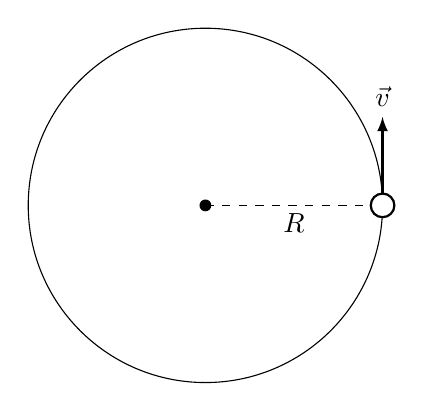
\begin{tikzpicture}[scale=0.75]
    \draw (2,2) circle (3cm);
    \fill (2,2) circle (0.1cm);
    \draw[dashed] (2,2) -- (5,2);
    \draw[-latex,thick] (5,2) -- (5,3.5)node[above]{$\vec v$};
    \draw[thick,fill=white] (5,2) circle (0.2cm);
    \node at (3.5,1.7) {$R$};
    \end{tikzpicture}
\end{center}
$ $\\
Soit $x \in [-\frac{L}{2},\frac{L}{2}]$ la coordonnée le long du cercle. L'origine $x=0$ est arbitrairement choisie, puisque ce système possède une symétrie de rotation.

\begin{enumerate}
    \item Quelles sont les conditions de raccord en $x= \pm \frac{L}{2}$ qu'il faut imposer sur $\psi(x)$ pour respecter la symétrie du problème ?
    \item Démontrez que les niveaux d'énergie de la particule sont quantifiés $\lbrace E_n\rbrace_{n\in\mathbb N}$, et déterminez les fonctions d'onde $\lbrace \varphi_n(x)\rbrace_{n\in\mathbb N}$ correspondantes. Les états sont-ils dégénérés ?
    \item Montrez que les fonctions d'onde associées à $m\neq n$ sont mutuellement orthogonales.
    \item Démontrez que le moment cinétique orbital de la particule est quantifié, $\mathcal L_n = \hbar n$.
    \end{enumerate}
    Le résultat précédent est en fait assez fondamental : le \textit{modèle de Bohr} de l'atome d'Hydrogène peut d'ailleurs être construit à partir de ce principe. Considérons un électron décrivant une orbite circulaire \textit{supposée} stable dans le potentiel électrostatique d'un proton, et faisons l'hypothèse que son moment cinétique orbital vérifie $\mathcal L = \hbar n$ où $n\in \mathbb N_0$. 
    \begin{enumerate}
    \setcounter{enumi}{4}
    \item Montrez que le rayon de cette orbite vérifie $R_n = a_0 n^2$ où $n\in\mathbb N_0$ et $a_0$ est le rayon de Bohr que l'on calculera. Comment pouviez-vous estimer la valeur de $a_0$ ?
    \item Quels sont, dans ce modèle, les niveaux d'énergie $\varepsilon_n$ de l'atome d'Hydrogène ? 
    \item Calculez la longueur d'onde dans le vide de la raie correspondant à la transition d'un électron du niveau $n'$ vers le niveau $n$ de l'atome d'Hydrogène (\textit{formule de Rydberg}). Quelle est l'énergie d'ionisation de cet atome ? 
\end{enumerate}

\newpage

\paragraph{Exercice 8} \textit{Boîte quantique avec barrière infiniment mince.} \hfill [\textit{Septembre 2019}] \\

Considérons une particule de masse $m$ confinée entre $x= -\frac{L}{2}$ et $x =+\frac{L}{2}$. En $x=0$ se trouve une barrière de potentiel suffisamment mince pour que nous puissions la représenter par une distribution $\delta$. \\

L'équation de Schrödinger stationnaire pour la particule est donc
\begin{equation}
-\frac{\hbar^2}{2m} \frac{d^2}{d x^2} \psi(x) + \alpha\, \delta(x)\, \psi(x)= E\, \psi(x)
\label{Eq:SchrDelta}
\end{equation}
avec $\alpha>0$ et les conditions aux bords $\psi(-\frac{L}{2})=0=\psi(+\frac{L}{2})$.

\begin{enumerate}
\item Quels sont les états stationnaires du système lorsque $\alpha = 0$. Calculez les niveaux d'énergie correspondants.

\item Dorénavant, nous considérons $\alpha \neq  0$. Quelles conditions de raccord faut-il imposer en $x=0$ pour tenir compte du potentiel $\delta$ ?

\item
Démontrez que toute solution de l'équation  \eqref{Eq:SchrDelta} possède une parité bien définie. Montrez en particulier que les fonctions d'onde impaires, solutions de l'équation \eqref{Eq:SchrDelta} avec $\alpha=0$ (trouvées au point 1), sont également solutions lorsque $\alpha\neq 0$ avec la même énergie.

\item Considérons à présent les solutions paires. En utilisant la condition de raccord dérivée au point 2, déterminez les niveaux d'énergie de ces solutions. 

\textit{Note :} Ces niveaux d'énergie seront donnés par une équation transcendante que vous ne pourrez pas résoudre analytiquement !
\end{enumerate}

\begin{figure}[h!]
    \centering
    \begin{tikzpicture}[scale=0.75]
    \draw[->] (-6,0) -- (6,0) node[right]{$x$};
    \draw[->] (-6,0) -- (-6,5) node[above]{$V$};
    \draw[very thick]  (-4,6) -- (-4,0);
    \draw  (-0.1, 4) -- (-0.1,0);
    \draw  (-0.1, 4) -- (0.1,4);
    \draw  (0.1, 4) -- (0.1,0);
    \draw[very thick]  (4,6) -- (4,0);
    %\node at (6,-0.5) {$x$};
    %\node at (-6.5,5) {$V$};
    \node at (-4,-0.5) {$-\frac{L}{2}$};
    \node at (0,-0.5) {$0$};
    \node at (4,-0.5) {$+\frac{L}{2}$};
    \node[above] at (0,4) {$\uparrow$};
    \node[above] at (0,4.6) {$\infty$};
    \fill[pattern=north east lines, pattern color=black] (4,0) rectangle (4.25,6);
    \fill[pattern=north west lines, pattern color=black] (-4,0) rectangle (-4.25,6);
    \end{tikzpicture}
    \caption{Représentation schématique du potentiel $V(x)$ de l'équation \eqref{Eq:SchrDelta}: $V$ est infini pour $x<-\frac{L}{2}$ et pour $x>\frac{L}{2}$. En outre un potentiel $\delta$ est présent en $x=0$.}
\end{figure}

\paragraph{Questions d'examen:} Juin 2019 Q4, Août 2019 Q4, Juin 2021 Q3, Août 2022 Q3.

\chapter{Formalisme de Dirac}

\textit{Conventions.} Nous travaillons avec des espaces de Hilbert $\mathcal H$ dont les vecteurs sont représentés par les \textit{kets} $\ket{\psi}$. Les formes linéaires sur ces espaces sont écrites sous forme de \textit{bras} $\bra{\psi}$, de sorte que le produit scalaire dans $\mathcal H$ sera noté $\braket{\phi}{\psi}$, avec la notation \textit{braket} qui incorpore directement le théorème de représentation de Riesz. Les opérateurs agissant dans $\mathcal H$ seront toujours repérés par un accent circonflexe, $\hat A$, alors que les matrices qui les représentent dans une base donnée en seront dépourvues, $A$. Parmi les opérateurs, on comptera en particulier les produits dyadiques, représentés par $\ket{\psi}\bra{\phi}$, ainsi que l'identité, notée $\hat I$.\\
$ $

\paragraph{Exercice 1} \textit{Découverte du formalisme de Dirac.}
\begin{enumerate}
\item L'espace des états d'un système physique $S$ est à deux dimensions. Soit $\mathscr B = \lbrace \ket{\phi_1},\ket{\phi_2}\rbrace$ une base orthonormée de cet espace. On définit les \textit{kets} $\ket{\psi}$ et $\ket{\chi}$ par :
	\begin{equation}
	\ket{\psi} = 9i\ket{\phi_1} + 2 \ket{\phi_2} \quad ; \quad \ket{\chi} = \frac{1}{\sqrt{2}} \ket{\phi_1} -\frac{i}{\sqrt{2}} \ket{\phi_2}.
	\end{equation}
	
\begin{enumerate}
\item Calculez les produits scalaires $\braket{\psi}{\psi}$, $\braket{\chi}{\chi}$, $\braket{\psi}{\chi}$ et $\braket{\chi}{\psi}$. Déduisez-en la valeur du produit scalaire $\braket{\psi+\chi}{\psi+\chi}$. Les quantités $\braket{\psi}{\chi}$ et $\braket{\chi}{\psi}$ sont-elles égales ?
\item Formez les opérateurs $\hat A = \ketbra{\psi}{\chi}$ et $\hat B = \ketbra{\chi}{\psi}$, sont-ils égaux ? Calculez leur trace, qu'observez-vous ?
\item Établissez l'expression des opérateurs réalisant la projection orthogonale le long de $\ket{\psi}$ et $\ket{\chi}$ respectivement. Calculez leur trace. 
\item On définit les vecteurs $\ket{\pm} = N(\ket{\phi_1}\pm\ket{\phi_2})$, où $N$ est une constante de normalisation à déterminer. Calculez les opérateurs de projection orthogonale sur ces vecteurs. Sont-ils hermitiens ? Montrez que leurs ensembles images sont orthogonaux. Calculez leur somme. Commentaires ?
\item Montrez que $\ket{+}$ et $\ket{-}$ forment une nouvelle base $\mathscr B'$ orthonormale de $S$ et donnez la matrice de changement de base.
\item Dans la base $\mathscr B$, un opérateur $\hat H$ est représenté par la matrice
\begin{equation}
H = \left[
\begin{array}{cc}
1 & \alpha \\
\alpha & 1
\end{array}
\right], \,\,\alpha\in\mathbb R_0.
\end{equation}
Déterminez la représentation de $\hat H$ dans la nouvelle base $\mathscr B'$, d'une part en utilisant la procédure algébrique habituelle, et d'autre part, en se reposant uniquement sur la notation de Dirac. 
\end{enumerate}

\item Soit un espace de Hilbert $\mathscr H$ sur lequel agit l'opérateur $\hat H = \alpha \ketbra{\phi_1}{\phi_2} + h.c.$ où $\alpha\in\mathbb R_0$, et les $\ket{\phi_i}$ sont les vecteurs propres normalisés, et non-dégénérés, d'un opérateur $\hat A$ auto-adjoint pour le produit scalaire dont $\mathscr H$ est muni.
\begin{enumerate}
\item Déterminez $p,q\in\mathbb Z_0$ tels que $\hat P = \alpha^p \hat H^q$ soit un projecteur. Déterminez $\text{Ker}\,\hat P$ et $\text{Im}\, \hat P$. Commentaires ?
\item Calculez le commutateur $[\hat H,\ketbra{\phi_1}{\phi_1}]$. Pouvez-vous en déduire $[\hat H,\ketbra{\phi_2}{\phi_2}]$ ?
\item Sans construire explicitement la matrice de $\hat H$, trouvez les vecteurs propres de $\hat H$ ainsi que les valeurs propres correspondantes.
\item Construisez la matrice représentant $\hat H$ dans la base que vous avez à votre disposition. Vérifiez alors vos résultats obtenus du point précédent.
\end{enumerate}

\end{enumerate}

	
\paragraph{Exercice 2} \textit{Base d'opérateurs.} \\
Soit un espace de Hilbert de dimension $N\in\mathbb N_0$. On imagine qu'il existe un opérateur $\hat H$ agissant dans cet espace, qui soit hermitien et possède un ensemble de vecteurs propres non-dégénérés notés $\lbrace\ket{\varphi_n}\rbrace$. Pour les besoins de l'exercice, nous supposerons que ces vecteurs de base sont normés : $\braket{\varphi_n}{\varphi_n} = 1$, $\forall n$. 
\begin{enumerate}
	\item Justifiez que $\mathscr B = \lbrace\ket{\varphi_n}\rbrace_{n\in\mathbb{N}}$ constitue une base orthonormée de l'espace de Hilbert. 
	\item Pour tout couple de naturels $(m,n)$, on définit l'opérateur $\hat U(m,n) = \ket{\varphi_m}\bra{\varphi_n}$. Interprétez l'action de $\hat U(m,n)$ lorsque $m\neq n$.
	\item Quel sens donnez-vous à $\hat U(n,n)$ ? Montrez qu'il faut et il suffit que $\sum_{n=1}^N \hat U(n,n) = \hat I$ pour que $\mathscr B$ forme une base orthonormée de l'espace de Hilbert (\textit{relation de fermeture}).
	\item Calculez l'adjoint de $\hat U(m,n)$ ainsi que le commutateur $[\hat H,\hat U(m,n)]$.
	\item Calculez $\hat U(m,n) \hat U^\dagger (p,q)$, $\forall\, m,n,p,q \in \mathbb{N}_0$, ainsi que $\text{tr} [\hat U(m,n)]$. 
	\item Soit un opérateur $\hat A$ dont les éléments de matrice dans la base $\mathscr B$ sont les nombres complexes $A_{mn}$. Démontrez la relation $\hat A = \sum_{m,n} A_{mn} \hat U(m,n)$.
	\item Prouvez que si l'on dispose de l'opérateur $\hat A$ et de la collection d'opérateurs $\hat U(m,n)$, on peut facilement obtenir les composantes $A_{mn}$ en calculant $A_{mn} = \text{tr} [\hat A \hat U^\dagger (m,n)]$. Quel sens donnez-vous alors à $\hat U(m,n)$ ?
\end{enumerate}
	
\paragraph{Exercice 3} \textit{Structures propres (2 dimensions).} \\
Soit un opérateur hermitien $\hat A$ agissant dans un espace de Hilbert à 2 dimensions dont on considère la base orthonormée $\lbrace \ket{1},\ket{2}\rbrace$. Nous dénoterons par $A_{mn}$ l'élément de matrice $\langle m|\hat A|n\rangle$.
\begin{enumerate}
\item Montrez qu'il existe un opérateur hermitien $\hat A'$, sans dimensions et sans trace, tel que $\hat A = \frac{1}{2}\alpha\hat I+\frac{1}{2}\beta\hat A'$, avec $\alpha = \text{Tr}\hat A$. Donnez l'expression de $\beta$ et des $A'_{mn}$ en termes des $A_{mn}$.
\item On définit les angles $\theta\in[0,\pi]$ et $\phi\in[0,2\pi[$ par $\theta = \text{arctan}\left[\frac{2|A_{21}|}{A_{11}-A_{22}}\right]$ et $\phi = \text{arg}(A_{21})$. Déterminez la structure propre de $\hat A'$ en fonction de $(\theta,\phi)$.
\item Déduisez-en les valeurs et vecteurs propres de $\hat A$ en fonction de $(\theta,\phi)$. Commentaires ?
\item À quelle condition le spectre de $\hat A$ est-il dégénéré ?
\end{enumerate}

\paragraph{Exercice 4} \textit{Structures propres (3 dimensions).} \\
Soient deux transformations linéaires $\hat A,\hat B : \mathbb{R}^3 \to \mathbb{R}^3$ dont les matrices exprimées par rapport à la base canonique $\mathscr B$ de $\mathbb{R}^3$ sont
\begin{equation}
A = \left[ \begin{array}{ccc}
0 & 1 & 0 \\ 
1 & 0 & 1 \\ 
0 & 1 & 0
\end{array} \right] \quad ; \quad
B = \left[ \begin{array}{ccc}
1 & 2 & 0 \\ 
2 & -1 & -2 \\ 
0 & -2 & 1
\end{array} \right].
\end{equation}
\begin{enumerate}
\item Caractérisez l'opérateur $\hat A$, ainsi que son spectre. Est-il diagonalisable ? Donnez son expression dans la base canonique de $\mathbb R^{3\times 3}$. Mêmes questions pour $B$.
\item Déterminez les valeurs propres, ainsi que les vecteurs propres normalisés de $\hat A$ et $\hat B$. 
\item Montrez que les vecteurs propres de $\hat A$ forment une nouvelle base orthonormée complète $\mathscr B'$ par rapport au produit scalaire $\braket{\vec x}{\vec y} = \sum_i x_i y_i$ dans $\mathbb R^3$, et justifiez-le. 
\item Calculez les matrices de projection sur les sous-espaces propres de $\hat A$. Vérifiez que ces projeteurs satisfont à des relations d'orthogonalité et de complétude. Interprétez cet état de fait.
\item Déterminez et caractérisez l'opérateur $\hat U$ qui permet, par transformation de similitude, d'obtenir la forme de Jordan de $\hat A$, et donnez sa matrice dans les bases $\mathscr B$ et $\mathscr B'$.
\item Calculez les matrices représentant $\hat A$ et $\hat B$ dans la base $\mathscr B'$ de deux façons différentes.
\end{enumerate}
\textit{Pour s'entraîner} : analysez la structure propre des opérateurs décrits par les matrices suivantes
\[
\left[
\begin{array}{ccc}
7 & 0 & 0 \\ 
0 & 1 & -i \\ 
0 & i & -1
\end{array} 
\right], \,
\left[
\begin{array}{ccc}
0 & 1 & 2 \\ 
1 &2 & 0 \\ 
2 & 0 & 1
\end{array} 
\right], \,
\left[
\begin{array}{ccc}
0 & -i & i \\ 
-i & 0 & i \\ 
i & i & 0
\end{array} 
\right], \,
\left[
\begin{array}{ccc}
0 & -6 & -4 \\ 
5 & -11 & -6 \\ 
-6 & 9 & 4
\end{array} 
\right].
\]
$ $


	
\paragraph{Exercice 5} \textit{Projecteurs orthogonaux.}\\ 
Il existe une classe bien utile d'opérateurs qui réalisent une projection sur un sous-espace qui soit orthogonal à son complémentaire. Cet exercice se fixe pour but de donner une caractérisation de ces projecteurs, dits \textit{orthogonaux}, ainsi que d'étudier leur composition.
\begin{enumerate}
\item Montrez que si $\hat P$ est un projecteur, alors $ \hat I - \hat P$ est également un projecteur, et déterminez les sous-espaces $\text{Ker}(\hat I - \hat P)$ et $\text{Im}(\hat I - \hat P)$.
\item Démontrez qu'un projecteur $\hat P$ est orthogonal si et seulement si $\hat P = \hat P^\dagger$.
\end{enumerate}
Soient $\hat P_1$ le projecteur orthogonal sur le sous-espace vectoriel $\mathcal{E} _1$ de l'espace vectoriel $\mathcal{V}$, et $\hat P_2$ le projecteur orthogonal sur le sous-espace vectoriel $\mathcal{E}_2$.
\begin{enumerate}
\setcounter{enumi}{2}
\item Montrez que le produit $\hat P_1\hat P_2$ est un projecteur orthogonal si et seulement si $\hat P_1$ et $\hat P_2$ commutent. Si tel est le cas, quel est le sous-espace sur lequel projette $\hat P_1\hat P_2$ ?
\item  Montrez que la somme $\hat P_1+\hat P_2$ est un projecteur orthogonal si et seulement si $\hat P_1\hat P_2$ est zéro. Dans ce cas, déterminez le sous-espace sur lequel projette $\hat P_1+\hat P_2$.
\item Montrez que $\hat P_1 +\hat P_2 - \hat P_1\hat P_2$ est un projecteur orthogonal à condition que $\hat P_1$ et $\hat P_2$ commutent. Sur quel sous-espace cet opérateur projette-t-il ?
\end{enumerate}


\paragraph{Exercice 6} \textit{Opérateurs unitaires.} \\
Nous savons désormais que les valeurs propres d'un opérateur hermitien sont réelles, et que les vecteurs propres associés à des valeurs propres distinctes sont orthogonaux. Nous allons prouver que les opérateurs unitaires, d'importance primordiale pour la Mécanique Quantique, jouissent de propriétés similaires.
\begin{enumerate}
\item Soit $\hat U$ un opérateur unitaire, $\hat U \hat U^\dagger = \hat U^\dagger \hat U = \hat I$. Montrez que les valeurs propres de $\hat U$ sont des nombres complexes de module $1$. 
\item Montrez que les vecteurs propres de $\hat U$ associés à des valeurs propres \textit{distinctes} sont orthogonaux. 
\end{enumerate}

\paragraph{Exercice 7} \textit{Fonctions de matrices et d'opérateurs.} \\
Soit $f(x)$ une fonction analytique d'une variable complexe. 
\begin{enumerate}
\item Pour une matrice $A$ à coefficients complexes, comment donner sens à $f(A)$ ?
\item Soit $D$ une matrice diagonale. Calculez explicitement $f(D)$.
\item Soient $M$ et $N$ deux matrices semblables. Montrez que $f(M)$ et $f(N)$ sont également semblables et donnez la transformation de similitude.
\item Utilisez les résultats précédents pour expliciter $f(H)$ où $H$ est une matrice hermitienne.
\newpage
\item Concentrons-nous à présent sur les transformations de $\mathbb R^n$, où $n\in\mathbb N_0$. 
\begin{enumerate}
\item Soit $A$, une matrice de $\mathbb R^{n\times n}$. Définissez l'exponentielle matricielle $e^A$ et montrez qu'elle existe toujours.
\item Montrez que $B = e^A$ est inversible, et donnez $B^{-1}$.
\item Prouvez que $B$ est une transformation orthogonale si $A$ est antisymétrique.
\end{enumerate}
\item Particularisons maintenant aux transformations de l'espace euclidien $\mathbb R^3$, dont la base canonique est notée $\mathscr B = \lbrace \vec e_x,\vec e_y,\vec e_z \rbrace$. Considérons les 3 matrices suivantes, exprimées dans $\mathscr B$ :
\begin{equation}
L_x = \left[
\begin{array}{ccc}
0 & 0 & 0 \\ 
0 & 0 & -1 \\ 
0 & 1 & 0
\end{array} 
\right], \quad
L_y = \left[
\begin{array}{ccc}
0 & 0 & 1 \\ 
0 & 0 & 0 \\ 
-1 & 0 & 0
\end{array} 
\right], \quad
L_z = \left[
\begin{array}{ccc}
0 & -1 & 0 \\ 
1 & 0 & 0 \\ 
0 & 0 & 0
\end{array} 
\right].
\end{equation}
\begin{enumerate}
\item Calculez $R_a (\theta) \equiv e^{\theta L_a}$ avec $a = x,y,z$ paramétrées par $\theta\in [0,2\pi[$.
\item Que représentent les trois transformations linéaires dont les $R_a$ sont les matrices dans la base canonique $\mathscr B$ ?
\item Calculez les matrices représentant des transformations \textit{infinitésimales} $R_a (\delta \theta)$ où le paramètre $\delta\theta \ll 1$. Déduisez-en le rôle des $L_a$.
\item Calculez les commutateurs $[L_a,L_b] = L_aL_b-L_bL_a$, $\forall a,b \in \lbrace x,y,z \rbrace$. Commentaires ?
\end{enumerate}
\end{enumerate}


\paragraph{Exercice 8} \textit{Propriétés des commutateurs.} \\
Très souvent, nous allons essayer d’analyser les propriétés de systèmes physiques en regardant de plus près les propriétés des opérateurs qui agissent sur ce système. En particulier, on va très fréquemment s'intéresser aux propriétés des commutateurs de ces opérateurs, lesquels sont les analogues quantiques des crochets de Poisson classiques, par le truchement du Principe de Correspondance. Voici donc quelques exercices qui permettent de revoir ou de découvrir quelques propriétés très utiles du commutateur de deux opérateurs $[\hat A,\hat B] = \hat A\hat B-\hat B\hat A$.
\begin{enumerate}
\item Considérons trois opérateurs $\hat A$, $\hat B$ et $\hat C$. Prouvez les assertions suivantes :
	\begin{enumerate}
	\item Le commutateur est bilinéaire, antisymétrique et vérifie l'\textit{identité de Jacobi}\\ $[[\hat A,\hat B],\hat C] + [[\hat C,\hat A],\hat B] + [[\hat B,\hat C],\hat A] = 0$.
	\item Le commutateur se distribue sur le produit $[\hat A,\hat B\hat C] = [\hat A,\hat B]\hat C + \hat B [\hat A, \hat C]$.
	\end{enumerate}
\item Supposez que $\hat A$ et $\hat B$ commutent avec leur commutateur $[\hat A,\hat B]$. Prouvez alors que $[\hat A,\hat B^n] = n \hat B^{n-1} [\hat A, \hat B]$ et $[ \hat A^n, \hat B] = n  \hat A^{n-1} [ \hat A, \hat B]$ ,$\forall n \in \mathbb{N}$.
\item Généralisez le résultat précédent en montrant, pour toute fonction analytique $F( \hat B)$, que $[ \hat A,F( \hat B)] = [ \hat A, \hat B] F'( \hat B)$. 
\item Démontrez qu'à condition que $\hat  A$ et $\hat  B$ commutent avec leur commutateur, on a
\begin{equation}
\exp(\hat  A) \exp(\hat  B) = \exp(\hat  A + \hat  B) \exp([\hat  A,\hat  B]/2).
\end{equation}
C'est un cas particulier de l'\textit{identité de Baker-Hausdorff}.
\end{enumerate}
	
\paragraph{Exercice 9} \textit{Espace métrique de fonctions.} \\
Soit $\mathcal W = \mathcal P_3([-1,1])$, l'ensemble des polynômes de degré au plus 3 définis sur l'intervalle $[-1,1]$ de la droite réelle, sur lequel on peut définir le produit scalaire
\begin{equation}
\langle \cdot|\cdot\rangle : \mathcal W \times \mathcal W\to\mathbb R : (f,g) \mapsto \langle f|g\rangle = \int_{-1}^{+1} dx\, f(x)g(x).
\end{equation}
\begin{enumerate}
\item Montrez que $\mathcal W$ est un espace vectoriel de dimension $4$ dont la base canonique est $\lbrace 1,x,x^2,x^3 \rbrace$. On notera cette base $\mathscr B = \lbrace \ket 0,\ket 1,\ket 2,\ket 3\rbrace$. 
\item Déterminez l'expression de l'opérateur $\hat D : \mathcal W\to \mathcal W : f(x) \mapsto f'(x)$ dans la base canonique.
\item Exprimez de même l'opération de translation $\hat T_a : \mathcal W \to \mathcal W : f(x) \mapsto f(x+a)$, où $a$ est un nombre réel arbitrairement fixé.
\item Montrez que $\hat T_a = \exp a \hat D$. En considérant la limite $a\ll 1$, interprétez le rôle de $\hat D$. Quel célèbre résultat retrouvez-vous ?
\item Déterminez une base orthonormée de l'espace $\mathcal W$, notée $\lbrace \ket{P_n}\rbrace_{n=0}^3$. Écrivez votre résultat explicitement en termes de la coordonnée $x$ : vous obtenez ainsi les 4 premiers polynômes de Legendre !
\item Considérez l'opérateur $\hat A = \hat D \circ [(1-x^2)\hat D]$. Montrez que $\hat A^\dagger = \hat A$.
\item Calculez la matrice de $\hat A$ dans la base des polynômes de Legendre, qu'observez-vous ?
\end{enumerate}


\chapter{Postulats \& applications}

\paragraph{Exercice 1} \textit{Évolution quantique.}\\
Soit un système quantique dont l'état dépendant du temps est noté $\ket{\psi(t)}$, et dont l'opérateur Hamiltonien s'écrit $\hat H(t)$. 
\begin{enumerate}
\item \textbf{Opérateur d'évolution.}
\begin{enumerate}
\item Déduisez de l'uniformité du temps de la Relativité Galiléenne qu'il existe un opérateur unitaire $\hat U(t,t_0)$ qui fasse évoluer l'état $\ket{\psi(t)}$ du temps $t_0$ de référence au temps $t\geq t_0$. 
\item Prouvez que cet $\hat U(t,t_0)$ est unique, et ne dépend donc pas de l'état de départ $\ket{\psi(t_0)}$.
\item Montrez que l'ensemble de tels opérateurs $\hat U(t,t_0)$ doit former un groupe à un paramètre pour la loi de composition des opérateurs agissant sur l'espace des états du système.
\end{enumerate} 
\item \textbf{Évolution des états quantiques.}
\begin{enumerate}
\item Montrez que l'équation d'évolution d'un état quantique $\ket{\psi(t)}$ est de la forme 
\begin{equation}
i\hbar \frac{\partial}{\partial t}\ket{\psi(t)} = \hat A(t,t_0)\ket{\psi(t)}
\end{equation}
pour un opérateur $\hat A(t,t_0)$ que l'on calculera en fonction de $\hat U(t,t_0)$.
\item Démontrez que $\hat A(t,t_0)$ est hermitien et indépendant de $t_0$. On notera donc $\hat A(t)$.
\item Justifiez, grâce au Principe de Correspondance \textit{et} la définition de $\hat H$ que $\hat A(t) = \hat H(t)$ est un choix physiquement raisonnable. Qu'avez-vous retrouvé ?
\item Donnez l'expression de $\hat U(t,t_0)$ pour un système conservatif (le cas général fait l'objet d'un calcul assez technique qui ne sera pas abordé ici). 
\item Pouvez-vous interpréter le rôle de l'opérateur $\hat H$ ?
\end{enumerate}
\end{enumerate}


\paragraph{Exercice 2} \textit{Théorème d'Ehrenfest.}
\begin{enumerate}
\item Soit l'observable $\hat O$ agissant dans l'espace des états du système. Dérivez l'équation d'évolution de la valeur moyenne de $\hat O$ dans l'état $\ket{\psi(t)}$.
\item Explicitez cette équation pour $\hat O = \hat{\vec{P}}$ et $\hat O = \hat{\vec{X}}$, et montrez que cela conduit aux équations de Hamilton pour les valeurs moyennes de ces observables. 
\item Considérez une particule libre à une dimension possédant, à l'instant initial $t=0$, une quantité de mouvement $p_0$.
\begin{enumerate}
\item Montrez que les valeurs moyennes de $\hat P(t)$ et $\hat X(t)$ évoluent conformément aux équations classiques.
\item Montrez que $m \frac{d}{dt}\braket{\hat X^2} = 2\braket{\hat P\hat X} + i\hbar$. Comment $\braket{\hat P^2}$ évolue-t-elle ?
\item Déduisez-en que l'étalement $\Delta x$ du paquet d'onde décrivant la particule est une fonction quadratique en $t$. Cela vous rappelle-t-il quelque chose ?
\end{enumerate}
\end{enumerate}
$ $
%\item Dans la \textbf{Représentation de Heisenberg}, ce ne sont pas les états mais bien les observables qui portent toute la dépendance temporelle. Déterminez dans ce cas l'équation d'évolution d'une observable $\hat Q(t)$ agissant sur le système dans cette représentation (\textit{équation de Heisenberg}). Particularisez à $\hat Q =  \hat{\vec X}$ et $\hat Q = \hat{\vec P}$. Commentaires ?



\paragraph{Exercice 3} \textit{Opérateurs position et quantité de mouvement.} \\
En mécanique classique, le mouvement d'une particule se déplaçant dans l'espace est formulé en termes d'un espace des phases dont les coordonnées sont $(\vec x,\vec p)$, où $\vec p$ est le moment canoniquement conjugué à $\vec x$, appelé quantité de mouvement. \\

Par le truchement du Principe de Correspondance, les observables classiques $\vec x$ et $\vec p$ sont promues au rang d'opérateurs hermitiens $\hat{\vec X}$ et $\hat{\vec P}$ agissant sur l'espace $\mathcal{H}$ des états du système. La quantification du crochet de Poisson classique impose par ailleurs que $[\hat{\vec X}\cdot \vec e_m,\hat{\vec P} \cdot \vec e_n] = i\hbar \hat I\,\delta_{mn}$, où les $\lbrace \vec e_m \rbrace$ sont les vecteurs de la base canonique de l'espace $\mathbb R^3$. \\

Cet exercice se fixe pour but de jouer quelque peu avec ces opérateurs afin d'étudier comment la symétrie de translation est implémentée au niveau quantique, et démontrer que $\hat{\vec P}$ peut être représenté comme un opérateur différentiel agissant sur l'espace de Hilbert des fonctions d'onde décrivant le système physique.
\begin{enumerate}
\item \textbf{Opérateur de translation.}
\begin{enumerate}
\item On définit $\hat T(\vec\alpha) = \exp \left[{-\frac{i}{\hbar}\vec\alpha \cdot \hat{\vec P}}\right]$, pour tout $\vec\alpha \in \mathbb R^3$. Montrez que ces opérateurs sont unitaires et forment un groupe pour la loi $\hat T(\vec\alpha)\hat T(\vec\beta) = \hat T(\vec\alpha+\vec\beta)$. 
\item Montrez que $[\hat{\vec X},\hat T(\vec \alpha)] = \vec\alpha \hat T(\vec\alpha)$. 
\item Calculez ensuite $\hat T(-\vec\alpha) \hat{\vec X} \hat T(\vec\alpha)$ et interprétez l'action de $\hat T(\vec\alpha)$.
\end{enumerate}

\item \textbf{Opérateur position.}
\begin{enumerate}
\item Supposons que $\ket{\vec x}$ soit vecteur propre de $\hat{\vec X}$ de valeur propre $\vec x$. Montrez que $\hat T(\alpha)\ket{\vec x}$ est aussi vecteur propre de $\hat{\vec X}$ pour une valeur propre que l'on précisera. Caractérisez le spectre de $\hat{\vec X}$.
\item Démontrez que les \textit{kets} $\ket{\vec x}$ sont orthonormés au sens des distributions, et commentez cet état de fait. 
\item Montrez que la dégénérescence de $\ket{\vec x}$ ne dépend pas de $\vec x$. Nous supposerons donc ces états non-dégénérés par la suite.
\item Soit $\ket{\psi}$ un état quantique. La fonction d'onde associée est $\psi(\vec x) = \braket{\vec x|\psi}$. Calculez l'élément de matrice $\braket{\vec x|\hat T(\vec \alpha)|\psi}$ en fonction de $\psi(x)$. Déduisez-en que $\hat{\vec P} \equiv -i\hbar \vec\nabla$.
\item Prouvez que cette définition garantit que $\hat{\vec P}$ soit hermitien.
\end{enumerate}
\item \textbf{Invariance par translation}
\begin{enumerate}
\item Démontrez que la fonction d'onde $\psi(\vec x) = \braket{\vec x|\psi}$ est invariante sous translations, c'est-à-dire, si $\vec x \to \vec x' = \vec x +\vec \alpha$, $\psi'(\vec x') = \psi(\vec x)$. Commentaires ?
\item Comment se transforme l'Hamiltonien $\hat H$ du système sous translation ? Que se passe-t-il si le système est invariant sous translation ?
\item Déduisez-en que la quantité de mouvement est alors \textit{conservée}. Cela vous rappelle-t-il quelque chose ?
\end{enumerate}


\end{enumerate}
$ $



\paragraph{Exercice 4} \textit{Observables compatibles et Relation de Heisenberg.} \\\vspace{-10pt}\\

On définit $\braket{\hat A}_\psi \equiv \bra{\psi} \hat A \ket{\psi}$ la valeur moyenne de l'observable $\hat A$ dans l'état $\ket{\psi}$. En vertu du 3$^{\text{e}}$ Postulat de la Mécanique Quantique, l'incertitude sur la mesure de cette observable est donné par l'écart-type probabiliste $\Delta A \equiv \sqrt{\braket{\hat A^2}_\psi - \braket{\hat A}_\psi^2}$. 
\begin{enumerate}
	\item Montrez que $\Delta A$ équivaut à la norme hilbertienne du vecteur $(\hat A - \braket{\hat A}_\psi \hat I) \ket{\psi}$.
	\item Pour tout couple d'observables $\hat A$, $\hat B$, établissez l'inégalité de Heisenberg
		\begin{equation}
		\Delta A \Delta B \geq \frac{1}{2} \Big| \frac{1}{i} \braket{[\hat A,\hat B]}_\psi \Big|.
		\end{equation}
	\item Deux observables qui ne commutent pas entre elles peuvent-être être mesurées simultanément ? Particularisez à $\hat A = \hat{\vec{X}}$, $\hat B = \hat{\vec{P}}$. Quel célèbre résultat retrouvez-vous ?
\end{enumerate}

\paragraph{Exercice 5} \textit{Mesure et évolution.} \\
La molécule d'Ozone $O_3$ est constituée de 3 atomes d'Oxygène $O$ dont la structure électronique est $[\text{He}]2s^2 2p^4$. Lors de l'assemblage de la molécule, les orbitales atomiques se recouvrent pour établir la liaison moléculaire. On observera une \textit{liaison} $\sigma$ pour chaque recouvrement d'orbitales dans l'axe inter-atomique. Les électrons restants, peuplant des orbitales atomiques $2p$ orthogonales au plan de la molécule, vont réaliser un recouvrement latéral connu sous le nom de \textit{liaison} $\pi$. Dans la molécule d'Ozone, 4 électrons $2p$ sont disponibles pour la liaison $\pi$, qui va potentiellement les délocaliser dans toute la molécule. \\

Dans l'état fondamental, nous simplifions le modèle en supposant qu'il n'y a aucune interaction entre les liaisons $\sigma$ et $\pi$, de sorte que nous puissions nous concentrer exclusivement sur les secondes. On notera alors $\ket{\phi_1}$, $\ket{\phi_2}$ et $\ket{\phi_3}$ les orbitales atomiques $2p$. Le Principe de Superposition conduit à penser l'orbitale moléculaire $\pi$ comme une combinaison linéaire de ces trois \textit{kets} : l'espace des états du problème est donc à 3 dimensions. Nous supposerons que l'opérateur Hamiltonien $\hat H$ est représenté dans la base orthonormée $\mathscr B = \lbrace \ket{\phi_1},\ket{\phi_2},\ket{\phi_3}\rbrace$ par la matrice
\begin{equation}
H = \left[
\begin{array}{ccc}
\alpha & \beta & 0 \\
\beta & \alpha & \beta \\
0 & \beta & \alpha
\end{array}
\right],
\end{equation}
où $\alpha>0$ est l'\textit{intégrale coulombienne}, correspondant approximativement à l'énergie de l'orbitale atomique $2p$ que l'Oxygène se dispose à partager, tandis que $\beta>0$ est l'\textit{intégrale de recouvrement}, décrivant la propension de ces orbitales à se délocaliser vers les atomes voisins. A l'instant $t=0$, les électrons du système $\pi$ se trouvent dans l'état collectif $\ket{\psi_0} = \frac{1}{\sqrt{3}}(\ket{\phi_1}+\ket{\phi_2}-\ket{\phi_3})$.
\begin{enumerate}
\item Quels résultats peuvent être obtenus grâce à une mesure de l'énergie de la molécule ? Calculez et représentez graphiquement les états stationnaires correspondants.
\item Quelle est la probabilité de mesurer chacune de ces valeurs en $t=0$ ? Donnez l'énergie moyenne de la molécule en cet instant, ainsi que l'incertitude sur la mesure de l'énergie.
\item Quel sera l'état $\ket{\psi(t)}$ du système $\pi$ en un temps $t>0$ ? Les probabilités de mesurer chaque valeur de l'énergie ont-elles changé ? Commentaires ?
\item Déterminez la probabilité que l'état $\ket{\psi(t)}$ coïncide avec l'état initial $\ket{\psi_0}$.
\item Supposons que l'on mesure l'énergie de la molécule au temps $t$, et que l'on obtienne $E=\alpha$. Quel est l'état du système en $t'>t$ ?
\item En $t'$, on décide de mesurer l'observable $\hat A$ dont la matrice dans la base $\mathscr B$ s'écrit
\begin{equation}
A = a\, \left[
\begin{array}{ccc}
1 & 0 & 0 \\
0 & 0 & -i \\
0 & i & 0
\end{array}
\right],
\end{equation}
où $a\in\mathbb R$. Quels résultats peut-on obtenir, et avec quelles probabilités ? 
\end{enumerate}





\paragraph{Exercice 6} \textit{Mesures successives et commutateurs.}\\
Considérons un système physique dont l'espace des états, qui est à trois dimensions, est rapporté à la base orthonormée formée par les trois vecteurs $\ket{\phi_1}$, $\ket{\phi_2}$ et $\ket{\phi_3}$. Dans cette base, les matrices de l'opérateur Hamiltonien $\hat H$ du système et de deux observables $\hat A$ et $\hat B$ s'écrivent :
\begin{equation}
H = E_0 \left[
\begin{array}{ccc}
1 & -1 & 0 \\
-1 & 1 & 0 \\
0 & 0 & 1
\end{array}\right]
\quad ; \quad
A = a
\left[
\begin{array}{ccc}
2 & 0 & 0 \\
0 & 1 & i \\
0 & -i & 1
\end{array}\right] \quad ; \quad
B = b
\left[
\begin{array}{ccc}
0 & 1 & 0 \\
1 & 0 & 0 \\
0 & 0 & 2
\end{array}\right],
\end{equation}
où $E_0,a,b$ sont des nombres réels strictement positifs. À l'instant initial $t=0$, le système se trouve dans l'état $\ket{\psi(0)} = \frac{1}{\sqrt{2}}\ket{\phi_2}-\frac{1}{\sqrt{2}}\ket{\phi_3}$.

\begin{enumerate}
\item Si une mesure d'énergie est effectuée sur le système à l'instant $t=0$, quelles valeurs pourront être obtenues, et avec quelles probabilités ? Calculez la valeur moyenne $\braket{\hat H}$ et l'écart quadratique moyen $\Delta H$ dans l'état initial.
\item Déterminez la structure propre des observables $\hat A$ et $\hat B$. Qu'observez-vous ?
\item Calculez le vecteur d'état $\ket{\psi(t)}$ du système au temps $t>0$, ainsi que les valeurs moyennes $\braket{\hat A}(t)$ et $\braket{\hat B}(t)$. Quelles remarques pouvez-vous faire ?
\item \textit{Mesure de l'observable $\hat A$.}
\begin{enumerate}
\item Nous mesurons l'observable $\hat A$ en $t=t_1\equiv \frac{\pi\hbar}{2E_0}$, et nous obtenons $A=2a$. Quelle était la probabilité d'obtenir ce résultat ? Quel est l'état du système immédiatement après la mesure ? Quel est ce même état en $t>t_1$ ? 
\item Calculez $\braket{\hat H}$ et $\Delta H$ après la mesure de $\hat A$, et commentez votre réponse.
%\item Quels résultats peut-on espérer obtenir d'une mesure de l'énergie en $t=t_2$ ? Avec quelles probabilités ? 
%\item À quels instants pouvons-nous être certains qu'une seconde mesure de $\hat A$ reproduira le même résultat ? Quel enseignement retirez-vous de votre réponse ?
\item Quelle est la probabilité d'obtenir $(E,A) = (E_0,2a)$ par une mesure de $\hat A$ en $t=t_1$ et une mesure de $\hat H$ immédiatement après ? Qu'observez-vous ?
\item Comparez cette valeur à la probabilité d'obtenir les mêmes résultats en \textit{inversant} l'ordre des opérations.
\end{enumerate}
\item \textit{Mesure de l'observable $\hat B$.}
\begin{enumerate}
\item Supposons maintenant que l'on mesure $\hat B$ en $t=t_1$, et que nous obtenions $B=-b$. Déterminez à nouveau l'état du système en $t\geq t_1$. 
\item Que valent $\braket{\hat H}$ et $\Delta H$ dans cet état ? Expliquez votre raisonnement.
\item Quel est le résultat d'une seconde mesure de $\hat B$ entre $t_1$ et $t_2$ ? Justifiez !
\item Quelle est la probabilité d'obtenir $(E,B) = (2E_0,-b)$ par une mesure de $\hat B$ en $t=t_1$ et une mesure de $\hat H$ immédiatement après ? L'ordre des opérations importe-t-il ici ? 
\end{enumerate}
\end{enumerate}


%\paragraph{Exercice 9} \textit{Mesures successives et commutateurs.}\\
%L'ion carbonate est un ion moléculaire planaire de formule chimique $CO_3^{2-}$. Naïvement, l'atome de carbone, au centre, devrait partager une liaison double (plus courte) vers un atome d'oxygène, et deux liaisons simples (plus longues) vers les deux ions oxygène restants. La liaison double peut se trouver dans 3 directions différentes, représentées par les états $\ket{\phi_1}$, $\ket{\phi_2}$ et $\ket{\phi_3}$ que l'on suppose orthonormés dans l'espace des états de la molécule. 
%
%\begin{figure}[h!]
%\begin{center}
%\includegraphics[width=0.6\textwidth]{Carbonate1.pdf} 
%\quad \quad \quad \quad  
%\includegraphics[width=0.13\textwidth]{Carbonate3.pdf} 
%\end{center}
%\end{figure}
%
%Expérimentalement, on observe que l'ion se comporte comme un système symétrique en l'absence de champ extérieur. Pour rendre compte de ce fait expérimental, on imagine que la double liaison change de position en permanence : on modélise l'opérateur Hamiltonien de l'ion par
%\begin{equation}
%\hat H = E_0 \Big( \ketbra{\phi_1}{\phi_1} + \ketbra{\phi_2}{\phi_2} + \ketbra{\phi_3}{\phi_3} \Big) - \alpha \Big( \ketbra{\phi_1}{\phi_2} + \ketbra{\phi_2}{\phi_3} + \ketbra{\phi_1}{\phi_3} + h.c.\Big),
%\end{equation}
%où $E_0$ et $\alpha$ sont deux constantes réelles strictement positives. Supposons qu'au temps $t$, l'état du système soit $\ket{\psi(t)} = \frac{1}{\sqrt{2}}(\ket{\phi_1}+\ket{\phi_3})$. 
%\begin{enumerate}
%\item Déterminez une base d'états propres de l'observable $\hat H$. Cette base est-elle unique ?
%\item Calculez les résultats possibles auxquels peut conduire une mesure de l'énergie du système au temps $t$, ainsi que les probabilités associées. 
%\item Calculez l'énergie moyenne ainsi que l'incertitude sur la mesure de l'énergie au temps $t$. Montrez que l'une et l'autre sont constantes lorsque le temps s'écoule. Interprétez $E_0$ et $\alpha$.
%\end{enumerate}
%On souhaite à présent mesurer l'observable $\hat B$ définie par
%\begin{equation}
%\hat B = \beta \Big[3\ketbra{\phi_1}{\phi_1} + 2\ketbra{\phi_2}{\phi_2} + 2\ketbra{\phi_3}{\phi_3} +(1+\lambda) \ketbra{\phi_2}{\phi_3} + h.c.\Big],
%\end{equation}
%où $\beta$ et $\lambda$ sont des paramètres réels positifs.
%\begin{enumerate}
%\setcounter{enumi}{3}
%\item Analysez la structure propre de l'observable $\hat B$. À quelle condition $\hat B$ représente un invariant dynamique ? \textit{Indication :} calculez $[\hat B,\hat H]$.
%\item On mesure l'énergie du système et on obtient le résultat $E_0-2\alpha$. Quel est l'état du système après la mesure de $\hat H$ ? Évaluez alors $\Delta B$ dans cet état. Commentaires ?
%\item Supposons que nous disposions d'un appareil permettant de mesurer l'énergie et l'observable $\hat B$, dans cet ordre, et sans délai entre les mesures. Trouvez la probabilité d'obtenir le résultat $(E,B) = (E_0-2\alpha,3\beta)$.
%\item Imaginez maintenant que l'on mesure $\hat B$ avant $\hat H$, en retournant l'appareil. Quelles chances a-t-on de récolter le même résultat ? 
%\item Répétez les points 6 et 7 en supposant que $\lambda=0$. Qu'observez-vous ? 
%\end{enumerate}
%
%$ $

\paragraph{Exercice 7} \textit{Effondrement de la fonction d'onde.}\\
On considère le problème bien connu d'une particule libre de masse $m$ coincée entre deux plaques infranchissables situées en $x=0$ et $x=a$.
\begin{enumerate}
\item Soient $\ket{\phi_n}$ les états propres du système, associés aux énergies $E_n = n^2\pi^2\hbar^2/2ma^2$, $n\in\mathbb N_0$.
\begin{enumerate}
\item Calculez les éléments de matrice des opérateurs $\hat X$, $\hat P$ dans la base $\lbrace \ket{\phi_n}\rbrace$.
\item Déduisez-en les valeurs moyennes $\braket{\hat X}_n$ et $\braket{\hat P}_n$ ainsi que les incertitudes $\Delta X_n$ et $\Delta P_n$.
\item Vos résultats sont-ils compatibles avec la Relation de Heisenberg ? Évaluez l'énergie de point zéro du système, et comparez-la au résultat exact. 
\end{enumerate}

\item Initialement, l'état de la particule est $\ket{\psi(0)} = a_1\ket{\phi_1}+a_2\ket{\phi_2}+a_3\ket{\phi_3}+a_4\ket{\phi_4}$. On supposera, par un choix de phase adéquat, que $a_1$ est un nombre réel.
\begin{enumerate}
\item Quelle est la probabilité de trouver $E < \frac{3\pi^2\hbar^2}{ma^2}$ si l'on mesure l'énergie en $t=0$ ?
\item Calculez $\braket{\hat H}$ dans l'état initial, et déterminez l'incertitude sur la mesure de l'énergie. Quelles conditions sur les $(a_i)$ entraînent l'annulation de cette incertitude ?
\item Calculez l'état de la particule au temps $t>0$. Les résultats trouvés en (a) et (b) restent-ils corrects en un instant $t>0$ quelconque fixé ? Commentez votre réponse.
\item Lors d'une mesure d'énergie, on trouve $E=\frac{8\pi^2\hbar^2}{ma^2}$. Après la mesure, quel est l'état du système ? Quelle valeur obtiendra-t-on si l'on mesure à nouveau l'énergie ? Commentaires ?
\end{enumerate}
\item Considérons à présent que $a_1=a_2=\frac{1}{\sqrt{2}}$ et $a_3=a_4=0$. 
\begin{enumerate}
\item Écrivez la fonction d'onde $\psi(0,x)$ de la particule à l'instant initial $t=0$. Calculez la valeur moyenne de l'impulsion $\braket{\hat P}$, ainsi que l'incertitude sur la mesure de celle-ci.
\item Calculez l'état $\ket{\psi(t)}$ au temps $t>0$. Comment évolue la probabilité de présence $\rho(t,x)$ ? Montrez que la particule est conservée.
\item Montrez que le centre du paquet d'onde décrit par $\ket{\psi(t)}$ oscille autour de la position $x=a/2$ à une pulsation $\omega_0$ que vous calculerez. Commentaires ?
\item Calculez l'énergie moyenne $\braket{\hat H}$, ainsi que l'incertitude $\Delta E$ sur la mesure de l'énergie. Pour l'échelle de temps caractéristique du système $\Delta t = \omega_0^{-1}$, estimez $\Delta E\Delta t$.
\item Calculez la probabilité de trouver la particule entre $x=0$ et $x=a/2$ au temps $t$.
\item Supposons que l'on mesure l'énergie au temps $t_1$ et que l'on obtienne $E = \hbar^2\pi^2/2ma^2$. Quel est l'état du système en $t_2>t_1$ ? Supposons maintenant que l'on mesure la position du système en $t_2$, et que l'on obtienne $x=a/2$. Donnez la fonction d'onde \textit{normalisée} du système en tout temps ultérieur à $t_2$.
\item Quels résultats peuvent être retirés d'une mesure de l'énergie en $t_3>t_2$, et avec quelles probabilités ? Expliquez vos résultats.
\end{enumerate}
\end{enumerate}

$ $

\paragraph{Exercice 8} \textit{Ensembles complets d'opérateurs qui commutent.}\\
Soit $\hat A$ un opérateur hermitien agissant dans un espace de Hilbert $\mathcal{H}$. On peut prendre une base de $\mathcal{H}$ qui est constitué de vecteurs propres de $\hat A$. Si le spectre de $\hat A$ est non dégénéré, alors cette base est unique. Mais si le spectre est dégénéré, alors la base n'est évidemment pas unique ! Que faire ? Considérer une seconde observable $\hat B$ qui commute avec $\hat A$ ...
\begin{enumerate}
\item Montrez que $\hat A$ et $\hat B$ peuvent être simultanément diagonalisées si et seulement si $[\hat A,\hat B]=0$.
\item Montrez que, pour tout vecteur propre $\ket{a}$ de $\hat A$, $\hat B\ket{a}$ est également vecteur propre de $\hat A$.
Déterminez la valeur propre correspondante et expliquez les conséquences de ce résultat. 
\item Démontrez que $\bra{a_1}\hat B\ket{a_2}=0$ si $\ket{a_1}$ et $\ket{a_2}$ sont deux vecteurs propres de $\hat A$ associés à des valeurs propres \textit{distinctes}. 
\end{enumerate}

Grâce à ces résultats, on peut se munir d'une base dont tous les éléments sont à la fois vecteurs propres de $\hat A$ et de $\hat B$. Les différents vecteurs de la base seront désignés par la valeur propre de $\hat A$ et la valeur propre de $\hat B$. Si la base n'est toujours pas unique, on peut chercher un troisième opérateur $\hat C$ qui commute avec $\hat A$ et $\hat B$, et ainsi de suite, jusqu'à avoir, selon la formule consacrée, épuisé la dégénérescence. On définit alors un \textbf{E}nsemble \textbf{C}omplet d'\textbf{O}pérateurs qui \textbf{C}ommutent (\textit{E.C.O.C.}) comme une collection d'opérateurs hermitiens, tels que si l'on spécifie la valeur propre de chaque opérateur, on obtient un vecteur propre commun et unique. Cet exercice se fixe pour but d'étudier cette notion d'un peu plus près, au moyen de deux cas simples à traiter ! 

%\textit{Exemple} : pour l'atome d'Hydrogène, l'énergie des niveaux électroniques ne spécifient pas l'état de l'électron de manière unique. Par exemple, les orbitales $2s$ et $2p$ partagent la même énergie. Elles seront cependant différentiées par l'état du mouvement orbital de l'électron. Pour déterminer l'état de l'électron, il faudra ajouter à l'opérateur Hamiltonien des informations sur son état de mouvement autour du proton central, notamment la norme carrée de son moment cinétique orbital de l'électron, et la projection de ce dernier sur l’axe vertical. Il sera montré que ces trois opérateurs commutent et définissent une base d'états unique pour les orbitales électroniques. \\
%
%\\

\begin{enumerate}
\setcounter{enumi}{3}
\item On considère un système physique dont l'espace des états (à 3 dimensions) est rapporté à la base orthonormée formée par $\lbrace \ket{u_i} \rbrace_{i=1}^3$. Dans cette base, les opérateurs $\hat H$ et $\hat B$ sont représentés par les matrices
\begin{equation}
H =\hbar \omega_0 \,  \left[ 
\begin{array}{ccc}
1 & 0 & 0 \\ 
0 & -1 & 0 \\ 
0 & 0 & -1
\end{array} 
\right]
\quad ; \quad
B = b \, \left[
\begin{array}{ccc}
1 & 0 & 0 \\ 
0 & 0 & 1 \\ 
0 & 1 & 0
\end{array} 
\right], \quad \omega_0,b \in \mathbb{R}_0.
\end{equation}
	\begin{enumerate}
	\item $\hat H$ et $\hat B$ sont-ils hermitiens ?
	\item Montrez que $\hat H$ et $\hat B$ commutent. Donnez une base de vecteurs prores communs à $\hat H$ et $\hat B$. 
	\item Parmi les ensembles d'opérateurs $\lbrace \hat H \rbrace$, $\lbrace \hat B \rbrace$, $\lbrace \hat H,\hat B \rbrace$, $\lbrace \hat H^2,\hat B \rbrace$, lesquels forment un \textit{E.C.O.C.} ?
	\end{enumerate}

	\item On considère à nouveau un système physique dont l'espace des états (à 3 dimensions) est rapporté à la base orthonormée formée par $\lbrace \ket{u_i} \rbrace_{i=1}^3$. On définit $\hat L_z$ et $\hat S$ par leur action sur ces vecteurs de base :
	\begin{equation}
	\begin{split}
	&\hat L_z \ket{u_1} = \ket{u_1}, \quad \hat L_z \ket{u_2} = 0, \quad \hat L_z \ket{u_3} = -\ket{u_3}; \\
	&\hat S \ket{u_1} = \ket{u_3}, \quad \hat S \ket{u_2} = \ket{u_2}, \quad \hat S \ket{u_3} = \ket{u_1}.
	\end{split}
	\end{equation}
	\begin{enumerate}
	\item Écrivez les matrices représentant, dans la base $\lbrace \ket{u_i} \rbrace_{i=1}^3$, les opérateurs $\hat L_z$, $\hat L_z^2$, $\hat S$ et $\hat S^2$. Ces opérateurs peuvent-ils être considérés comme des observables physiques ?
	\item Donnez la forme de la matrice la plus générale représentant un opérateur qui commute avec $\hat L_z$. Même question pour $\hat L_z^2$, et $\hat S^2$. 
	\item $\hat L^2_z$ et $\hat S$ forment-ils un \textit{E.C.O.C.} ? Dans l'affirmative, donnez une base de vecteurs propres communs. 
	\end{enumerate}
	 
\end{enumerate}

\section*{Exercices complémentaires}
\vspace{10pt}

\paragraph{Exercice S1} \textit{Mesure et évolution.} \hfill
[\textit{Juin 2007.}] \\
Considérons un espace de Hilbert de dimension $2$ dont une base orthonormée est $\lbrace\ket{1},\ket{2}\rbrace$. Considérons l'état
\begin{equation}
\ket{\psi} = \frac{1}{\sqrt{3}}\left[ \ket{1} + \sqrt{2}\ket{2}\right].
\end{equation}
\begin{enumerate}
\item Supposons que l'on mesure $\ket{\psi}$ dans la base $\lbrace \ket{1},\ket{2}\rbrace$. Qu'entend-t-on par "mesurer dans la base $\lbrace \ket{1},\ket{2}\rbrace$" ? Quelles sont les probabilités de trouver les résultats 1 et 2 ?
\item Même question si l'on mesure $\ket{\psi}$ dans la base $\ket{\pm} = \frac{1}{\sqrt{2}} [\ket{1}\pm\ket{2}]$ ? Commentaires ?
\item Considérons l'opérateur hamiltonien $\hat H$ dont la représentation dans la base $\lbrace\ket{1},\ket{2}\rbrace$ est $H = 3\, E\, \ket{1}\bra{1} + E\, \ket{2}\bra{2}$. Interprétez physiquement la base $\lbrace\ket{1},\ket{2}\rbrace$. Si l'on prépare le système dans l'état $\ket{\psi}$ au temps initial $t = t_0$, écrire l'état du système au temps $t > t_0$.
\end{enumerate}
$ $

\paragraph{Exercice S2} \textit{Représentation P.} 
%Nous avons coutume d'exprimer les états d'un système en les projetant sur les espaces propres de l'opérateur position $\hat{\vec X}$, obtenant ainsi ce que les pionniers de la Mécanique Quantique ont baptisé \textit{fonction d'onde}. Cette représentation de l'état porte tout naturellement le nom de \textit{représentation X}. Nous utilisons aussi très souvent une représentation en termes des états stationnaires du système, laquelle est très utile pour étudier l'évolution des états quantiques. \\
%Cet exercice a pour but d'introduire une autre représentation très utilisée, qui consiste à utiliser les vecteurs propres de l'opérateur impulsion $\hat{\vec P}$ en lieu et place des vecteurs propres de position (\textit{représentation P}). Formellement parlant, les représentations $X$ et $P$ sont reliées par une transformée de Fourier entre les variables canoniquement conjuguée $(\vec x,\vec p)$. Nous verrons que cette représentation permet de trouver de manière élégante la solution de l'équation de Schrödinger pour une particule soumise à l'action d'une force constante.

\begin{enumerate}
\item On note $\ket{\vec p}$ le vecteur propre de $\hat{\vec P}$ de valeur propre $\vec p$. Déterminez les fonctions d'onde propres de l'opérateur $\hat{\vec P}$. Sont-elles normalisables ? Pourquoi ?
\item Calculez $\bar\psi(t,\vec p) = \braket{\vec p|\psi(t)}$ en fonction de $\psi(t,\vec x)$ définie à l'exercice précédent. Justifiez qu'en représentation $P$ le rôle de $\hat{\vec X}$ et $\hat{\vec P}$ sont échangés. Déduisez-en la forme de $\hat{\vec X}$.
\item Démontrez que $\bar\psi(t,\vec p)$ est normée si $\psi(t,\vec x)$ l'est (\textit{égalité de Parseval}).
\item Montrez que l'équation d'évolution de la fonction $\bar\psi(t,\vec p)$ en présence d'un potentiel indépendant du temps est
\begin{equation}
i\hbar \frac{\partial}{\partial t} \bar \psi(t,\vec p) = \frac{p^2}{2m}\bar \psi(t,\vec p) + \int \frac{d^3 q}{(2\pi\hbar)^{3/2}} \bar V(\vec p-\vec q)\bar\psi(\vec q,t) \label{eq:SchroRepP}
\end{equation} 
où $\bar V(\vec p)$ désigne la transformée de Fourier du potentiel $V(\vec x)$ et $p^2=\vec p\cdot\vec p$.
\item Considérons à présent un mouvement unidimensionnelle dans le potentiel $V(z) = -mgz$, où $m$ a les dimensions d'une masse, $z$ est l'altitude, et $g$ est l'accélération gravifique locale.
\begin{enumerate}
\item Exprimez le théorème d'Ehrenfest pour les valeurs moyennes de la position et de l'impulsion du mobile ponctuel. Comparez au mouvement classique.
\item Montrez que l'incertitude sur l'impulsion ne varie pas au cours du temps.
\item Écrivez la version uni-dimensionnelle de \eqref{eq:SchroRepP} pour ce potentiel linéaire. Déduisez-en une relation entre $\frac{\partial}{\partial t}|\bar\psi(t,p)|^2$ et $\frac{\partial}{\partial p}|\bar\psi(t,p)|^2$.
\item Intégrez l'équation obtenue et donnez à votre résultat une interprétation physique.
\end{enumerate} 
\end{enumerate}
$ $

\paragraph{Exercice S3} \textit{Petits problèmes à une dimension.} 
\begin{enumerate}
\item Considérons l'espace de Hilbert des fonctions $f : \mathbb R \to \mathbb C$ déclinantes à l'infini, muni du produit scalaire $\braket{f|g} = \int dx \, f(x)^*g(x)$.
\begin{enumerate}
\item Étudiez l'hermiticité des opérateurs $\hat X$ et $\hat D = \frac{d}{dx}$ et calculez $[\hat D,\hat X]$.
\item Montrez que l'opérateur $\hat A = i(\hat X^2+a^2\hat I)\hat D + i\hat X$ est hermitien pour tout $a\in\mathbb R$.
\item Trouvez l'état $\psi_0(x)$ du système tel que $\hat A \psi_0(x)=0$. Quelle est la valeur moyenne de l'impulsion dans cette configuration ?
\item Calculez la probabilité de trouver le mobile ponctuel décrit par $\psi_0(x)$ dans la région $-a\leq x \leq a$.
\item Un état excité du système est décrit par $\psi(x) = e^{i p_0 x/\hbar}\psi_0(x)$, où $p_0\in\mathbb R^+_0$. Calculez à nouveau la probabilité de trouver le mobile dans l'intervalle $-a\leq x\leq a$.
\item Donnez la valeur moyenne de l'impulsion de ce mobile dans l'état $\psi(x)$.
\end{enumerate}
\item Soient $\lbrace \psi_n(x) \rbrace$, les états stationnaires d'un système quantique correspondant aux niveaux d'énergie $E_n$ ($n\in\mathbb N_0$). Au temps $t=0$, une mesure de l'énergie donne $E_1$ avec une probabilité de $1/2$, $E_2$ avec une probabilité de $3/8$ et $E_3$ avec une probabilité de $1/8$.
\begin{enumerate}
\item Écrivez la formule la plus générale pour la fonction d'onde initiale $\psi(0,x)$.
\item Que devient cette fonction d'onde après un temps $t$, $\psi(t,x)$ ?
\item Montrez que la valeur moyenne de l'énergie dans cet état ne varie pas au cours du temps, et justifiez-le.
\item Calculez la densité de probabilité $\rho(t,x)$ ainsi que le courant de probabilité $J(t,x)$. Vérifiez que la particule est conservée.
\end{enumerate}
\item Soit une particule se déplaçant à une dimension aux dépens d'un potentiel $V(x)$ homogène de degré $n\in\mathbb N_0$ en $x$. 
\begin{enumerate}
\item Calculez la valeur moyenne du commutateur $[\hat H,\hat X\hat P]$ dans un état stationnaire.
\item Montrez que les valeurs moyennes $\braket{T}$ et $\braket{V}$ des énergies cinétique et potentielle, évaluées pour un état stationnaire également, satisfont l'égalité $2\braket{T}=n\braket{V}$ (\textit{Théorème du Viriel}). Vérifiez que ce résultat s'étend directement à 3 dimensions.
\end{enumerate}
\end{enumerate}

\paragraph{Questions d'examen:} 
\begin{itemize}[label=\textbullet]
	\item Systèmes discrets : Juin 2019 Q1, Août 2019 Q1, Juin 2022 Q3,
	\item Variables position et impulsion : Août 2021 Q2, Juin 2022 Q2.
\end{itemize}

\chapter{Systèmes à deux dimensions}

\paragraph{Exercice 1} \textit{Matrices de Pauli.} \\
Les \textit{matrices de Pauli} sont définies comme l'ensemble de matrices $\mathbb{C}^{2\times 2}$ :
\begin{equation}
\sigma_x = \left[ 
\begin{array}{cc}
0 & 1 \\ 
1 & 0
\end{array} 
\right], \quad
\sigma_y = \left[ 
\begin{array}{cc}
0 & -i \\ 
i & 0
\end{array} 
\right], \quad
\sigma_z = \left[ 
\begin{array}{cc}
1 & 0 \\ 
0 & -1
\end{array} 
\right].
\end{equation}
Elles s'emploient pour représenter les 3 composantes spatiales de l'opérateur spin ($1/2$) de l'électron, traité de manière non-relativiste. 
\begin{enumerate}
\item Prouvez que les matrices de Pauli vérifient $[\sigma_a, \sigma_b] = 2i \, \sum_c \varepsilon_{abc} \sigma_c$ et $\lbrace\sigma_a,\sigma_b\rbrace = 2 \, \delta_{ab} \, I$, où $I$ est la matrice identité et $\varepsilon_{abc}$ est le tenseur complètement antisymétrique de Levi-Civita.
\begin{equation}
\varepsilon_{abc} = \left\lbrace
\begin{array}{cl}
+1 & \text{si } (a,b,c) \text{ est une permutation paire de }(1,2,3), \\ 
-1 & \text{si } (a,b,c) \text{ est une permutation impaire de }(1,2,3), \\  
0 & \text{si deux indices sont égaux}.
\end{array} 
\right.
\end{equation}
\item On peut considérer les matrices de Pauli comme les composantes spatiales d'un vecteur $\vec{\sigma} = \sum_a \sigma_a \vec{e}_a$ où les $\vec e_a$ sont les vecteurs de la base canonique de $\mathbb{R}^3$. Prouvez que
\begin{equation}
(\vec\sigma\cdot \vec A)(\vec\sigma \cdot \vec B) = (\vec A\cdot\vec B) I + i \, \vec\sigma \cdot (\vec A\times \vec B)
\end{equation}
où $\vec A$, $\vec B$ sont deux vecteurs de $\mathbb{R}^3$.
\item Si $\vec n$ est un vecteur unitaire de $\mathbb{R}^3$ et $\alpha\in\mathbb R$, démontrez que
\begin{equation}
e^{-\frac{i}{2} \alpha \, \vec n \cdot \vec \sigma } = \cos \frac{\alpha}{2} I - i \, \vec n \cdot \vec \sigma \sin \frac{\alpha}{2}.
\end{equation}
Quelles sont les propriétés de cet objet ?
\item Montrez que toute matrice hermitienne $2\times 2$ peut s'écrire $M = a_0 I + \vec a\cdot\vec \sigma$. Montrez que $a_0,a_x,a_y,a_z$ sont réels. Comment peut-on les calculer à partir de $M$ ? Donnez les valeurs propres et vecteurs propres de $M$ en fonction de $a_0$ et $\vec a$.
\end{enumerate}

\paragraph{Exercice 2} \textit{Spin dans une direction quelconque.} \\
Soit un électron dont l'état de spin est polarisé dans une direction repérée par la colatitude $\theta$ et l'azimut $\phi$. On obtient de tels états en effectuant une rotation arbitraire de l'appareil de Stern-Gerlach (voir cours théorique). On choisira comme base de l'espace de Hilbert $\mathcal S$ associé au spin de cet électron les états $\ket{\uparrow}$ et $\ket{\downarrow}$ représentant les états propres de l'opérateur $\hat S_z = \hat{\vec S}\cdot \vec e_z$, respectivement associés aux valeurs propres $+\hbar/2$ et $-\hbar/2$. 
\begin{enumerate}
\item Exprimez le vecteur unitaire $\vec n$ en fonction des angles $(\theta,\phi)$. 
\item Déterminez l'opérateur $\hat S_{\vec n} = \hat{\vec S}\cdot \vec n$ représentant le spin polarisé selon $\vec n$ dans l'espace $\mathcal S$. Calculez-en les valeurs propres et vecteurs propres. Nous noterons ces derniers $\ket{\uparrow_{\vec n}}$ et $\ket{\downarrow_{\vec n}}$.
\item Calculez $\braket{\hat{\vec S}}$ dans l'état $\ket{\uparrow_{\vec n}}$. Qu'observez-vous ? Tirez-en une technique géométrique pour visualiser l'état de spin d'un système à spin $1/2$ (\textit{sphère de Bloch}).
\item Calculez l'opérateur $\hat{\mathcal D} (\theta,\phi)$ qui effectue le changement de base $\lbrace \ket{\uparrow},\ket{\downarrow}\rbrace$ $\to$ $\lbrace \ket{\uparrow_{\vec n}},\ket{\downarrow_{\vec n}}\rbrace$. Montrez qu'elle est unitaire et justifiez cet état de fait.
\item Expliquez l'action de $\hat{\mathcal D}(\theta,\phi)$ au niveau géométrique. Déduisez-en qu'il existe un vecteur unitaire $\vec p$ (que vous calculerez) tel que
\begin{equation}
\hat{\mathcal D}(\theta,\phi) \equiv e^{-\frac{i}{\hbar}\theta \, \vec{p}\cdot \hat{\vec S}}.
\end{equation}
Quel est le rôle joué par les opérateurs $\hat S_a$ ? L'état d'un système décrivant une particule de spin $1/2$ est-il invariant sous rotation complète d'angle $2\pi$ ? Commentaires ?
\item L'électron est préparé dans l'état $\ket{\uparrow_{\vec n}}$. On le soumet à un champ magnétique statique dirigé selon $\vec e_z$, de sorte que la restriction de l'opérateur hamiltonien à $\mathcal S$ s'écrive $\hat H = \omega_0 \hat S_z$. Décrivez l'état $\ket{\psi(t)}$ après un temps $t>0$.
\item Décrivez l'évolution des valeurs moyennes $\braket{\hat S_a}(t)$ et comparez au mouvement classique (\textit{précession de Larmor}). Montrez en particulier que $\hat S_z$ est une constante du mouvement. 
\end{enumerate}

\paragraph{Exercice 3} \textit{Particule à spin dans un champ magnétique.} \\
On considère une particule de spin $1/2$, de rapport gyromagnétique $\gamma$. L'espace des états de spin est muni de la base orthonormée $\mathcal{B} = \lbrace \ket{\uparrow},\ket{\downarrow}\rbrace$ qui sont les états propres de l'opérateur $\hat S_z = \hat{\vec S}\cdot \vec e_z$, respectivement associés aux valeurs propres $+\hbar/2$ et $-\hbar/2$.\\

\textbf{\textit{Champ stationnaire}}
\begin{enumerate}
\item À l'instant $t=0$, on prépare le système dans l'état $\ket{\psi_0} = \ket{\uparrow}$. Si l'on mesure immédiatement l'observable $\hat S_x$, quels résultats peut-on trouver, et avec quelles probabilités ?
\item On prépare à nouveau le système dans l'état $\ket{\psi_0} = \ket{\uparrow}$ à l'instant initial $t=0$. On le laisse ensuite évoluer librement sous l'action d'un champ magnétique uniforme $\vec B = B_0 \vec e_y$. Déterminez l'état de spin du système $\ket{\psi(t)}$ à l'instant $t>0$, ramené à la base $\mathcal{B}$.
\item En cet instant $t$, on mesure les observables $\hat S_x,\hat S_y,\hat S_z$. 
\begin{enumerate}
\item Peut-on les mesurer simultanément ?
\item Pour chacune d'entre elles, quelles valeurs peut-on trouver ? \\
Avec quelles probabilités ?
\item Quelle relation doit-il y avoir entre $B_0$ et $t$ pour que l'une des mesures donne un résultat certain \textit{a priori} ? Interprétez physiquement votre résultat.
\end{enumerate}
\end{enumerate}
$ $\\
\textbf{\textit{Champ dépendant du temps}}
\begin{enumerate}
\item À l'instant $t=0$, on prend une mesure de $\hat S_y$ et on trouve $+\hbar/2$. Donnez le vecteur d'état $\ket{\psi_0}$ immédiatement après la mesure ? 
\item Immédiatement après cette mesure, on applique un champ uniforme parallèle à $\vec e_z$, dont l'amplitude varie dans le temps. L'hamiltonien associé à l'évolution de l'état de spin de la particule peut donc s'écrire $\hat H (t) = \omega (t) \hat S_z$. On suppose que 
\begin{equation}
\omega (t) = \left\lbrace
\begin{array}{cl}
0 & \text{si } t < 0, \\ 
\omega_0 \, \frac{t}{T} & \text{si } 0 \leq t \leq T, \\ 
0 & \text{si } t > 0,
\end{array} 
\right.
\end{equation}
où $\omega_0,T\in \mathbb{R}^+_0$. Calculez le vecteur d'état à l'instant $t>0$. 
\item Après l'extinction du champ magnétique ($t>T$), on mesure $\hat S_y$. 
\begin{enumerate}
\item Quels résultats peut-on trouver, et avec quelles probabilités ?
\item Déterminez la relation qui doit unir $\omega_0$ et $T$ pour que l'on soit certain du résultat de la mesure. Interprétez physiquement votre résultat.
\end{enumerate}

\end{enumerate}

\paragraph{Exercice 4} \textit{La résonance magnétique nucléaire.} \\
Nous allons considérer, dans cet exercice, l'évolution d'un spin $1/2$ dans un système de champs magnétiques potentiellement variables dans le temps, et montrerons qu'il est possible d'en extraire une technique d'analyse de la matière sous certaines conditions de résonance. 
\begin{enumerate}
\item Nous commençons par l'analogue classique d'une particule de moment cinétique $\vec J$ et de rapport gyromagnétique $\gamma$. Supposons-la plongée dans un champ magnétique statique $\vec B_0$.
\begin{enumerate}
\item Montrez que le moment magnétique est en rotation à une vitesse angulaire $\omega_0$ constante (que l'on déterminera) autour de $\vec B_0$ (\textit{précession de Larmor}).
\item Allumons à présent un champ magnétique $\vec B_1(t)$ tournant sans modifier son intensité dans le plan orthogonal à $\vec B_0$ à vitesse angulaire constante $\omega$. \item Décrivez un système d'axes $\mathcal R = (\vec e_x,\vec e_y,\vec e_z)$ particulièrement adapté à l'étude du problème.
\item Définissez un référentiel $\mathcal R'$ où $\vec B_0$ et $\vec B_1(t)$ sont des vecteurs constants, et dérivez l'évolution du moment magnétique de la particule dans ce référentiel, que l'on nommera \textit{référentiel tournant}.
\item Étudiez le comportement du moment magnétique lorsque les valeurs $\omega$ et $\omega_0$ sont très différentes, ou lorsqu'elles sont très proches l'une de l'autre. Quel phénomène peut-on observer lorsque $\omega = \omega_0$ ?
\end{enumerate}
\item Passons à présent au traitement quantique de la situation. Considérons une particule de spin $1/2$ soumise à l'action des deux champs précédemment décrits. On désigne par $\ket{+}$ et $\ket{-}$ les états propres de la composante verticale du spin associés aux valeurs propres respectives $+\hbar/2$ et $-\hbar/2$. Au temps $t=0$, le spin est dans l'état $\ket{\psi(0)}$.
\begin{enumerate}
\item Formez l'équation de Schrödinger dans le référentiel $\mathcal R$. 
\item Effectuez une rotation adéquate dans l'espace des spins pour vous placer dans le référentiel tournant $\mathcal R'$. Écrivez à nouveau l'équation de Schrödinger. Quel bénéfice retirez-vous du changement de référentiel ?
\item Déterminez l'état du spin dans le référentiel $\mathcal R$ pour toute valeur de $t\geq 0$.
\item Si $\ket{\psi(0)} = \ket{+}$, calculez la probabilité d'observer un renversement du spin. Étudiez à nouveau le comportement du système en fonction de la différence $\Delta\omega = \omega-\omega_0$.
\item À quelles conditions est-on certain que le spin s'est renversé ? Expliquez alors comment peut-on analyser un échantillon de matière en utilisant cette méthode de renversement des spins des noyaux atomiques !
\item Montrez que l'évolution de la valeur moyenne du moment magnétique de la particule à spin reproduit bien l'évolution classique. Vous comprenez alors pourquoi les résultats obtenus dans les deux analyses sont similaires !
\end{enumerate}

\end{enumerate}

\paragraph{Questions d'examen:}
\begin{itemize}[label=\textbullet]
    \item Interféromètre de Mach-Zehnder: Août 2021 Q3,
    \item Oscillations de neutrinos: Août 2022 Q2,
    \item Autres exemples de résonance Quantique: Juin 2019 Q3, Juin 2021 Q2,
    \item Spin 1/2: Août 2019 Q3, Juin 2022 Q1.
\end{itemize}

\chapter{L'oscillateur harmonique en mécanique quantique}

\paragraph{Exercice 1} \textit{Thème et variations sur l'oscillateur harmonique quantique.} \\
Ce premier exercice permet d'aider l'étudiant à s'approprier les différents outils algébriques mis à contribution pour l'étude de l'oscillateur harmonique en mécanique quantique, par le biais de quelques calculs simples et directs.

\begin{enumerate}

\item Soit un oscillateur harmonique uni-dimensionnel de masse $m$ et de pulsation propre $\omega$. À l'instant initial $t=0$, l'état de cet oscillateur est donné par $\ket{\psi(0)} = \sum_n c_n \ket{n}$ où $\ket{n}$ représente l'état propre à $n$ excitations. 
	\begin{enumerate}
	\item Quelle est la probabilité $\mathcal P (t)$ pour qu'une mesure de l'énergie de l'oscillateur effectuée à un temps $t>0$ quelconque, donne un résultat supérieur à $2\hbar \omega$. Lorsque $\mathcal P(t)$ est identiquement nulle pour tout $t>0$, donnez les seuls coefficients $c_n$ qui sont non-nuls.
	\item Supposons à partir de maintenant que seuls $c_0$ et $c_1$ sont non-zéro. Déterminez ces coefficients si $\braket{\hat H} = \hbar \omega$ et $\braket{\hat X} = \frac{1}{2} \sqrt{\frac{\hbar}{m\omega}}$ dans l'état initial. \\
	\textit{Indication :} sans perte de généralité, on peut considérer que $c_0 \in \mathbb{R}^+$. Pourquoi ?
	\item Faites maintenant évoluer $\ket{\psi(0)}$ et écrivez $\ket{\psi(t)}$ pour $t>0$ quelconque. Calculez $\braket{\hat X}(t)$, $\braket{\hat P}(t)$ et $\braket{\hat H}(t)$ à tout instant. 
	\end{enumerate}

\item Sans écrire aucune équation, déterminez les niveaux d'énergie d'une particule soumise à l'action du potentiel $V(x)$ tel que $V(x) = \infty$ pour tout $x \leq 0$ et $V(x) = \frac{1}{2}m \omega^2 x^2$ pour tout $x>0$.

\item Calculez les probabilités de trouver une particule dans la région classiquement interdite d'un oscillateur harmonique pour les états $n = 0, \, 1, \, 2, \, 3, \, 4$. Ces résultats sont-ils compatibles avec leur homologue classique ?

\item Calculez les éléments de matrice $\braket{m|\hat X^2|n}$ et $\braket{m|\hat P^2|n}$ dans la représentation de Fock. Déduisez-en l'énergie moyenne dans l'état $\ket{n}$ pour une particule dans l'hamiltonien s'écrit $\hat H = \frac{1}{2m}\hat P^2 + \frac{1}{2}m\omega^2 \hat X^2 - \lambda \hat X^4$. 

\item Déterminez les niveaux d'énergie d'un oscillateur harmonique isotrope à 3 dimensions de pulsation propre $\omega$. Les niveaux décrits sont-ils dégénérés ? Si oui, donnez leur degré de dégénérescence ? 

\end{enumerate}

\paragraph{Exercice 2} \textit{Oscillateur harmonique en représentation X.} \\
Considérons une particule de masse $m$ confinée dans un puits uni-dimensionnel défini par le potentiel harmonique $V(\tilde x) = \frac{1}{2}m\omega^2\tilde x$, où $\tilde x$ décrit la position de la particule. On note $\Psi(t,\tilde x) = \tilde \varphi(\tilde x)e^{-\frac{i}{\hbar}E t}$ la fonction d'onde de la particule dans un état stationnaire d'énergie $E$. 
%Le profil spatial appartiennent à l'espace de Hilbert $\mathcal F(\mathbb R)$ des fonctions numériques d'une variable réelle déclinantes à l'infini, muni du produit scalaire
%\begin{equation}
%\braket{\cdot|\cdot}_0 : \mathcal F(\mathbb R) \times \mathcal F(\mathbb R) \to \mathbb R : (f,g) \mapsto \braket{f|g}_0 = \int_{-\infty}^{+\infty} dx \, f(x)g(x),
%\end{equation}
\begin{enumerate}
\item Définissez la coordonnée sans dimensions $x$ afin que le profil spatial $\varphi(x)$ soit solution de l'équation différentielle $(\hat D^2-x^2)\varphi(x) + 2\,\varepsilon\,\varphi(x)=0$ où $\hat D \equiv \frac{d}{dx}$ et $\varepsilon$ est une fonction de $E$ que vous préciserez. Établissez la relation entre $\varphi(x)$ et $\tilde \varphi(\tilde x)$ et montrez que $\varphi$ est normée si $\tilde\varphi$ l'est.
\item Montrez que le comportement asymptotique d'une solution de cette équation différentielle pour $x\gg 1$ est $\varphi(x)\sim e^{-x^2/2}$. Nous poserons donc $\varphi(x) = \frac{1}{\sqrt{N}}H(x)e^{-x^2/2}$ où $H(x)$ est un polynôme en $x$ et $N$ une constante de normalisation.
\item Démontrez que $H(x)$ ainsi défini est un vecteur propre de l'opérateur $\hat A = \hat D^2-2x\hat D$.
\end{enumerate}
Il nous reste donc à étudier la structure propre $\hat A$. Ce dernier agit sur l'espace de Hilbert $\mathcal P(\mathbb R)$ des polynômes d'une variable réelle, que l'on peut équiper du produit scalaire générique
\begin{equation}
\braket{\cdot|\cdot} : \mathcal P(\mathbb R) \times \mathcal P(\mathbb R) \to \mathbb R : (f,g) \mapsto \braket{f|g} = \int_{-\infty}^{+\infty} dx \, w(x)f(x)g(x), \label{eq:PS}
\end{equation}
où $w(x)$ est une fonction strictement positive de masse unité, appelée \textit{poids} du produit scalaire. 
\begin{enumerate}
\setcounter{enumi}{3}
\item Démontrez que $\hat A$ est auto-adjoint pour le produit scalaire \eqref{eq:PS}, pour un poids $w(x)$ adéquat que vous déterminerez. 
\item Soient $\hat P$ et $\hat Q$ deux opérateurs agissant dans $\mathcal P(\mathbb R)$ tels que $[\hat P,\hat Q]=\hat I$, et la suite de polynômes $(f_n)_{n\in\mathbb N}$ telle que $\hat Pf_0(x) = 0$, $f_n(x) = \hat Qf_{n-1}(x)$ pour tout $n>0$. Démontrez que $f_n(x)$ est vecteur propre de $\hat Q\hat P$, associé à la valeur propre $n$.
\item Utilisez ce théorème pour vérifier que les vecteurs propres de $\hat A$ peuvent s'écrire $H_n(x) = (-1)^n \frac{1}{F}\frac{d^n}{dx^n}F$ pour une certaine fonction lisse $F(x)$ (\textit{polynômes d'Hermite}).
\item Calculez $H_0(x)$ et $H_1(x)$. Montrez qu'il est suffisant de connaître ces deux polynômes pour connaître tous les $H_n(x)$, $\forall n\geq 1$.
\item Démontrez que tout polynôme d'Hermite $H_n(x)$ peut s'écrire comme un polynôme de degré $n$, de même parité que $n$. Commentaires ?
\item Donnez l'expression des fonctions propres de la particule quantique, et justifiez qu'elles sont bien orthonormées.
\end{enumerate}

\paragraph{Exercice 3} \textit{États cohérents.} \\
%Les états cohérents jouent un rôle central en optique quantique, particulièrement en physique des lasers. Les travaux fondateurs en la matière ont été effectués dès les années '60 par Roy J. Glauber, qui reçut le prix Nobel de Physique en 2005 pour sa contribution à la compréhension des outils mathématiques nécessaires à la formulation de la cohérence optique. La première étude de tels états cohérents bosoniques  peut être menée dans le cadre de l'oscillateur harmonique uni-dimensionnel abordé dans ce cours d'introduction. \\
On considère un oscillateur harmonique quantique de fréquence propre $\omega$, évoluant dans la direction $\vec{Ox}$. Les opérateurs d'échelle sont notés conventionnellement $\hat a$ et $\hat a^\dagger$. On définit un \textit{état cohérent} comme un état propre de l'opérateur d'annihilation 
\begin{equation}
\hat a \ket{\alpha} = \alpha \ket{\alpha}.
\end{equation}
Vu que $\hat a$ n'est pas hermitien, $\alpha$ est généralement un nombre complexe. À la différence des états propres de l'opérateur de comptage $\hat N = \hat a^\dagger \hat a$ qui décrivent un nombre fixé d'excitations, les états $\ket{\alpha}$ sont peuplés par un nombre indéterminé d'excitations, mais possèdent une phase fixée. Notons enfin que l'état fondamental $\ket{0}$ de l'oscillateur (tel que $\hat a \ket{0} = 0$) est un état cohérent particulier. 

\begin{enumerate}

\item \textbf{Opérateur déplacement.} \\
Définissons l'opérateur $\hat D(\alpha) = e^{\alpha \hat a^\dagger - \bar \alpha \hat a}$ pour tout $\alpha\in\mathbb{C}$.
\begin{enumerate}
\item Prouvez que $\hat D(\alpha)$ est unitaire et qu'il peut se réécrire $\hat D(\alpha) = e^{-\frac{1}{2}|\alpha|^2} e^{\alpha \hat a^\dagger} e^{-\bar \alpha \hat a}$. 
\item Démontrez les identités suivantes :
\begin{enumerate}
\item $\hat D^\dagger (\alpha) \, \hat a \, \hat D(\alpha) = \hat a + \alpha \,\hat I$ ;
\item $\hat D^\dagger (\alpha) \, \hat a^\dagger \, \hat D(\alpha) = \hat a^\dagger + \bar \alpha \, \hat I$ ;
\item $\hat D(\alpha+\beta) = \hat D(\alpha) \, \hat D(\beta) \, e^{-i \, \text{Im}\lbrace \alpha\bar\beta\rbrace}$.
\end{enumerate}
\item Montrez que l'état cohérent $\ket{\alpha}$ peut être généré à partir de l'état fondamental $\ket{0}$ par l'opérateur unitaire $\hat D(\alpha)$.
\end{enumerate}

\item \textbf{Développement sur l'espace de Fock.} 
\begin{enumerate}
\item Montrez que
\begin{equation}
\ket{\alpha} = e^{-\frac{1}{2}|\alpha|^2} \sum_{n=0}^\infty \frac{\alpha^n}{\sqrt{n!}} \ket{n}.
\end{equation}
où $\ket{n}$ est la $n$-ième vecteur de la base de Fock.
\item Calculez la probabilité $P(n)$ de mesurer $n$ excitations dans l'état $\ket{\alpha}$. Quelle loi de probabilité découvrez-vous ?
\item Trouvez les valeurs moyennes $\braket{\hat X}_\alpha$, $\braket{\hat P}_\alpha$, $\braket{\hat H}_\alpha$ des observables position, impulsion et énergie dans l'état $\ket{\alpha}$, ainsi que les incertitudes $\Delta X_\alpha$, $\Delta P_\alpha$, $\Delta H_\alpha$. Que se passe-t-il lorsque $|\alpha|\gg 1$ ?
\end{enumerate}

\item \textbf{Base d'états cohérents.} 
\begin{enumerate}
\item Calculez $|\braket{\beta|\alpha}|^2$ pour $\alpha$, $\beta \in\mathbb{C}$ quelconques. Commentaires ?
\item Démontrez que les états cohérents forment une relation de fermeture
\begin{equation}
\frac{1}{\pi} \int_{\mathbb{C}} \text{d}^2\alpha \, \ket{\alpha}\bra{\alpha} = \hat I.
\end{equation}
\textit{Indications :} passez en coordonnées polaires dans le plan complexe, et utilisez \\ $\int_0^\infty ds \, e^{-s} s^n = \Gamma(n+1) = n!$
\end{enumerate}

\item \textbf{Évolution des états cohérents.} 
\begin{enumerate}
\item Étudiez l'évolution d'un état cohérent. Montrez en particulier qu'il reste constamment vecteur propre de $\hat a$, ce qui justifie l'appellation pour $\ket{\alpha}$.
\item Déduisez-en l'évolution temporelle de la position moyenne du paquet d'onde correspondant. Commentaires ?
\item Montrez que la fonction d'onde (en représentation de position) associée à un état cohérent $\ket{\alpha}$ est donnée (à un choix de phase près) par
\begin{equation}
\psi(x) = e^{\frac{i}{\hbar} x \braket{\hat P}_\alpha} \, \psi_0 (x - \braket{\hat X}_\alpha).
\end{equation}
où $\psi_0(x)$ est la fonction d'onde associée à l'état fondamental $\ket{0}$ de l'oscillateur. 
\item En tenant compte des points précédents, devinez comment évolue la fonction d'onde fraîchement dérivée lorsque le temps s'écoule ? Calculez la densité de probabilité de présence de la particule en cet instant. Interprétez physiquement votre résultat, et justifiez en particulier l'appellation ``états quasi-classiques'' pour les états cohérents de l'oscillateur harmonique.
\end{enumerate}

\end{enumerate}

\paragraph{Exercice 4} \textit{Parité des états.} \hfill [\textit{Juin 2019.}] \\
On prépare un oscillateur harmonique quantique unidimensionnel au temps $t=0$ dans l'état
\begin{equation}
\ket{\psi} = \frac{1}{\sqrt{5}} \ket{0} - \frac{1}{\sqrt{5}}\ket{1} - \frac{1}{\sqrt{5}}\ket{2} + \frac{\sqrt{2}}{\sqrt{5}}\ket{4},
\end{equation}
où les $\ket{n}$ sont les vecteurs de la base de Fock. Considérons l'opérateur
\begin{equation}
\hat \Pi = \sum_{m=0}^\infty \ket{2m}\bra{2m}.
\end{equation}
\begin{enumerate}
\item Montrez que $\hat \Pi$ est un projecteur orthogonal. Sur quel sous-espace $E$ de l'espace de Fock l'opérateur $\hat \Pi$ projette-t-il ? Commentaires ?
\item Si l'on mesure l'opérateur $\hat \Pi$ sur l'état $\ket{\psi}$, quels résultats pourrait-on obtenir, et avec quelles probabilités ?
\item Si la mesure de $\hat \Pi$ sur l'état $\ket{\psi}$ donne le résultat $1$, quel est l'état (normalisé) de l'oscillateur après la mesure ? 
\item Que devient cet état après un temps $t>0$ ?
\end{enumerate}


\paragraph{Exercice 5} \textit{Oscillateur harmonique quantique forcé.} \\
Considérons une particule de masse $m$ et de charge $q$, se déplaçant dans la direction $\vec{Ox}$ sous l'action d'un potentiel harmonique $V(x) = \frac{1}{2}m\omega^2 x^2$. Elle ressent également la présence d'un champ électrique variable $E(t)$ orienté dans la direction $\vec{Ox}$.
\begin{enumerate}
\item Écrivez l'hamiltonien $\hat H(t)$ de la particule en fonction des opérateurs d'échelle $\hat a$ et $\hat a^\dagger$. Calculez les commutateurs de ces derniers avec $\hat H(t)$. 
\item Définissons $\alpha(t) \equiv \braket{\psi(t)|\hat a|\psi(t)}$ où $\ket{\psi(t)}$ est le vecteur d'état de la particule étudiée. Déduisez des résultats précédemment établis que
\begin{equation}
\frac{d}{dt} \alpha(t) = -i\, \omega \, \alpha (t) + i \frac{q}{\sqrt{2m\hbar\omega}}E(t).
\end{equation}
Résolvez cette équation différentielle pour $\alpha(t)$. En un instant $t$ quelconque, quelles sont les valeurs moyennes de la position et de la quantité de mouvement de la particule ?
\item Définissons un autre état $\ket{\varphi(t)} \equiv [\hat a - \alpha(t) \hat I]\ket{\psi(t)}$. Montrez que l'évolution de $\ket{\varphi(t)}$ est gouvernée par
\begin{equation}
i\hbar \frac{d}{dt} \ket{\varphi(t)} = [\hat H(t) + \hbar \omega \hat I] \ket{\varphi(t)}.
\end{equation}
Comment varie la norme de $\ket{\varphi(t)}$ en fonction du temps ?
\item Supposons qu'à l'instant $t=0$, l'oscillateur est dans son état fondamental $\ket{0}$. Le champ électrique est actif dans l'intervalle de temps $t\in[0,T]$ où $T \in \mathbb{R}_0^+$. En tout instant ultérieur $t>T$, quelle est l'évolution des valeurs moyennes $\braket{\hat X}(t)$ et $\braket{\hat P}(t)$ ?
\item Supposons que le champ électrique est donné par $E(t) = E_0 \cos (\omega't) \chi_{[0,T]}$. Discutez en fonction de l'écart de pulsation $\Delta \omega \equiv \omega'-\omega$ les phénomènes observés.
\item Dans ces hypothèses, si on mesure l'énergie en un instant $t>T$, quels résultats peut-on observer, et avec quelles probabilités ?
\end{enumerate}

\paragraph{Questions d'examen:} Juin 2019 Q2, Août 2019 Q2, Juin 2021 Q1, Août 2021 Q1, Août 2022 Q1.

\chapter{Produit tensoriel \& intrication}

\paragraph{Exercice 1} \textit{Produits tensoriels d'espaces de Hilbert.} \\
Soit $\mathcal B_A = \{ \vert 0 \rangle_A ,  \vert 1 \rangle_A\}$ une base orthonormée de l'espace de Hilbert $\mathcal H_A$, et $\mathcal B_B = \{ \vert 0 \rangle_B ,  \vert 1 \rangle_B\}$ une base orthonormée de l'espace de Hilbert $\mathcal H_B$. On se donne les états suivants, appartenant à $\mathcal H_A \otimes \mathcal H_B$ :
\begin{equation}
\left\lbrace
\begin{split}
\vert \alpha \rangle &= \vert 0 \rangle_A \vert 0 \rangle_B\ , \\
\vert \beta \rangle &= \frac{1}{\sqrt{2}}\vert 0 \rangle_A \vert 0 \rangle_B +   \frac{1}{\sqrt{2}}\vert 1 \rangle_A \vert 1 \rangle_B\ , \\
\vert \gamma \rangle &= \left( \frac{1}{\sqrt{2}}\vert 0 \rangle_A
+\frac{1}{\sqrt{2}}\vert 0 \rangle_A \right) \left(  \frac{\sqrt{3}}{2}
\vert 0 \rangle_B  -  \frac{i}{2}\vert 1 \rangle_B  \right)\ , 
 \\
 \vert \delta\rangle &= 
 \frac{1}{2}\vert 0 \rangle_A \vert 0 \rangle_B
 +\frac{1}{2}\vert 0 \rangle_A \vert 1 \rangle_B
  +\frac{1}{2}\vert 1 \rangle_A \vert 0 \rangle_B
   -\frac{1}{2}\vert 1 \rangle_A \vert 1 \rangle_B\ .
\end{split}
\right.
\end{equation}

\begin{enumerate}
\item Vérifiez que ces états sont tous normés.
\item Calculez les produits scalaires entre tous ces états. \\
\textit{Note :} il n'y a que $6=3!$ produits scalaires à calculer (par sesqui-linéarité) !
\item Parmi ces états, lesquels sont intriqués ? Justifiez votre réponse ! \\
\textit{Indication :} utilisez la décomposition de Schmidt.
\end{enumerate}

\paragraph{Exercice 2} \textit{Produits tensoriels d'opérateurs (1).} \\
Soit $\hat A: \mathcal H_A \rightarrow \mathcal H_A$ et $\hat B: \mathcal H_B \rightarrow \mathcal H_B$ deux opérateurs linéaires agissant sur les espaces $\mathcal H_A$ et $\mathcal H_B$. On définit le produit tensoriel de ces opérateurs par
\begin{equation}
\begin{array}{ccccl}
\hat A \otimes \hat B &:& \mathcal H_A \otimes \mathcal H_B &\rightarrow& \mathcal H_A \otimes \mathcal H_B \\
& & \vert \psi \rangle_A \vert \phi \rangle_B &\mapsto &
\left( \hat A \vert \psi \rangle_A \right) \left( \hat B \vert \phi \rangle_B \right)\ , 
\end{array}
\end{equation}
et l'on étend l'action de $\hat A \otimes \hat B $ sur tout $\mathcal H_A \otimes \mathcal H_B $ par linéarité. Les opérateurs $\hat A$ et $\hat B$ peuvent être vus comme agissant dans $\mathcal H_A \otimes \mathcal H_B$ avec le prolongement trivial $\hat{\bm A} \stackrel{\text{not}}{=} \hat A \otimes \hat I_B$ et $\hat{\bm B} \stackrel{\text{not}}{=} \hat I_A \otimes \hat B$. Dans la pratique, on pourra souvent omettre le changement de typographie lorsque les sous-espaces dans lesquels agissent les opérateurs ont été clairement définis au préalable !
\begin{enumerate}
\item Montrez que les opérateurs $\hat{\bm A}$ et $\hat{\bm B}$ commutent (\textit{i.e.} $[\hat{\bm A},\hat{\bm B}]=0$).
\item Supposons que $\hat A=\hat A^\dagger$ et $\hat B=\hat B^\dagger$ sont hermitiens, et dénotons leurs valeurs et vecteurs propres par $\hat A \ket{a_i}_A = a_i \ket{a_i}_A$, $\hat B \ket{b_j}_B = b_j \ket{b_j}_B$. Déterminez la structure propre des opérateurs $\hat{\bm A}+\hat{\bm B}$ et $\hat{\bm A}\hat{\bm B}$.
\end{enumerate}

\paragraph{Exercice 3} \textit{Produits tensoriels d'opérateurs (2).} \\
Nous reprenons les définitions, notations et conventions de l'Exercice 1. Nous nous donnons également les opérateurs $\lbrace (\hat \sigma_x)_A, (\hat \sigma_y)_A,(\hat \sigma_z)_A\rbrace$ et $\lbrace (\hat \sigma_x)_B,(\hat \sigma_y)_B,(\hat \sigma_z)_B\rbrace$, respectivement représentés par les matrices de Pauli dans les bases orthonormales $\mathcal B_A$ et $\mathcal B_B$. Nous définissons enfin les trois opérateurs
\begin{equation}
(\hat\sigma_x)_A\otimes \hat I_B\ , \quad (\hat\sigma_z)_A\otimes (\hat \sigma_x)_B\ , \quad (\hat \sigma_z)_A\otimes (\hat \sigma_z)_B + (\hat \sigma_x)_A\otimes (\hat \sigma_x)_B\ .
\end{equation}
Calculez l'action de ces opérateurs sur les états $\ket{\alpha},\ket{\beta},\ket{\gamma},\ket{\delta}$.

\paragraph{Exercice 4} \textit{Corrélations quantiques.} \\
Soient deux particules quantiques $A$ et $B$, dont les états sont respectivement représentés par des vecteurs appartenant aux espaces de Hilbert $\mathcal{H}_A$ et $\mathcal H_B$. Nous travaillons dans les bases orthonormées $\mathcal B_A = \{ \vert 0 \rangle_A ,  \vert 1 \rangle_A\}$ et $\mathcal B_B = \{ \vert 0 \rangle_B ,  \vert 1 \rangle_B\}$. \\

Le système se trouve dans l'état $\vert \Phi^+ \rangle = \frac{1}{\sqrt{2}}\vert 0 \rangle_A \vert 0 \rangle_B +   \frac{1}{\sqrt{2}}\vert 1 \rangle_A \vert 1 \rangle_B$. Supposons qu'on mesure la particule $A$ dans une nouvelle base orthonormale de $\mathcal H_A$ donnée par
\begin{equation}
\left\lbrace
\begin{split}
\vert 0'\rangle_A &= c \vert 0 \rangle_A + s \vert 0 \rangle_A \\
\vert 1'\rangle_A &= -\overline{s} \vert 0 \rangle_A + \overline{c} \vert 0 \rangle_A 
\end{split}
\right.
\end{equation}
avec $c,s\in\mathbb C$ satisfaisant $\vert c\vert^2 + \vert s\vert^2=1$.
\begin{enumerate}
\item Quelles sont les probabilités de trouver les résultat $0'$ et $1'$ ?
\item Quel est l'état de la particule $B$ conditionné au résultat de la mesure sur la particule $A$ ? \\
\textit{Indication :} exprimez l'état $\vert \Phi^+ \rangle $ dans les bases $\{ \vert 0'\rangle_A , \vert 1'\rangle_A \}$ et $\{ \vert 0\rangle_B , \vert 1\rangle_B\}$, et inspirez-vous de la démarche suivie lors de l'analyse de la téléportation quantique...
\end{enumerate}



\paragraph{Exercice 5} \textit{\'Etat de Greenberger–Horne–Zeilinger.} \\
L'état quantique suivant appartient à l'espace des états de 3 systèmes à 2 dimensions :
\begin{equation}
\vert GHZ \rangle = \frac{1}{\sqrt{2}}\vert 0 \rangle_A \vert 0 \rangle_B  \vert 0 \rangle_C+   \frac{1}{\sqrt{2}}\vert 1 \rangle_A \vert 1 \rangle_B \vert 1 \rangle_B .
\end{equation}
Considérons les opérateurs suivants :
\begin{equation}
\begin{split}
&\hat \sigma_z\otimes \hat I\otimes \hat I\ , \quad \hat \sigma_z\otimes \hat \sigma_z \otimes \hat I\ ,\quad \hat \sigma_z\otimes \hat \sigma_z \otimes \hat \sigma_z\ , \quad \hat \sigma_x\otimes \hat \sigma_x \otimes \hat \sigma_x,\\
&\hat \sigma_x\otimes \hat \sigma_x \otimes \hat \sigma_y\ , \quad  \hat \sigma_x\otimes \hat \sigma_y \otimes \hat \sigma_y\ , \quad  \hat \sigma_y\otimes \hat \sigma_y \otimes \hat \sigma_y\ .
\end{split}
\end{equation}


L'état $\vert GHZ \rangle $ est un vecteur propre de certains de ces opérateurs. Lesquels ? Quelle est la valeur propre correspondante ? 

\paragraph{Exercice 6} \textit{Exercice récapitulatif.} \\
Soient deux espaces de Hilbert : $\mathcal H_A$  dont une base orthonormée est constituée des vecteurs $\vert 1\rangle_A$, $\vert 2\rangle_A$, $\vert 3\rangle_A$, et $\mathcal H_B$ dont une base orthonormée est constituée des vecteurs  $\vert 1\rangle_B$, $\vert 2\rangle_B$.
\begin{enumerate}
\item Écrivez une base de l'espace produit tensoriel $\mathcal H_A \otimes \mathcal H_B$. 
\item Soient les états
\begin{equation}
\vert \psi \rangle_A = \frac{1}{2}\vert 1\rangle_A + 
\frac{1}{2}\vert 2\rangle_A +
\frac{1}{\sqrt{2}}\vert 3\rangle_A \ , \quad
\vert \varphi \rangle_B = \frac{1}{3}\vert 1\rangle_B + 
\frac{2\sqrt{2}}{3}\vert 2\rangle_B \ .
\end{equation}
Développez l'état $\vert \psi \rangle_A\otimes \vert \varphi \rangle_B$ dans la base obtenue au point précédent.
\item Soit l'opérateur unitaire agissant sur l'espace $\mathcal H_A$
\begin{equation}
\hat U_A= \vert 1\rangle_A \langle 1 \vert_A - 
\vert 2\rangle_A \langle 2 \vert_A 
+i
\vert 3\rangle_A \langle 3 \vert_A \ .
\end{equation}
Calculez l'action de l'opérateur $\hat U_A$ sur les états suivants
\begin{equation}
\vert \psi \rangle_A \otimes \vert \varphi \rangle_B\ ,\quad 
\frac{1}{\sqrt{2}} \vert 1\rangle_A
\vert 1\rangle_B + \frac{1}{\sqrt{2}} \vert 2\rangle_A
\vert 2\rangle_B\ ,\quad
\frac{1}{\sqrt{2}} \vert 1\rangle_A
\vert 2\rangle_B + \frac{1}{\sqrt{2}} \vert 3\rangle_A
\vert 1\rangle_B\ .
\end{equation}
et calculez les normes des états résultants. Commentaires ?
\item Soit l'opérateur Hamiltonien suivant :
\begin{equation}
\hat H= E \ \Big( \vert 1\rangle_A \langle 2 \vert_A
\otimes \vert 2\rangle_B \langle 1 \vert_B
 +
  \vert 2\rangle_A \langle 1 \vert_A
\otimes \vert 1\rangle_B \langle 2 \vert_B \Big)
 \ .
\end{equation}
Déterminez la structure propre de $\hat H$ en fonction de $E\in\mathbb R_0$. Si l’état à l’instant $t=0$ est un des états étudiés au point 3, quel est l'état du système à l'instant $t>0$ ?
\item Soit l'opérateur  
\begin{equation}
\hat S= \Big( \vert 1\rangle_A \langle 2 \vert_A
 +
  \vert 2\rangle_A \langle 1 \vert_A\Big)
\otimes \hat I_B 
 \ .
\end{equation}
\begin{enumerate}
\item Supposons que l'on mesure l'observable représentée par $\hat S$. Quels sont les résultats possibles de la mesure ? Quels sont les sous-espaces propres correspondants ? 
\item Supposons que l'on mesure cette observable sur les états définis au point 3. Quels sont les résultats de la mesure, et quelles sont leurs probabilités ?
\end{enumerate}
\item Mêmes questions pour l'opérateur défini par
\begin{equation}
\hat T= \Big( \vert 1\rangle_A \langle 2 \vert_A
 +
  \vert 2\rangle_A \langle 1 \vert_A\Big)
\otimes\Big( \vert 1\rangle_B \langle 2 \vert_B
 +
  \vert 2\rangle_B \langle 1 \vert_B\Big)
 \ .
\end{equation}
\textit{Note :} remarquez la structure particulière de $\hat T$, cela vous épargnera de nombreux calculs !

\end{enumerate}

\part{Examens}

\makeatletter
\renewcommand{\@chapapp}{Examen}
\makeatother

%\thispagestyle{plain}

%Classification des question d'examens par sujet:

%\begin{enumerate}
%    \item Principe d'incertitude d'Heisenberg
%    \item L'équation de Schrödinger: Juin 2019 Q4, Août 2019 Q4, Juin 2021 Q3, Août 2022 Q3
%    \item Formalisme de Dirac, et axiomes de la Mécanique Quantique: Juin 2019 Q1, Août 2019 Q1, Juin 2022 Q3
%    \item Applications des postulats de la Mécanique Quantique: 
%    \begin{itemize}[label=\textbullet]
%        \item Interféromètre de Mach-Zehnder: Août 2021 Q3
%        \item Oscillations de neutrinos: Août 2022 Q2
%        \item La molécule d'ammoniac $\text{NH}_3$
%        \item Autres exemples de Résonance Quantique: Juin 2019 Q3, Juin 2021 Q2
%        \item Quantification du moment angulaire
%        \item Spin 1/2: Août 2019 Q3, Juin 2022 Q1
%    \end{itemize}
%    \item Position et Impulsion en Mécanique Quantique: Août 2021 Q2, Juin 2022 Q2
%    \item Oscillateur Harmonique Quantique: Juin 2019 Q2, Août 2019 Q2, Juin 2021 Q1, Août 2021 Q1, Août 2022 Q1
%\end{enumerate}

%\addcontentsline{toc}{part}{Examens}

\chapter{Juin 2019}

\paragraph{Question 1} \textit{Théorie.} \\

\begin{enumerate}
\item Énoncer le postulat de la mesure. \\

\ans{ 
On rappelle qu'à toute grandeur classique $A$ correspond un opérateur hermitien $\hat A$ qui agit sur l'espace de Hilbert des états du système physique.  Cet opérateur peut s'écrire 
$\hat A = \sum_a a \hat \Pi_a$ où $a$ sont les valeurs propres de 
$\hat A$ et $\Pi_a$ les projecteurs sur les espaces propres correspondants.

Les valeurs propres (qui sont forcement réelles) de cet opérateur sont les résultats de la
mesure. Le résultat d'une telle mesure est aléatoire, et la probabilité d'obtenir une valeur propre $a$ est donnée par $P(a) = \langle \psi | \hat \Pi_a \vert \psi \rangle$ où $\ket{\psi}$ est l'état du système. 

Immédiatement après la mesure, l'état $\ket{\psi}$ est projeté sur l'état $\Pi_a \vert \psi \rangle/ \sqrt{\langle \psi | \hat \Pi_a \vert \psi \rangle} $.
Par conséquent, après la mesure, toute autre mesure  de $\hat A$ redonnera le résultat $a$ avec certitude. L'acte de la mesure quantique est donc un processus irréversible.
}

\item Soit un système à spin $1/2$. Une base de l'espace de Hilbert associé est $\lbrace\ket{\uparrow},\ket{\downarrow}\rbrace$, qui sont les états propres de $\sigma_z$ de valeurs propres $+1$ et $-1$ respectivement. 

Soit le vecteur unitaire $\vec n = (\cos \theta,\sin\theta\sin\phi,\sin\theta\cos\phi)$. Soit $\ket{\uparrow_{\vec n}}$ l'état du spin polarisé dans la direction $\vec n$. Donner l'état $\ket{\uparrow_{\vec n}}$ dans la base $\lbrace\ket{\uparrow},\ket{\downarrow}\rbrace$. \\

\ans{ 
Si on suppose que la question posée donne les composantes
dans le répère (x,y,z) comme suit
$n_x=\sin\theta\cos\phi$, $n_y=\sin\theta\sin\phi$, $n_z=\cos \theta$, alors la réponse est:

$\ket{\uparrow_{\vec n}} = \cos \theta/2 \ket{\uparrow} + \exp (i \phi) \sin \theta/2 \ket{\downarrow}$.
}

\end{enumerate}

\paragraph{Question 2} \textit{Oscillateur harmonique quantique.} \\

Considérons un oscillateur harmonique de pulsation propre $\omega$. En unités sans dimensions ($\hbar=1$), les opérateurs position $\hat X$ et impulsion $\hat P$ obéissent à la relation de commutation canonique $[\hat X, \hat P]=i $. \\

Les opérateurs de création et destruction sont définis par 
$\hat a= \frac{1}{\sqrt{2}}(\hat X+i\hat P)$, $a^\dagger= \frac{1}{\sqrt{2}}(\hat X-i\hat P)$ et satisfont donc $[\hat a,\hat a^\dagger]=1$. \\

L'opérateur nombre $\hat N$ est donné par $\hat N= \hat a^\dagger \hat a$ et ses vecteurs propres sont notés $\hat N \ket{n} =n \ket{n}$ où $n \in \mathbb{N}$. On peut montrer que $\hat a \ket{n} =\sqrt{n} \ket{n-1}$ et que $\hat a^\dagger \ket{n} =\sqrt{n+1} \ket{n+1}$. L'hamiltonien de l'oscillateur harmonique est $\hat H = \frac{1}{2}\omega ( \hat P^2 + \hat X^2 )\ $. \\

Soit l'état quantique 
\begin{equation}
\vert \psi \rangle = 
 \frac{1}{\sqrt{3}}\ket{1} -  \frac{\sqrt{2}}{\sqrt{3}}\ket{2}   \ .
 \label{Eq:psi}
\end{equation}

\begin{enumerate}
\item 
Que vaut $\braket{\psi|\hat P|\psi}$ ? \\

\ans{
On commence par déterminer l'élément de matrice $\braket{m|\hat P|n}$ en représentation de Fock. En calculant la différence entre les définitions de $\hat a$ et $\hat a^\dagger$, il vient $\hat P = -\frac{i}{\sqrt{2}}(\hat a - \hat a^\dagger)$ et l'action des opérateurs d'échelle $\hat a$ et $\hat a^\dagger$ a été rappelée dans l'énoncé. On a donc
\begin{equation}
\hat P \ket{n} = -\frac{i}{\sqrt{2}}(\hat a \ket{n}-\hat a^\dagger \ket{n}) = -i\sqrt{\frac{n}{2}}\ket{n-1} + i\sqrt{\frac{n+1}{2}} \ket{n+1}, \, \forall\, n\in\mathbb{N}.
\end{equation}
Les vecteurs $\ket{n}$ sont vecteurs propres de l'opérateur hermitien $\hat N$, ils forment donc une base orthonormée de l'espace des états, $\braket{m|n} = \delta_{m,n}$, et satisfont donc une relation de fermeture
\begin{equation}
\sum_{m=0}^\infty \ket{m}\bra{m} = \hat I. \label{eq:FockClosure}
\end{equation}
On obtient donc
\begin{equation}
\begin{split}
\braket{m|\hat P|n} &= -i\sqrt{\frac{n}{2}}\braket{m|n-1} + i\sqrt{\frac{n+1}{2}} \braket{m|n+1} \\
&= -i\sqrt{\frac{n}{2}}\delta_{m,n-1} + i\sqrt{\frac{n+1}{2}} \delta_{m,n+1}, \, \forall\, m,n\in\mathbb{N}.
\end{split}
\end{equation}
La représentation matricielle de l'opérateur $\hat P$ dans la base $\lbrace\ket{n}\rbrace_{n\in\mathbb{N}}$ est ainsi
\begin{equation}
P = \frac{i}{\sqrt{2}} \left[
\begin{array}{ccccc}
0 & -\sqrt{1} & 0 & 0 & \cdots \\
\sqrt{1} & 0 & -\sqrt{2} & 0 & \cdots \\
0 & \sqrt{2} & 0 & -\sqrt{3} & \cdots \\
0 & 0 & \sqrt{3} & 0 & \cdots \\
\vdots & \vdots & \vdots & \vdots & \ddots
\end{array}
\right].
\end{equation}
On écrit maintenant l'état $\ket{\psi} = \frac{1}{\sqrt{3}} \sum_{k=0}^2 \alpha_k \ket{k}$ où $[\alpha_k] = [0,1,-\sqrt{2}]^T$. Alors
\begin{equation}
\begin{split}
\braket{\psi|\hat P|\psi} &= \frac{1}{3} \sum_{m,n=0}^2 \bar\alpha_m \alpha_n \braket{m|\hat P|n} \\
&= -\frac{i}{3\sqrt{2}} \sum_{m,n=0}^2 \alpha_m \alpha_n (\sqrt{n}\delta_{m,n-1} - \sqrt{n+1}\delta_{m,n+1}) \\
&= -\frac{i}{3} (\alpha_1\alpha_2 - \alpha_1\alpha_2) = \boxed{ 0 }
\end{split}
\end{equation}
Le calcul direct dans la représentation matricielle est également possible, en considérant la restriction de $\hat X$ au sous-espace engendré par $\lbrace\ket{0},\ket{1},\ket{2}\rbrace$.
\begin{equation}
\braket{\psi|\hat P|\psi} = \frac{i}{3\sqrt{2}} \Big[
\begin{array}{ccc}
0 & -1 & -\sqrt{2}
\end{array}
\Big]
\left[
\begin{array}{ccc}
0 & -\sqrt{1} & 0  \\
\sqrt{1} & 0 & -\sqrt{2} \\
0 & \sqrt{2} & 0 
\end{array}
\right]
\left[
\begin{array}{c}
0 \\
-1 \\
-\sqrt{2}
\end{array}
\right] = 0.
\end{equation}
}

\item 
Supposons qu'à l'instant $t=0$, l'oscillateur harmonique est dans l'état $\ket{\psi}$ donné par l'équation \eqref{Eq:psi}. Quel est son état $\ket{\psi(t)}$ à l'instant $t>0$ ? \\

\ans{
Pour un système conservatif, la solution générale de l'équation de Schrödinger $i\frac{d}{dt}\ket{\psi(t)} = \hat H\ket{\psi(t)}$ est donnée par $\ket{\psi(t)} = \hat U(t,t_0) \ket{\psi(t_0)}$ où $\hat U(t,t_0)$ est l'opérateur (unitaire) d'évolution défini par $\hat U(t,t_0) \equiv e^{-i\hat H (t-t_0)}$. Ce dernier est diagonal dans la base des états propres d'énergie et s'écrit
\begin{equation}
\hat U(t,t_0) = \sum_{n=0}^\infty e^{-i E_n (t-t_0)} \ket{n}\bra{n}. \label{eq:EvolutionOp}
\end{equation}
En termes des opérateurs d'échelle, l'hamiltonien (dans l'ordre normal) s'écrit 
\begin{equation}
\hat H = \frac{1}{2}\omega (\hat a^\dagger \hat a + \hat a\hat a^\dagger) = \frac{1}{2}\omega (2 \hat a^\dagger \hat a + [\hat a,\hat a^\dagger]) = \omega \Big(\hat N + \frac{1}{2}\Big) \Rightarrow E_n = \omega\Big(n+\frac{1}{2}\Big).
\end{equation}
Si l'on fixe l'origine du temps à $t_0 = 0$ et que l'on fait agir l'opérateur \eqref{eq:EvolutionOp} sur l'état \eqref{Eq:psi}, il vient immédiatement, grâce au caractère orthonormal de la base
\begin{equation}
\boxed{
\ket{\psi(t)} = \frac{1}{\sqrt{3}} \Big[ e^{-\frac{3}{2} i \omega t } \ket{1}  - \sqrt{2} e^{-\frac{5}{2} i \omega t } \ket{2} \Big].
}
\end{equation}
%On voit que les probabilités de mesurer les valeurs d'énergie $E_n$ dans l'état $\ket{\psi(t)}$ sont identiques à celles concernant l'état $\ket{\psi}$ initial. Ceci est dû au caractère unitaire de l'évolution des états (Postulat 5). 
}

\item 
Calculer les éléments de matrice $\braket{m|\hat X^2|n}$ pour tout $m,n\in \mathbb{N}$. \\

\ans{
On peut obtenir l'expression de $\hat X$ en fonction des opérateurs d'échelle en sommant leurs définitions respectives : $\hat X = \frac{1}{\sqrt{2}}(\hat a+\hat a^\dagger)$. On peut alors calculer explicitement $\hat X^2 = \frac{1}{2}(\hat a+\hat a^\dagger)^2$ que l'on exprime sous forme normale
\begin{equation}
\begin{split}
\hat X^2 &= \frac{1}{2} \Big( \hat a^2+ (\hat a^\dagger)^2 + \hat a^\dagger \hat a + \hat a \hat a^\dagger \Big) \\
&= \frac{1}{2} \Big( \hat a^2+ (\hat a^\dagger)^2 + 2 \hat a^\dagger \hat a + [\hat a, \hat a^\dagger] \Big) \\
&= \frac{1}{2} \Big( \hat a^2+ (\hat a^\dagger)^2 + 2 \hat a^\dagger \hat a + 1\Big).
\end{split}
\end{equation}
	L'opérateur $\hat a$ détruit une excitation de l'oscillateur, tant et si bien que l'élément de matrice $\braket{m|\hat a^2|n}$ ne sera non-nul qu'à condition que $n = m+2$ car $\hat a^2 \ket{n} \propto \ket{n-2}$ et $\braket{m|n-2} = \delta_{m,n-2}$. De manière symétrique, l'élément de matrice $\braket{m|(\hat a^\dagger)^2|n}$ sera non-nul à condition que $n = m-2$. Quant à $\braket{m|(2\hat a^\dagger \hat a + 1)|n}$, l'opérateur inséré détruit puis crée une excitation. Par conséquent, seul l'élément diagonal $m=n$ sera non-nul. Comme les différents termes présentent des éléments de matrice non-triviaux pour des configurations différentes du couple $(m,n)$, il est très facile de recenser les seuls éléments de matrice $\braket{m|\hat X^2|n}$ qui sont non-nuls. Il s'agit de
\begin{equation}
\boxed{ 
\begin{split}
\braket{n-2|\hat X^2|n} &= \frac{1}{2} \braket{n-2|\hat a^2|n} = \frac{1}{2}\sqrt{n(n-1)}, \\
\braket{n+2|\hat X^2|n} &= \frac{1}{2} \braket{n+2|(\hat a^\dagger)^2|n} = \frac{1}{2} \sqrt{(n+1)(n+2)}, \\
\braket{n|\hat X^2|n} &= \frac{1}{2} \braket{n|(2\hat a^\dagger \hat a + 1)|n} = \braket{n|\hat N|n} + \frac{1}{2} = \frac{1}{2} (2n+1), \, \forall n \in\mathbb{N}.
\end{split}
}
\end{equation}
}

\item Utiliser le résultat de l'exercice précédent pour évaluer $\braket{n|\hat X^4|n}$ pour tout $n\in \mathbb{N}$. \\

\ans{
Connaissant les éléments de matrice de $\hat X^2$ dans la base de Fock, les éléments diagonaux de $\hat X^4$ se déduisent aisément grâce à la relation de fermeture \eqref{eq:FockClosure} :
\begin{equation}
\begin{split}
\braket{n|\hat X^4|n} = \braket{n|\hat X^2\,{\color{red}\hat I}\,\hat X^2|n} &= {\color{red}\sum_{m=0}^\infty} \bra{n}\hat X^2{\color{red}\ket{m}\bra{m}}\hat X^2\ket{n} \\
&= \sum_{m=0}^\infty \Big|\braket{m|\hat X^2|n}\Big|^2 \\
&= \Big|\braket{n-2|\hat X^2|n}\Big|^2 +  \Big|\braket{n+2|\hat X^2|n}\Big|^2 + \Big|\braket{n|\hat X^2|n}\Big|^2 \\
&= \frac{1}{4} \Big[ n(n-1) + (n+1)(n+2) + (2n+1)^2 \Big] \\
&= \boxed{ \frac{3}{4} (2n^2 + 2n +1).}
\end{split}
\end{equation}
%Ce qui termine l'exercice !
}

\end{enumerate}

\paragraph{Question 3} \textit{Résonance quantique de l'ion carbonate.} \\

\begin{figure}[h!]
\begin{center}
\includegraphics[width=0.8\columnwidth]{Pictures/Carbonate1.pdf} 
\end{center}
\caption{L'ion carbonate. L'atome de carbone a une liaison double vers un atome d'oxygène, et deux liaisons simples vers 2 ions oxygène. Ceci résulte en 3 configurations possibles que nous noterons $\vert 1 \rangle$, $\vert 2 \rangle$, et $\vert 3 \rangle$, entre lesquelles la molécule peut faire des transitions.
}
\label{fig:Carbonate1}
\end{figure}

\begin{figure}[h!]
\begin{center}
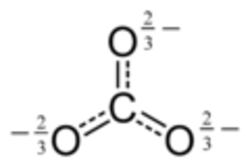
\includegraphics[width=0.2\columnwidth]{Pictures/Carbonate2.pdf} 
\quad \quad
\includegraphics[width=0.13\columnwidth]{Pictures/Carbonate3.pdf} 
\end{center}
\caption{A gauche : une représentation de l'ion carbonate qui respecte la symétrie de la molécule. Les charges négatives sont délocalisées. A droite : une représentation à 3 dimension en termes du volume occupé par chaque atome.
}
\label{fig:Carbonate2}
\end{figure}



L'ion carbonate (voir figure \ref{fig:Carbonate1}) a la formule chimique CO$_3^{2-}$. C'est une molécule plane, avec l'atome de carbone au centre. Naïvement, l'atome de carbone devrait avoir une liaison double (plus courte) vers un atome d'oxygène, et deux liaisons simples (plus longues) vers 2 ions oxygène. Mais ceci brise la symétrie de la molécule, qui a 3 liaisons de même longueur, et 3 atomes d'oxygène équivalents. La symétrie observée expérimentalement (voir figure \ref{fig:Carbonate2}) peut s'expliquer par le phénomène de résonance quantique. \\

Les 3 configurations possibles de l'ion carbonate sont illustrées à la Figure \ref{fig:Carbonate1}. Notons ces configurations $\vert 1 \rangle$, $\vert 2 \rangle$, et $\vert 3 \rangle$. La molécule peut effectuer des transitions entre ces configurations. Nous pouvons donc modéliser l'Hamiltonien du système par
\begin{equation}
H= E_0 \Big (\vert 1\rangle \langle 1\vert + 
\vert 2\rangle \langle 2\vert  +\vert 3\rangle \langle 3\vert  \Big)
-
A \Big( \vert 2\rangle \langle 1\vert + 
\vert 3\rangle \langle 2\vert  +\vert 1\rangle \langle 3\vert + \mathrm{h.c.} \Big)
\label{Eq:CO3}
\end{equation}
où $E_0$ est l'énergie des différentes configurations si on ne tient pas compte des transitions, les termes proportionels à $A$ tiennent compte des transitions possibles entre configurations, et ``h.c.'' veut dire ``hermitien conjugué''.
\begin{enumerate}

\item Quelles sont les énergies des 3 états propres de l'Hamiltonien $H$ défini par l'équation \eqref{Eq:CO3} (en termes des paramètres $E_0$ et $A$) ? \\

\ans{
Dans la base $\lbrace\ket{1},\ket{2},\ket{3}\rbrace$ des états de configuration électronique de l'ion carbonate, l'opérateur hermitien $\hat H$ se représente par la matrice
\begin{equation}
H = \left[
\begin{array}{ccc}
E_0 & -A & -A \\
-A & E_0 & -A \\
-A & -A & E_0
\end{array}
\right].
\end{equation}
L'hermiticité de $\hat H$ implique que les paramètres $E_0$ et $A$ sont des nombres réels. Les valeurs propres $\lambda$ de $H$ vérifient l'équation caractéristique $\det (H - \lambda I) = 0$ qui se simplifie en
\begin{equation}
\begin{split}
&\lambda^3 - 3 E_0 \lambda^2 + (3 E_0^2-3A^2)\lambda + (2A^3+3A^2E_0 - E_0^3) = 0 \\
&\Leftrightarrow (E_0 +A -\lambda)^2 (E_0 -2 A - \lambda) = 0.
\end{split}
\end{equation}
Nous obtenons deux valeurs propres 
\begin{equation}
\boxed{ \lambda_+ = E_0+A \text{ et } \lambda_- = E_0 - 2 A }
\end{equation}
de multiplicités algébriques respectives $\mu_A^+ = 2$ et $\mu_A^- = 1$.\\

\textbf{Note pratique sur l'organisation du calcul :} pour trouver les racines du polynôme caractéristique à la main, un raccourci de notation évident est de poser $\xi \equiv \lambda - E_0$. On obtient alors une équation cubique en $\xi$ qui est $\xi^3 - 3 A^2 \xi + 2 A^3=0$. On remarque immédiatement que les solutions seront de la forme $\xi = \sigma A$ (car alors, les 3 termes de l'équation sont tous cubiques en $A$). Il faut donc trouver $\sigma$ comme solution de $\sigma^3 - 3 \sigma + 2 = 0$. On peut essayer des entiers, et on constate que $\sigma = 1$ et $\sigma = -2$ conviennent. Il suffit ensuite d'écrire l'équation caractéristique sous la forme $(\sigma - 1)(\sigma + 2)(\sigma - \sigma_0) = 0$, et déterminer $\sigma_0$ pour reproduire le polynôme caractéristique. On obtient $\sigma_0 = 1$ en annulant le terme quadratique qui n'existait pas dans ce polynôme. On obtient donc $(\sigma-1)^2 (\sigma + 2) = 0$. \hfill $\square$
}

\item Quels sont les états propres de $\hat  H$ ? \\

\ans{
Comme $H$ est symétrique réelle, elle est nécessairement diagonalisable par transformation orthogonale et donc la multiplicité géométrique $\mu_G$ de toute valeur propre est égale à sa multiplicité algébrique. Ainsi, $\mu_G^+ = \mu_A^+ = 2$ on s'attend donc à trouver 2 vecteurs linéairement indépendants associés à $\lambda_+$. 
\begin{equation}
H - \lambda_+ I = -A \left[
\begin{array}{ccc}
1 & 1 & 1 \\
1 & 1 & 1 \\
1 & 1 & 1 
\end{array}
\right] \Rightarrow 
\ket{\lambda_+} = \alpha \ket{1} + \beta \ket{2} - (\alpha+\beta)\ket{3}.
\end{equation}
On peut se donner, à partir de là, deux vecteurs propres orthogonaux qui formeront la base du sous-espace propre de $\lambda_+$. Nous les noterons $\ket{\lambda_+^{(1)}}$ et $\ket{\lambda_+^{(2)}}$. Considérons, par exemple, la classe de vecteurs avec $\beta = 0$. Ils sont colinéaires au vecteur normé
\begin{equation}
\ket{\lambda_+^{(1)}} \equiv \frac{1}{\sqrt{2}} (\ket{1} - \ket{3}).
\end{equation}
On construit maintenant
\begin{equation}
\ket{\lambda_+^{(2)}} \equiv \alpha' \ket{1} + \beta' \ket{2} - (\alpha'+\beta')\ket{3}.
\end{equation}
et on ajuste $\alpha'$ et $\beta'$ tels que $\braket{\lambda_+^{(1)}|\lambda_+^{(2)}} = 0$ et $\braket{\lambda_+^{(2)}|\lambda_+^{(2)}} = 1$. La première condition donne $2\alpha'+\beta'=0$ ce qui détermine $\beta'$. $\alpha'$ est fixé par la seconde condition qui impose que $2(\alpha'^2 +\alpha'\beta'+\beta'^2) = 6\alpha'^2 = 1$, soit $\alpha' = \frac{1}{\sqrt{6}}$. Le vecteur
\begin{equation}
\ket{\lambda_+^{(2)}} = \frac{1}{\sqrt{6}} ( \ket{1} -2 \ket{2} + \ket{3}).
\end{equation}
convient ainsi pour compléter la base orthonormée du sous-espace $M_+ \equiv \ker \, (\hat H - \lambda_+ \hat I)$. Le dernier vecteur propre est associé à $\lambda_-$ :
\begin{equation}
H - \lambda_- I = -A \left[
\begin{array}{ccc}
-2 & 1 & 1 \\
1 & -2 & 1 \\
1 & 1 & -2 
\end{array}
\right] \Rightarrow 
\ket{\lambda_-} = \frac{1}{\sqrt{3}} (\ket{1} +  \ket{2} +\ket{3}).
\end{equation}
Une base de vecteurs propres est donc
\begin{equation}
\boxed{
\begin{split}
\ket{\lambda_-} &= \frac{1}{\sqrt{3}} (\ket{1} + \ket{2} + \ket{3}), \\
\ket{\lambda_+^{(1)}} &= \frac{1}{\sqrt{2}} (\ket{1} - \ket{3}), \\
\ket{\lambda_+^{(2)}} &= \frac{1}{\sqrt{6}} (\ket{1} - 2 \ket{2} + \ket{3}). \\
\end{split}
}
\end{equation}
Cette base n'est bien évidemment pas unique, et seulement définie à transformations orthogonales près à l'intérieur du sous-espace $M_+$ !
}

\end{enumerate}

\pagebreak

\paragraph{Question 4} \textit{Particule confinée sur un cercle.} \\

\begin{center}
\begin{tikzpicture}[scale=0.75]
\draw (2,2) circle (3cm);
\draw[dashed] (2,2) -- (5,2);
\node at (3.5,1.7) {$R$};
\end{tikzpicture}
\end{center}

Considérons une particule de masse $m$ confinée sur un cercle de rayon $R$ et de circonférence $L=2 \pi R$. (Plus précisément, il y a un potentiel qui confine la particule dans les directions transverses. Ce potentiel est tellement fort qu'aux échelles d'énergie que nous envisageons, le seul degré de liberté est le mouvement le long du cercle). \\

Soit $x\in[-\frac{L}{2},\frac{L}{2}[$ la coordonnée le long du cercle. Le potentiel est nul tout le long du cercle $V(x)=0$. L'équation de Schrödinger stationnaire pour la particule est donc
\begin{equation}
-\frac{\hbar^2}{2m} \frac{d^2}{d x^2} \psi(x) = E \psi(x)\ .\label{eq:FreeSchrodinger}
\end{equation}
L'origine $x=0$ est choisie arbitrairement, puisque ce système possède une symétrie de rotation.
\begin{enumerate}
\item Quelles sont les conditions de raccord en $x=\pm \frac{L}{2}$ qu'il faut imposer à $\psi(x)$ pour respecter la symétrie du problème ? \\

\ans{
Un cercle de circonférence $L>0$ correspond à la droite réelle repliée sur elle-même où les points $x$ et $x+L$ ont été identifiés. La fonction d'onde définie sur ce cercle doit donc respecter cette périodicité, soit $\psi(-\frac{L}{2}) = \psi(\frac{L}{2})$
et $\frac{d}{d x}\psi(-\frac{L}{2}) = \frac{d}{d x} \psi(\frac{L}{2})$
.
} 

\item Trouver les niveaux d'énergie de la particule confinée sur un cercle, ainsi que la dégénérescence des niveaux, et donner les fonctions d'onde propres de l'hamiltonien. \\

\ans{
On résout l'équation \eqref{eq:FreeSchrodinger} pour la fonction $\psi(x)$. L'espace des solutions est un espace vectoriel de dimension 2 de fonctions réelles à valeurs complexes dont une base est donnée par
\begin{equation}
\psi_+ (x) = \alpha_+ e^{ikx}, \quad \psi_- (x) = \alpha_- e^{-ikx}, \quad k \equiv \sqrt{\frac{2mE}{\hbar^2}} \in \mathbb{R}^+ \label{eq:GenSol}
\end{equation}


Pour trouver les valeurs de $k$ compatibles avec les conditions aux bords, nous pouvons procéder de plusieurs manières.

\begin{itemize}[label=$\rhd$]
\item \textbf{Méthode 1 : argument de parité}. \\
L'Hamiltonien (en tenant compte des conditions aux bords) commute avec l'opérateur parité. Nous pouvons donc choisir les états propres pairs et impairs. Ceux ci sont:
\begin{equation}
\psi_{\text{pair}} (x) = A_p \cos {kx}, \quad \psi_{\text{impair}} (x) = A_i \sin{kx}, \quad k \equiv \sqrt{\frac{2mE}{\hbar^2}} \in \mathbb{R}^+. \label{eq:GenSolPair}
\end{equation}
Les solutions doivent être périodiques de période $L$, ce qui fixe
$k L = 2 \pi n$, $n \in \mathbb{N}$. \\

\item \textbf{Méthode 2 : résolution directe des conditions de raccord}. \\
Nous considérons la solution d'énergie $E$ qui est combinaison linéaire des 2 solutions fondamentales données en \eqref{eq:GenSol} :
\begin{equation}
\psi(x) = \alpha_+ e^{ikx} + \alpha_- e^{-ikx}\ .
\end{equation}
Les conditions aux bords donnent:
\begin{eqnarray}
\psi\Big(-\frac{L}{2}\Big)=\psi\Big(\frac{L}{2}\Big) &\Leftrightarrow & 
 \alpha_+ e^{-\frac{ikL}{2}} + \alpha_- e^{+\frac{ikL}{2}} =  \alpha_+ e^{ +\frac{ikL}{2}} + \alpha_- e^{-\frac{ikL}{2}}\nonumber\\
 \psi'\Big(-\frac{L}{2}\Big)= \psi' \Big(\frac{L}{2}\Big) &\Leftrightarrow & 
 ik\left( \alpha_+ e^{-\frac{ikL}{2}} - \alpha_- e^{+\frac{ikL}{2}} \right)= ik\left(  \alpha_+ e^{+\frac{ikL}{2}} - \alpha_- e^{-\frac{ikL}{2}}\right)\nonumber
\end{eqnarray}
Prenant des combinaisons linéaires des ces équations, nous obtenons
\begin{equation}
\left.
\begin{array}{ccc}
 \alpha_+ e^{-\frac{ikL}{2}}  &=&  \alpha_+ e^{+\frac{ikL}{2}} 
 \\
  \alpha_- e^{+\frac{ikL}{2}} &=&  \alpha_- e^{-\frac{ikL}{2}} 
\end{array}
\right\rbrace \Rightarrow e^{ikL} = 1,
\end{equation}
ce qui impose également que
$ k L = 2\pi n$, $n \in \mathbb{N}$.
\end{itemize}

Imposer une condition de raccord conduit donc à la quantification des niveaux d'énergie. On donne à présent les états propres du système :
\begin{equation}
E_n = \frac{\hbar^2 k_n^2}{2m} = \frac{2\pi^2 \hbar^2 n^2}{m L^2}, \quad \psi_\pm^{(n)} (x) = \frac{1}{\sqrt{L}} e^{\pm \frac{2\pi i}{L}n \, x}.
\end{equation}
L'état fondamental $n=0$ n'est pas dégénéré, tandis que les états excités $n>0$ sont doublement dégénérés. Ceci est dû au fait que la particule libre sur le cercle peut s'y mouvoir dans le sens trigonométrique, ou dans le sens horlogique.
}


\end{enumerate}

\chapter{Août 2019}

\paragraph{Question 1} \textit{Théorie.} \\

Soit $\hat A= \hat A^\dagger$ un opérateur hermitien agissant dans un espace de Hilbert de dimension finie.

\begin{enumerate}

\item Les éléments de matrice de $\hat A^\dagger$ (par exemple $\langle \alpha \vert \hat A^\dagger \vert \beta \rangle$) peuvent s'exprimer en terme des éléments de matrice de $\hat A$. Donner cette relation.\\

\ans{
\begin{equation}
\langle \alpha \vert \hat A^\dagger \vert \beta \rangle=
\overline{\langle \beta \vert \hat A^\dagger \vert \alpha \rangle}
\end{equation}}

\item
Montrer que les valeurs propres de $\hat A$ sont réelles. \\

\ans{
Soit $a$ une valeur propre de $\hat A$ et $\ket{a}$ le vecteur propre associé. On a $\hat A\ket{a} = a\ket{a}$ soit $\braket{a|\hat A|a} = a \braket{a|a}$. D'où $\overline{\braket{a|\hat A|a}} = \bar a \braket{a|a}$. Par ailleurs, $\overline{\braket{a|\hat A|a}} = \braket{a|\hat A^\dagger|a} = \braket{a|\hat A|a}$ d'où finalement $(a-\bar{a})\braket{a|a} = 0$. Un vecteur propre ne pouvant jamais se réduire au vecteur nul, et le produit scalaire hilbertien étant non-dégénéré, il vient $a = \bar a$, soit $a\in\mathbb{R}$.
}

\item
Montrer que les vecteurs propres correspondant à deux valeurs propres distinctes sont orthogonaux. \\

\ans{
Soient $a$ et $a'$ deux valeurs propres distinctes ($a\neq a'$) associées aux vecteurs propres $\ket{a}$ et $\ket{a'}$. On peut calculer directement
\begin{equation}
\braket{a|\hat A|a'} = a' \braket{a|a'}, \label{expr1}
\end{equation}
ou utiliser l'hermiticité
\begin{equation}
\braket{a|\hat A|a'} =\braket{a|\hat A^\dagger|a'} = (\hat A \ket{a})^\dagger \ket{a'} = (a\ket{a})^\dagger \ket{a'} = \bar a \braket{a|a'}. \label{expr2}
\end{equation}
En combinant \eqref{expr1} et \eqref{expr2}, il vient sans peine $(a'-a)\braket{a|a'} = 0$. Comme on a supposé que $a\neq a'$, on déduit le résultat escompté $\braket{a|a'} = 0$. 
}

\end{enumerate}

\paragraph{Question 2} \textit{Oscillateur harmonique quantique.} \\

Considérons un oscillateur harmonique de pulsation propre $\omega$. En unités sans dimensions ($\hbar=1$), les opérateurs position $\hat X$ et impulsion $\hat P$ obéissent à la relation de commutation canonique $[\hat X, \hat P]=i $. \\

Les opérateurs de création et destruction sont définis par 
$\hat a= \frac{1}{\sqrt{2}}(\hat X+i\hat P)$, $a^\dagger= \frac{1}{\sqrt{2}}(\hat X-i\hat P)$ et satisfont donc $[\hat a,\hat a^\dagger]=1$. \\

L'opérateur nombre $\hat N$ est donné par $\hat N= \hat a^\dagger \hat a$ et ses vecteurs propres sont notés $\hat N \ket{n} =n \ket{n}$ où $n \in \mathbb{N}$. On peut montrer que $\hat a \ket{n} =\sqrt{n} \ket{n-1}$ et que $\hat a^\dagger \ket{n} =\sqrt{n+1} \ket{n+1}$. L'hamiltonien de l'oscillateur harmonique est $\hat H = \frac{1}{2}\omega ( \hat P^2 + \hat X^2 )\ $. \\

Soit l'état quantique 
\begin{equation}
\vert \psi \rangle = 
 \frac{1}{\sqrt{5}}\vert 0\rangle -  \frac{1}{\sqrt{5}}\vert 1\rangle  - \frac{1}{\sqrt{5}}\vert 2\rangle + \frac{\sqrt{2}}{\sqrt{5}}\vert 4\rangle \ .
 \label{Eq:psi}
\end{equation}

Considérons l'opérateur
\begin{equation}
\hat \Pi_{\text{pair}}=\sum_{m=0}^\infty \vert 2m \rangle \langle 2m \vert \ .
\end{equation}


\begin{enumerate}
\item Que vaut $\langle \psi \vert a \vert \psi \rangle$ ? \\

\ans{
On calcule aisément que 
$ a \vert \psi \rangle = 
-  \frac{1}{\sqrt{5}}\vert 0\rangle  - \frac{\sqrt{2}}{\sqrt{5}}\vert 1\rangle + \frac{2\sqrt{2}}{\sqrt{5}}\vert 3\rangle$.

Par conséquent
$\langle \psi \vert a \vert \psi \rangle = -  \frac{1}{{5}} -  \frac{\sqrt{2}}{{5}} = -  \frac{1+ \sqrt{2}}{{5}}$
}


\item L'opérateur $\hat \Pi_{\text{pair}}$ est hermitien. Montrer que c'est un projecteur. \\

\ans{
Pour montrer que $\hat \Pi_{\text{pair}}$ est un projecteur, il faut prouver que l'opérateur est idempotent $\hat \Pi_{\text{pair}}^2 = \hat \Pi_{\text{pair}}$. Il suffit d'utiliser l'orthogonalité des vecteurs de la base de Fock $\lbrace \ket{n}\rbrace_{n\in\mathbb{N}}$.
\begin{equation}
\hat \Pi_{\text{pair}}^2 = \sum_{m,n=0}^\infty \ket{2m}\braket{2m|2n}\bra{2n} = \sum_{m,n=0}^\infty \ket{2m} \bra{2n} \delta_{m,n} = \sum_{m=0}^\infty \ket{2m}\bra{2m} = \hat \Pi_{\text{pair}}.
\end{equation}
Vu que $\hat \Pi_{\text{pair}}$ est également hermitien, il s'agit d'un projecteur orthogonal. 
}


\item Puisque $\hat \Pi_{\text{pair}}$ est un projecteur, la mesure de cet opérateur ne peut donner que deux résultats : $0$ ou $1$. Si on mesure l'opérateur $\hat \Pi_{\text{pair}}$ sur l'état $\vert \psi \rangle$, quelle est la probabilité de trouver le résultat $1$ ? \\

\ans{
On remarque que $\hat \Pi_{\text{pair}}$ est diagonal dans la base des états propres d'énergie. Ses vecteurs propres sont ainsi les vecteurs propres d'énergie. En tant que projecteur, il possède 2 valeurs propres $1$ et $0$. Chacune de ces valeurs propres sont infiniment dégénérées, car n'importe quel vecteur $\ket{2n}$ pour tout $n\in\mathbb{N}$ est vecteur propre de $\hat \Pi_{\text{pair}}$ avec valeur propre $1$
\begin{equation}
\hat \Pi_{\text{pair}} \ket{2n} = \sum_{m=0}^\infty \ket{2m}\braket{2m|2n} = \sum_{m=0}^\infty \ket{2m} \delta_{m,n} = \ket{2n},
\end{equation}
tandis que n'importe quel vecteur $\ket{2n+1}$ est également vecteur propre avec valeur propre $0$
\begin{equation}
\hat \Pi_{\text{pair}} \ket{2n+1} = \sum_{m=0}^\infty \ket{2m}\braket{2m|2n+1} = \sum_{m=0}^\infty \ket{2m} \delta_{2m,2n+1} = 0.
\end{equation}
Mieux encore, l'opérateur $\hat \Pi_{\text{pair}}$ commute donc avec $\hat H$. Les états propres du système sont ainsi organisés selon leur parité. En particulier, $\hat \Pi_{\text{pair}}$ projette sur l'ensemble des états de parité paire de l'oscillateur. Ceci est attendu du fait que le potentiel lui-même possède une parité définie (paire). La densité de probabilité de présence $|\psi(x)|^2$ hérite de cette parité, d'où les fonctions d'onde $\psi(x)$ s'organisent en fonctions paires et impaires. \\

Si le système est dans l'état $\ket{\psi}$, la probabilité de mesurer la parité et d'obtenir $1$ est
\begin{equation}
P(1) = \sum_{n=0}^\infty |\braket{2n|\psi}|^2
\end{equation}
où l'on somme bien évidemment sur la dégénérescence de la valeur propre $1$. On développe
\begin{equation}
P(1) = |\braket{0|\psi}|^2 + |\braket{2|\psi}|^2 + |\braket{4|\psi}|^2 = \frac{1}{5}+\frac{1}{5}+\frac{2}{5} = \boxed{ \frac{4}{5}}
\end{equation}
On vérifie aisément que $P(0) = |\braket{1|\psi}|^2 = 1 - P(1)$.
}
 
\item Si la mesure de $\hat \Pi_{\text{pair}}$ sur l'état $\vert \psi \rangle$ donne le résultat $1$, quel est l'état (normalisé) de l'oscillateur après la mesure ? 

\ans{
Le projecteur va annihiler les composantes des vecteurs qui sont externes au sous-espace propre dans lequel il projette. Ici, le sous-espace en question est l'ensemble des vecteurs engendrés par les vecteurs de base indicés par un nombre pair. L'état (normalisé) après projection est donc
\begin{equation}
\boxed{ \ket{\psi'} = \frac{1}{\sqrt{4}} \left( \ket{0} - \ket{2} + \sqrt{2}\ket{4} \right). }
\end{equation}
}


\end{enumerate}


\paragraph{Question 3} \textit{Systèmes en dimension 2.} \\

Soit un système à spin $1/2$. Une base de l'espace de Hilbert associé est $\lbrace\ket{\uparrow}, \ket{\downarrow}\rbrace$, qui sont les états propres de $\sigma_z$ de valeurs propres $+1$ et $-1$, respectivement. \\

Supposons qu'à l'instant $t=0$, le spin est dans l'état propre de $\sigma_z$ de valeur propre $+1$ : $\ket{\psi(t=0)} = \ket{\uparrow} \ .$ Supposons en outre que le spin est plongé dans un champ magnétique orienté suivant l'axe $x$. Dû à son moment magnétique, l'hamiltonien du spin est donc $H=\omega \, \sigma_x\ .$

\textit{Note :} vous pouvez travailler en unités où $\hbar =1$. \\

\begin{enumerate}
\item
Quel est l'état $\vert \psi(t)\rangle$ à l'instant $t>0$ ? \\



\ans{
Pour un système conservatif, la solution générale de l'équation de Schrödinger $i\frac{d}{dt}\ket{\psi(t)} = \hat H\ket{\psi(t)}$ est donnée par $\ket{\psi(t)} = \hat U(t,t_0) \ket{\psi(t_0)}$ où $\hat U(t,t_0)$ est l'opérateur (unitaire) d'évolution défini par $\hat U(t,t_0) \equiv e^{-i\hat H (t-t_0)}$. Pour pouvoir calculer facilement l'exponentielle de l'opérateur hamiltonien, on effectue un changement de base vers la base d'états propres de $\hat H$. \\

Dans la base des états propres de $\sigma_z$, on a 
\begin{equation}
H = \omega\,\sigma_x = \omega\left[
\begin{array}{cc}
0 & 1 \\
1 & 0
\end{array}
\right].
\end{equation}
Les valeurs propres d'énergie sont donc $\pm \omega$, respectivement associées aux vecteurs propres
\begin{equation}
\begin{split}
\ket{+} = \frac{1}{\sqrt{2}} (\ket{\uparrow}+\ket{\downarrow}), \\
\ket{-} = \frac{1}{\sqrt{2}} (\ket{\uparrow}-\ket{\downarrow}). \label{eq:PlusMoins}
\end{split}
\end{equation}
On peut renverser ces égalités pour obtenir $\ket{\uparrow} = \frac{1}{\sqrt{2}}(\ket{+}+\ket{-})$ et $\ket{\downarrow} = \frac{1}{\sqrt{2}}(\ket{+}-\ket{-})$. On obtient aisément l'expression de l'opérateur d'évolution (on fixe désormais $t_0 = 0$) :
\begin{equation}
\hat U(t) = e^{-i\omega t} \ket{+}\bra{+} + e^{i\omega t} \ket{-}\bra{-}.
\end{equation}
Son action sur l'état initial $\ket{\psi(0)} = \ket{\uparrow}$ est donc
\begin{equation}
\begin{split}
\ket{\psi(t)} &= \hat U(t) \ket{\psi(0)} = \hat U(t) \ket{\uparrow} \\
&= \frac{1}{\sqrt{2}} (e^{-i\omega t} \ket{+}\bra{+} + e^{i\omega t} \ket{-}\bra{-}) (\ket{+}+\ket{-}) \\
&= \frac{1}{\sqrt{2}} (e^{-i\omega t} \ket{+} + e^{i\omega t} \ket{-}).
\end{split}
\end{equation}
On peut réintroduire les définitions \eqref{eq:PlusMoins} pour obtenir le vecteur évolué dans la base originale :
\begin{equation}
\begin{split}
\ket{\psi(t)} &= \frac{1}{2} \Big[  e^{-i\omega t} (\ket{\uparrow}+\ket{\downarrow}) + e^{i\omega t} (\ket{\uparrow}-\ket{\downarrow})  \Big] \\
&= \boxed { \cos \omega t \ket{\uparrow} - i \sin \omega t \ket{\downarrow}. }
\end{split}
\end{equation}
}

\item
En utilisant votre réponse à la question précédente, quelle est la probabilité $P_\uparrow(t)$ qu'une mesure de l'opérateur $\sigma_z$ à l'instant $t$ sur  l'état $\vert \psi(t)\rangle$ donne le résultat $+1$?
\\ 



\ans{
Par le Postulat 3, la probabilité de mesurer $\sigma_z = 1$ à l'instant $t$ équivaut à $P_\uparrow (t) = |\braket{\uparrow|\psi(t)}|^2$. On a donc $P_\uparrow(t) = \cos^2\omega t$.}

\item Faire un graphique de $P_\uparrow(t)$ en fonction du temps.
\\

\item À quels instants $\sigma_z=+1$ avec certitude (c'est-à-dire avec probabilité $1$) ? \\

\ans{
$P_\uparrow(t) = \cos^2\omega t$  vaut $1$ pour les instants discrets $t = \frac{k\pi}{\omega}$ où $k\in\mathbb{N}$.
}


\end{enumerate}

\paragraph{Question 4} \textit{Particule dans un puits de potentiel infini avec une barrière $\delta$.} \\

\begin{figure}[h!]
\centering
\begin{tikzpicture}[scale=0.75]
\draw[->] (-6,0) -- (6,0) node[right]{$x$};
\draw[->] (-6,0) -- (-6,5) node[above]{$V$};
\draw[very thick]  (-4,6) -- (-4,0);
\draw  (-0.1, 4) -- (-0.1,0);
\draw  (-0.1, 4) -- (0.1,4);
\draw  (0.1, 4) -- (0.1,0);
\draw[very thick]  (4,6) -- (4,0);
%\node at (6,-0.5) {$x$};
%\node at (-6.5,5) {$V$};
\node at (-4,-0.5) {$-\frac{L}{2}$};
\node at (0,-0.5) {$0$};
\node at (4,-0.5) {$+\frac{L}{2}$};
\node[above] at (0,4) {$\uparrow$};
\node[above] at (0,4.6) {$\infty$};
\fill[pattern=north east lines, pattern color=black] (4,0) rectangle (4.25,6);
\fill[pattern=north west lines, pattern color=black] (-4,0) rectangle (-4.25,6);
\end{tikzpicture}
\caption{Représentation schématique du potentiel $V(x)$ de l'équation \eqref{Eq:SchrDelta}: $V$ est infini pour $x<-\frac{L}{2}$ et pour $x>\frac{L}{2}$. En outre un potentiel $\delta$ est présent en $x=0$.}
\end{figure}

Considérons une particule de masse $m$ confinée entre $x= -\frac{L}{2}$ et $x =+\frac{L}{2}$. En $x=0$ se trouve une mince barrière de potentiel. Nous modélisons la barrière de potentiel par une fonction $\delta$. \\

L'équation de Schrödinger stationnaire pour la particule est donc
\begin{equation}
-\frac{\hbar^2}{2m} \frac{d^2}{d x^2} \psi(x) + \alpha \delta(x) \psi(x)= E \psi(x)
\label{Eq:SchrDelta}
\end{equation}
avec $\alpha>0$ et les conditions aux bords $\psi(-\frac{L}{2})=\psi(+\frac{L}{2})=0$.


\begin{enumerate}
\item Quels sont les états propres normalisés de l'Hamiltonien lorsque $\alpha=0$ et quelles sont leurs énergies? 
Donner séparément les états propres pairs et impairs.
\\

\ans{
On résout l'équation $-\frac{\hbar^2}{2m} \frac{d^2}{d x^2} \psi(x) = E \psi(x)$ pour la fonction $\psi(x)$. La solution générale est 
\begin{equation}
\psi(x) = A \cos kx + B \sin kx,\, k = \sqrt{\frac{2mE}{\hbar^2}}\in\mathbb{R}.
\end{equation}
Le potentiel étant pair (invariant sous la réflexion $x\to -x$), la probabilité de présence $|\psi(x)|^2$ est paire, et les fonctions d'onde propres possèdent une parité définie.
\begin{itemize}[label=$\rhd$]
\item \underline{\textit{États pairs}} : vu que $\cos(-\theta) = \cos \theta$, ils seront de la forme $\psi^{(p)} (x) = A \cos kx$. On peut toujours fixer la phase telle que $A$ soit un nombre réel. Vu que la fonction d'onde doit s'annuler en $x = \frac{L}{2}$ (la probabilité de présence y est nulle), on obtient une condition de quantification du nombre d'onde :
\begin{equation}
\cos \frac{kL}{2} = 0 \Rightarrow k L = (2n+1)\pi, \, n\in\mathbb{N}.
\label{Eq:cos}
\end{equation}
Noter que $\cos kx$ étant une fonction paire, nous pouvons restreindre aux $k\geq 0$ (les $k$ négatifs donnant la même solution). Ceci implique la restriction aux $n$ entiers positifs dans l'équation \eqref{Eq:cos}.

Les états propres pairs sont donc donnés par
\begin{equation}
\boxed{
\psi_n^{(p)} (x) = A \cos \Big[ \frac{(2n+1)\pi}{L} x \Big], \quad E_n^{(p)} = \frac{(2n+1)^2\pi^2\hbar^2}{2m}, \quad  n\in\mathbb{N}\ .
}
\end{equation}
On détermine enfin la constante de normalisation $A$ :
\begin{equation}
\begin{split}
\int_{-\frac{L}{2}}^{+\frac{L}{2}} dx \, |\psi_n^{(p)} (x)|^2 &= 2 \int_{0}^{\frac{L}{2}} dx \, A^2 \cos^2 \Big[ \frac{(2n+1)\pi}{L} x \Big] \\
&= \int_{0}^{\frac{L}{2}} dx \, A^2 \Big[ 1 + \cos \Big[ (2n+1)\frac{2\pi}{L} x \Big] \Big] \\
&= \frac{L}{2} A^2 + A^2 \Big( (2n+1)\frac{2\pi}{L} \Big)^{-1} \left[ \sin \Big[ (2n+1)\frac{2\pi}{L} x \Big] \right]_{0}^{\frac{L}{2}} \\
&= \frac{L}{2} A^2 \alpha^2 + 0 = 1 \Rightarrow \boxed{A = \sqrt{\frac{2}{L}}.}
\end{split}
\end{equation}
\item \underline{\textit{États impairs}} : vu que $\sin(-\theta) = -\sin \theta$, il s'agit de la branche complémentaire $\psi^{(i)} (x) = B \sin kx$. On fixe à nouveau la phase telle que $B$ soit un nombre réel. L'annulation de la fonction d'onde en $x = \frac{L}{2}$ conduit cette fois à une autre condition de quantification :
\begin{equation}
\sin \frac{kL}{2} = 0 \Rightarrow k L = 2n\pi, \, n\in\mathbb{N}_0.
\label{Eq:sin}
\end{equation}
La fonction $\sin$ étant impaire, nous pouvons restreindre aux $k\geq 0$ (les $k$ négatifs donnant la même solution). En outre $k=0$ donne une solution identiquement nulle, et ne peut donc pas représenter une densité de probabilité de présence (dont l'intégrale du module carré doit donner 1). Pour ces raisons on se restreint aux entiers $n$ strictement positifs dans l'équation \eqref{Eq:sin}.

 Les états propres impairs s'écrivent explicitement :
\begin{equation}
\boxed{
\psi_n^{(i)} (x) = B \sin \Big[ \frac{2n\pi}{L} x \Big], \quad E_n^{(i)} = \frac{(2n)^2\pi^2\hbar^2}{2m}, \quad  n\in\mathbb{N}_0\ .
}
\end{equation}
Il n'est pas difficile de constater que la valeur de la constante de normalisation $B$ est également $B = \sqrt{\frac{2}{L}}$. 
\end{itemize}

Pour conclure, on peut réunir les deux classes de solutions. Les niveaux d'énergie du système sont donnés par
\begin{equation}
\boxed{ E_n = \frac{n^2\pi^2\hbar^2}{2m} }
\end{equation}
où $n$ est un nombre naturel \textit{non-nul}. L'état $n=1$ de plus basse énergie est appelé \textit{niveau fondamental} et possède une énergie résiduelle non-nulle (énergie de point zéro). Les fonctions d'onde associées à ces niveaux d'énergie sont notées $\psi_m (x)$ et possèdent la parité de $m$ :
\begin{equation}
\boxed{
\begin{split}
&\text{ Si } m \text{ est pair, } \psi_m (x) = \sqrt{\frac{2}{L}} \cos \Big( \frac{m\pi}{L}x \Big), \\
&\text{ Si } m \text{ est impair, } \psi_m (x) = \sqrt{\frac{2}{L}} \sin \Big( \frac{m\pi}{L}x \Big).
\end{split} }
\label{Eq:SolutionsGen}
\end{equation}
}

\item Dorénavant nous considérons $\alpha \neq  0$. Quelles sont les conditions de raccord qu'il faut imposer en $x=0$ pour tenir compte du potentiel $\delta$ ? \\

\ans{
Considérons un intervalle centré en $0$ et de rayon $\varepsilon >0$ quelconque fixé, et pouvant être arbitrairement proche de zéro. Intégrons l'équation \eqref{Eq:SchrDelta} sur cet intervalle.
\begin{equation}
-\frac{\hbar^2}{2m} \int_{-\varepsilon}^{+\varepsilon} dx \, \frac{d^2}{d x ^2} \psi(x) + \alpha \int_{-\varepsilon}^{+\varepsilon} dx \, \delta(x) \psi(x) = E \int_{-\varepsilon}^{+\varepsilon} dx \, \psi(x)
\end{equation}
\begin{itemize}[label=$\rhd$]
\item Le premier terme donne $-\frac{\hbar^2}{2m} [\frac{d\psi}{dx}(+\varepsilon) - \frac{d\psi}{dx}(-\varepsilon)]$ en vertu du Théorème Fondamental du Calcul Intégral.
\item Pour évaluer le second terme, on sait que la distribution $\delta(x)$ peut se représenter comme une fonction impropre nulle presque partout sur $\mathbb{R}$, sauf en $x = 0$ où elle prend une valeur techniquement infinie pour assurer que $\int_{\mathbb{R}} dx \, \delta (x) = 1$. Modifier le rayon $\varepsilon$ de l'intervalle d'intégration ne change donc pas la valeur numérique du second terme, qui peut donc se ramener à $\alpha \int_{\mathbb{R}} dx \, \delta(x)\psi(x) = \alpha \psi(0)$.
\item Le dernier terme peut être majoré grâce à la monotonie de l'intégrale. En effet, vu que la densité de probabilité de présence ne peut jamais être infinie en un point, on a $|\psi(x)| \leq \kappa$, $\forall x \in [-\varepsilon,+\varepsilon]$, où $\kappa$ est un réel positif. Donc
\begin{equation}
E \left|\int_{-\varepsilon}^{+\varepsilon} dx \, \psi(x)\right| \leq E \int_{-\varepsilon}^{+\varepsilon} dx \, |\psi(x)| \leq 2\varepsilon E \kappa = \mathcal{O}(\varepsilon).
\end{equation}

\end{itemize}
En prenant la limite $\varepsilon\to 0$, il vient donc $-\frac{\hbar^2}{2m} [\frac{d\psi}{dx}(0^+) - \frac{d\psi}{dx}(0^-)] + \alpha \psi(0)=0$ soit
\begin{equation}
\frac{d\psi}{dx}(0^+) - \frac{d\psi}{dx}(0^-) = \frac{2m\alpha}{\hbar^2} \psi(0). \label{eq:RaccordDerivee}
\end{equation}
En intégrant une seconde fois sur $[-\varepsilon,+\varepsilon]$, on montre de manière analogue que la fonction d'onde doit être continue en $0$, soit $\psi(0^-) = \psi(0^+)$. 
}

\item
Le potentiel dans l'équation \eqref{Eq:SchrDelta} est pair. Par conséquent les fonctions d'ondes propres commutent avec l'opérateur parité, et peuvent donc être choisies paires ou impaires.

Montrer que les fonctions d'ondes impaires solutions de l'équation avec $\alpha=0$ (trouvées au point 1) sont aussi solutions quand $\alpha\neq 0$ avec la même énergie. \\

\ans{
Considérons $\psi_m(x)$ solutions de l'équation de Schrödinger sans potentiel dérivées obtenues à l'équation \eqref{Eq:SolutionsGen}, et réduisons-nous à $m = 2n+1$ impair. Sur $[-\frac{L}{2},+\frac{L}{2}]\setminus \lbrace 0 \rbrace$, l'équation \eqref{Eq:SchrDelta} se réduit à $-\frac{\hbar^2}{2m} \frac{d^2}{d x^2} \psi(x) = E \psi(x)$ dont les $\psi_m(x)$ sont solutions par définition. Il reste donc à vérifier qu'elles satisfont les nouvelles conditions de raccord rendues nécessaires par la présence du potentiel $\delta$ inséré en $x=0$. \\

Les $\psi_m(x)$ sont continûment différentiable en $x=0$. On a vu au point précédent que lorsque $\alpha\neq 0$, la dérivée première de la fonction d'onde subit un saut dont l'amplitude dépend linéairement de $\psi(0)$. Vu que $\psi_m (0) = 0$ du fait de leur parité impaire, la dérivée doit être continue, aussi bien que la fonction d'onde elle-même. Ce qui est bien le cas !
}
 

\item Considérons maintenant les solutions paires. En utilisant la condition de raccord trouvée au point 2, déterminer les niveaux d'énergie de ces solutions. 

\textit{Note :} Ces niveaux d'énergie seront donnés par une équation transcendante que vous ne pourrez pas résoudre explicitement ! \\

\ans{
On démarre à nouveau en résolvant l'équation de Schrödinger dans la zone $0 < x <\frac{L}{2}$. Il vient comme au point 1 $\psi_+ (x) = A \cos k x  + B \sin k x$ où $\hbar k = \sqrt{2mE}$. La fonction étant paire, on peut directement déterminer sa forme dans la zone $-\frac{L}{2}<x<0$, c'est-à-dire $\psi_- (x) = A \cos kx - B \sin kx$. La fonction doit s'annuler aux bords $x=\pm\frac{L}{2}$. Il est bien évidemment suffisant de le vérifier pour, disons, $x = \frac{L}{2}$, ce qui donne :
\begin{equation}
A \cos \frac{kL}{2} + B \sin \frac{kL}{2} = 0 \Rightarrow B = -A \cot \frac{kL}{2}.
\end{equation}

Appliquons maintenant les conditions de raccord en $x=0$. 

La fonction d'onde est 
 continue et vaut $\psi_+ (0) = \psi_- (0) = A$. 
 
On calcule le saut de dérivée première
\begin{equation}
\psi'_+ (0) - \psi'_- (0) = \frac{2m\alpha}{\hbar^2} \psi(0) \Leftrightarrow 2kB = \frac{2m\alpha}{\hbar^2} A \ .
\end{equation}
En introduisant la relation qui donne $B$ en terme de $A$, il vient
\begin{equation}
\cot \frac{kL}{2} =- \frac{m\alpha}{\hbar^2 k} \quad \Rightarrow\quad \boxed{ \cot\zeta = - \frac{m L\alpha} {2 \hbar^2}\frac{1}{\zeta},\ \zeta\equiv \frac{kL}{2}. }
\end{equation}
Quand $\alpha=0$ on retrouve le solutions trouvées précédemment: $\zeta_n = (2n+1) \pi/2$, $n\in\mathbb{N}_0$. On voit aussi facilement que quand $\alpha>0$, $\zeta_n$ est plus grand que quand $\alpha=0$, c'est à dire que la présence du potentiel $\alpha \delta(x)$ augmente l'énergie des états propres, ce à quoi on pouvait s'attendre. Mais pour avoir une solution précise, il faudrait résoudre cette équation transcendante numériquement ! 
}
\end{enumerate}

\chapter{Juin 2021}

\paragraph{Question 1} \textit{Oscillateur harmonique quantique.} \\

Considérons un oscillateur harmonique de pulsation propre $\omega$. En unités sans dimensions ($\hbar=1$), les opérateurs position $\hat X$ et impulsion $\hat P$ obéissent à la relation de commutation canonique $[\hat X, \hat P]=i $. \\

Les opérateurs de création et destruction sont définis par 
$\hat a= \frac{1}{\sqrt{2}}(\hat X+i\hat P)$, $a^\dagger= \frac{1}{\sqrt{2}}(\hat X-i\hat P)$ et satisfont donc $[\hat a,\hat a^\dagger]=1$. \\

L'opérateur nombre $\hat N$ est donné par $\hat N= \hat a^\dagger \hat a$ et ses vecteurs propres sont notés $\hat N \ket{n} =n \ket{n}$ où $n \in \mathbb{N}$. On peut montrer que $\hat a \ket{n} =\sqrt{n} \ket{n-1}$ et que $\hat a^\dagger \ket{n} =\sqrt{n+1} \ket{n+1}$. L'hamiltonien de l'oscillateur harmonique est $\hat H = \frac{1}{2}\omega ( \hat P^2 + \hat X^2 )\ $. \\

Soit l'état quantique 
\begin{equation}
\vert \psi \rangle = 
 \frac{1}{\sqrt{2}}\ket{0}  - \frac{1}{\sqrt{2}}\ket{2} \ .
 \label{Eq:psi}
\end{equation}

\begin{enumerate}


\item 
Supposons qu'à l'instant $t=0$, l'oscillateur harmonique est dans l'état $\ket{\psi}$ donné par l'équation \eqref{Eq:psi}. Quel est son état $\ket{\psi(t)}$ à l'instant $t>0$ ?

\item 
Que vallent 
\begin{eqnarray}
&\langle P(t) \rangle = \braket{\psi (t)|\hat P|\psi(t)}&\\
&\langle X(t) \rangle = \braket{\psi(t)|\hat X|\psi(t)}&\\
&\braket{\psi(t)|\left( \hat P^2 + \hat X^2\right)|\psi(t)}\quad  ?&
\end{eqnarray}

\item 
Calculer les incertitudes de la position $\Delta X^2(t)$ et 
et de l'impulsion $\Delta P^2(t)$ dans l'état $\ket{\psi(t)}$.


\item Faire un graphique dans lequel vous représenterez  $\Delta X^2(t)$ et $\Delta P^2(t)$ en fonction du temps. N'oubliez pas d'annoter les axes du graphique.

\end{enumerate}

Prévoir une page quadrillée pour le graphique.

\paragraph{Question 2} \textit{Système de dimension 2.} \\

\begin{figure}[h!]
\begin{center}
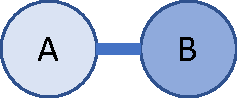
\includegraphics[width=0.3\columnwidth]{Pictures/AB.pdf} 
\end{center}
\caption{Molécule composée de deux atomes A et B.
}
\label{fig:AB}
\end{figure}

Nous considérons une molécule composée de deux atomes A et B. Nous considérons un électron dont le dynamique peut-être analysée indépendemment des autres électrons qui composent la molécule.

Nous notons $\ket{A}$ l'état de l'électron si il se trouve autour de l'atome A. Dans ce cas son énergie est $+ 4 E_0$.

Nous notons $\ket{B}$ l'état de l'électron si il se trouve autour de l'atome B. Dans ce cas son énergie est $- 4 E_0$.

L'électron a aussi une amplitude de passer de l'atome A à l'atome B.

L'espace de Hilbert de l'électron peut être approximé par un espace à 2 états dont une base orthonormée est $\{\ket{A}, \ket{B}\}$. Dans cette base l'Hamiltonien prends la forme
\begin{equation}
H = E_0 \begin{pmatrix}
+4 & +3 \\
+3 & -4 & 
\end{pmatrix}
\end{equation}

\begin{enumerate}
\item Donner les valeurs propres et les vecteurs propres de H.

\item Supposons qu'à l'instant $t=0$ l'électron se trouve dans l'état $\ket{\psi(t=0)}=\ket{A}$. Quel est sont état $\ket{\psi(t)}$ en $t>0$? Exprimer cet état dans la base $\{\ket{A}, \ket{B}\}$.

\item Pour l'état $\ket{\psi(t)}$, la probabilité $P(B)$ de trouver l'électron dans l'état $\ket{B}$ change au cours du temps. A quels instants  $P(B)$ est il maximal? Quelle est la valeur maximale de $P(B)$?

\end{enumerate}

\paragraph{Question 3} \textit{Particule dans un champ de graviation.} \\

\begin{figure}[h!]
\begin{center}
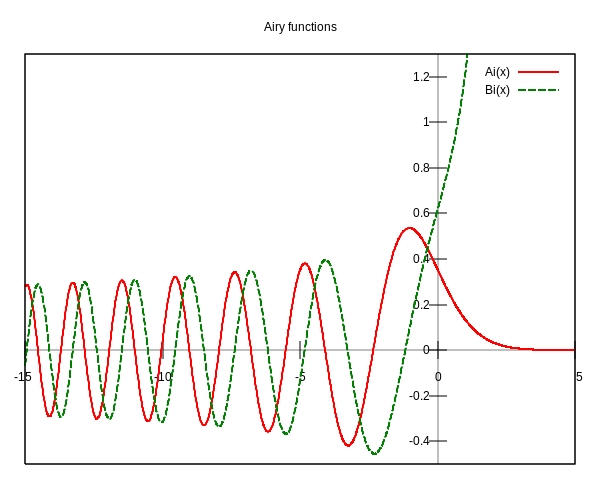
\includegraphics[scale=0.6]{Pictures/Airy_plot.svg.png} 
\end{center}
\caption{Graphique des deux solutions linéairement indépendantes de l'équation d'Airy, notées $Ai(x)$ et $Bi(x)$.
}
\label{fig:Airy}
\end{figure}

Soit un particule de masse $m$ soumis à la pesanteur, et limité à la région des $z$ positifs. 
Le potentiel que voit la particule est donc
\begin{eqnarray}
V(z)&=& mgz \quad z>0 \nonumber\\
&=& +\infty \quad z\leq 0 \ .
\end{eqnarray}

La trajectoire classique de cette particule est  une série de chutes libres, séparées par des rebonds lorsque la particule atteint $z=0$ lorsque sa vitesse change de signe).

Classiquement l'énergie minimale de cette particule est $E=0$, correspondant à la particule au repos en $z=0$.

Nous désirons étudier les états stationnaires de ce système $\psi(z)$, solutions de l'équation de Schrödinger
\begin{equation}
\left( -\frac{\hbar^2}{2m}\partial_z^2 + V(z) \right) \psi (z)= E \psi (z)\ .
\label{Eq:Schg}
\end{equation}
et en particulier déterminer l'énergie de l'état fondamental.

\begin{enumerate}

\item
Utilisez le principe d'incertitude pour estimer la hauteur moyenne $\langle z  \rangle$ à laquelle se trouve la particule, et son énergie, lorsqu'elle est dans l'état d'énergie minimum, en fonction de $m$, $g$, $\hbar$. Donner les valeurs de cette hauteur moyenne et de cette énergie dans le cas d'un électron dans le champ de pesanteur terrestre.

\item
Quelle sont les conditions que doit satisfaire $\psi(z)$ en $z=0$ et pour $z\to +\infty$ pour être un état propre de l'Hamiltonien?

\item
Faites un changement de variables 
\begin{equation}
z \to x = \alpha (z-z_0)
\end{equation}
pour ramener l'équation Eq. (\ref{Eq:Schg}) à la forme
\begin{equation}
\partial_{x}^2  \psi (x) - x \psi (x)= 0 .
\label{Eq:SchgB}
\end{equation}

\item 
Quelles sont les conditions que doit obéir $\psi(x) $ pour être un état propre de l'Hamiltonien?

\item
L'équation  Eq. (\ref{Eq:SchgB}) est connue sous le nom d'équation d'Airy. Les deux solutions linéairement indépendantes de l'équation d'Airy sont notées $Ai(x)$ et $Bi(x)$. Leur graphique est donné dans la figure. 

Pour $x$ grand positifs, ces fonctions se comportent comme 
\begin{eqnarray}
Ai(x)  &\simeq& a e^{- \frac{2}{3} x^{3/2}} \quad \text{lorsque } x\gg 0 \quad \text{(décroit exponentiellement)}\\
Bi(x)  &\simeq&  b e^{+ \frac{2}{3} x^{3/2}} \quad \text{lorsque } x\gg 0 \quad \text{(croit exponentiellement)}
\end{eqnarray}
avec $a$ et $b$ des constantes.

Ces deux fonctions oscillent pour $x$ négatifs. Les premiers zéros de $Ai(x)$ sont approximativement $-2.33811$, $-4.08795$, $-5.52056$.
Les premiers zéros de  $Bi(x)$  sont approximativement $-1.17371$,  $ -3.27109$, $-4.83074$.

Utilisez ces résultats pour donner l'énergie $E_0$ de l'état fondamental de $H$ et l'énergie $E_1$ du premier état excité, en fonction de $m$, $g$, $\hbar$.
Comparez avec votre estimation obtenue au point 1.

\end{enumerate}

\chapter{Août 2021}

\paragraph{Question 1} \textit{Oscillateur harmonique quantique.} \\

Considérons un oscillateur harmonique de pulsation propre $\omega$. En unités sans dimensions ($\hbar=1$), les opérateurs position $\hat X$ et impulsion $\hat P$ obéissent à la relation de commutation canonique $[\hat X, \hat P]=i $. \\

Les opérateurs de création et destruction sont définis par 
$\hat a= \frac{1}{\sqrt{2}}(\hat X+i\hat P)$, $a^\dagger= \frac{1}{\sqrt{2}}(\hat X-i\hat P)$ et satisfont donc $[\hat a,\hat a^\dagger]=1$. \\

L'opérateur nombre $\hat N$ est donné par $\hat N= \hat a^\dagger \hat a$ et ses vecteurs propres sont notés $\hat N \ket{n} =n \ket{n}$ où $n \in \mathbb{N}$. On peut montrer que $\hat a \ket{n} =\sqrt{n} \ket{n-1}$ et que $\hat a^\dagger \ket{n} =\sqrt{n+1} \ket{n+1}$. L'hamiltonien de l'oscillateur harmonique est $\hat H = \frac{1}{2}\omega ( \hat P^2 + \hat X^2 )\ $. \\

Les fonctions d'onde des 2 premiers états propres de l'Hamiltonien sont 
$$\psi_0(x)=\langle x \vert 0\rangle = \frac{1}{\pi^{1/4}} e^{-x^2/2}$$
et
$$\psi_1(x)=\langle x \vert 1\rangle = \frac{1}{\pi^{1/4}} \sqrt{2} x e^{-x^2/2}\ .$$
Ces fonctions d'onde sont représentées à la figure \ref{fig:Psi01}.


\begin{figure}[h!]
\begin{center}
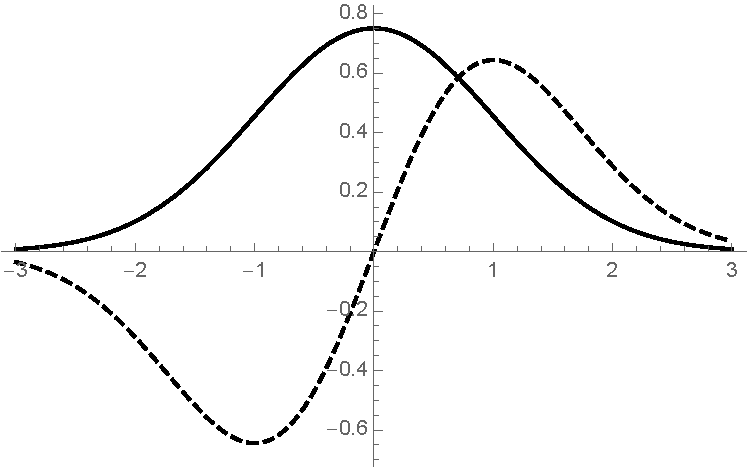
\includegraphics[width=0.5\columnwidth]{Pictures/Psi0Psi1.pdf} 
\end{center}
\caption{Fonctions d'onde des deux premiers états propres de l'oscillateur harmonique $\psi_0(x)=\langle x \vert 0\rangle$ et $\psi_1(x)=\langle x \vert 1\rangle$. }
\label{fig:Psi01}
\end{figure}

Soit l'état quantique 
\begin{equation}
\vert \psi \rangle = 
 \frac{1}{\sqrt{2}}\ket{0}  +  \frac{1}{\sqrt{2}}\ket{1}\ .
 \label{Eq:psi}
\end{equation}

\begin{enumerate}


\item 
Supposons qu'à l'instant $t=0$, l'oscillateur harmonique est dans l'état $\ket{\psi}$ donné par l'équation \eqref{Eq:psi}. Quel est son état $\ket{\psi(t)}$ à l'instant $t>0$ ?

\item 
Que vallent 
\begin{eqnarray}
&\langle P(t) \rangle = \braket{\psi (t)|\hat P|\psi(t)}&\\
&\langle X(t) \rangle = \braket{\psi(t)|\hat X|\psi(t)}&\\
&\braket{\psi(t)| \hat X^2 |\psi(t)}\quad  ?&
\end{eqnarray}




\item Soit les instants suivants 
\begin{equation}
t_k= k \frac{\pi}{4} \frac{1}{\omega}\quad , \quad k=0,1,2,3,4,5,6,7 \ .\label{Eq:tk}
\end{equation}


Les panneaux de la figure \ref{FigPsi2} représentent la densité de probabilité 
\begin{equation}
\vert \psi(x,t)\vert^2 = \vert \langle x \vert \psi(t) \rangle \vert^2
\end{equation}
 à certains instants $t$, avec $t \in \{t_0,...,t_7\}$.

De quels instants $t_k$ s'agit-il?   Justifiez votre réponse. 
(La réponse attendue est de la form "Le panneau (A) représente   $ \vert \psi(x,t)\vert^2$ aux instants $t_2$ et $t_7$ parceque... ."


\begin{figure}
    \centering
    \begin{subfigure}[t]{0.4\textwidth}
        \centering
        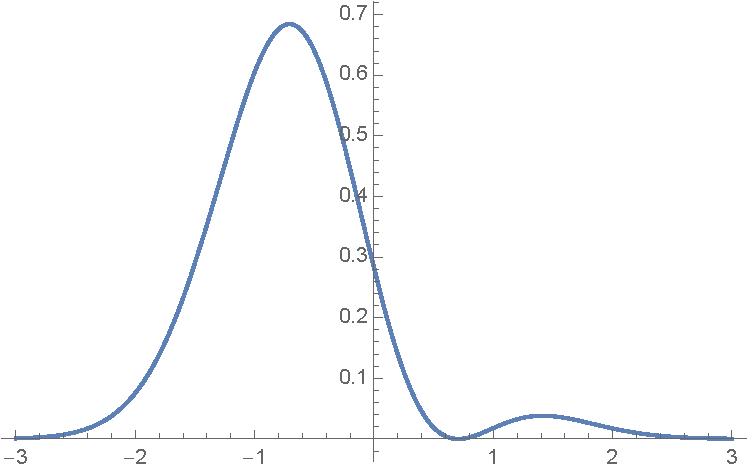
\includegraphics[width=\linewidth]{Pictures/FigPsi4.pdf}
        \caption{} \label{fig:timingA}
    \end{subfigure}
    \hfill
    \begin{subfigure}[t]{0.4\textwidth}
        \centering
        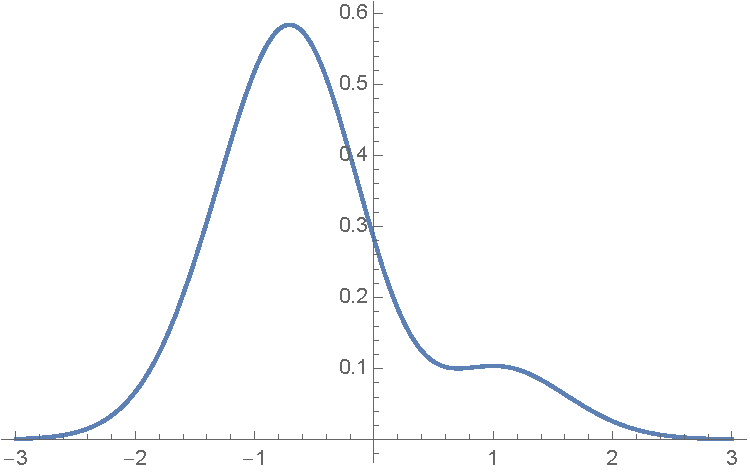
\includegraphics[width=\linewidth]{Pictures/FigPsi3.pdf} 
        \caption{} 
        \label{fig:timingB}
    \end{subfigure}
  

    \vspace{1cm}
   \begin{subfigure}[t]{0.4\textwidth}   
        \centering
        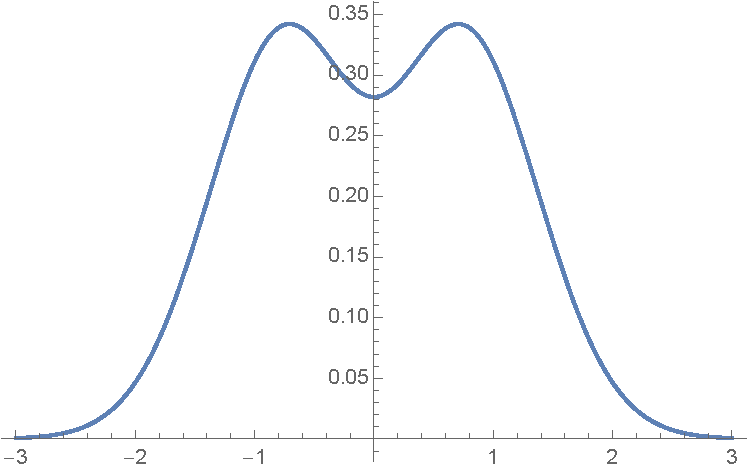
\includegraphics[width=\linewidth]{Pictures/FigPsi2.pdf}
        \caption{} \label{fig:timingC}
    \end{subfigure}
    \hfill
    \begin{subfigure}[t]{0.4\textwidth}
        \centering
        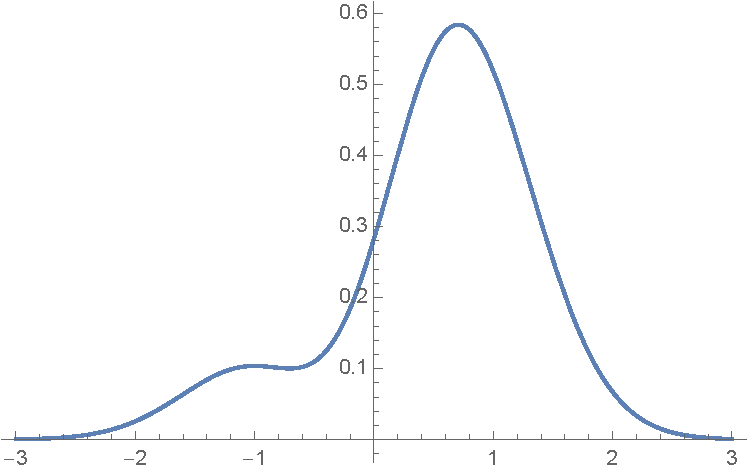
\includegraphics[width=\linewidth]{Pictures/FigPsi1.pdf} 
        \caption{} 
        \label{fig:timingD}
    \end{subfigure}
    
    \vspace{1cm}
   \begin{subfigure}[t]{0.4\textwidth}
    \hfill       
        \centering
        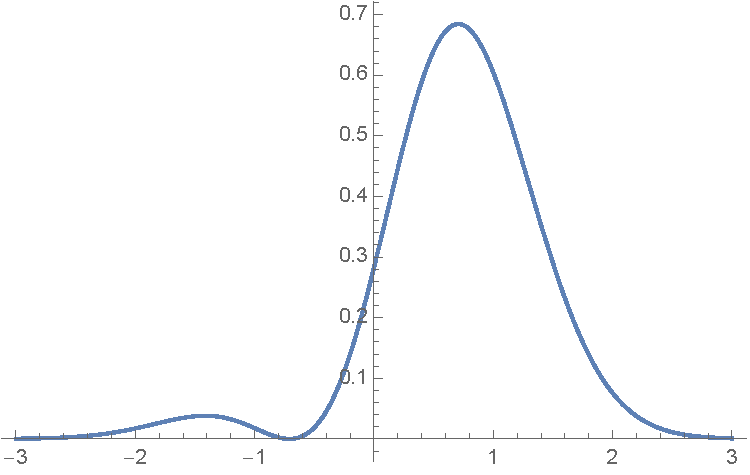
\includegraphics[width=\linewidth]{Pictures/FigPsi0.pdf}
        \caption{} \label{fig:timingE}
    \end{subfigure}
 
        
    \caption{Les panneaux (A) (B) (C) (D) (E) représentent la densité de probabilité 
$ \vert \psi(x,t)\vert^2$ à certains des instants $t_k$ donnés à l'équation \eqref{Eq:tk}.}
\label{FigPsi2}
\end{figure}





\end{enumerate}

\paragraph{Question 2} \textit{Changement de base.} \\

Les opérateurs sans dimension position $\hat x$ et impulsion $\hat p$ satisfont 
\begin{equation}
[\hat x, \hat p ] = i\ .
\label{xp:1}
\end{equation}
Les états propres de l'opérateur position sont notés $\vert x \rangle$ et satisfont
\begin{eqnarray}
\hat x \vert x \rangle &=& x\vert x \rangle \ ,\label{xp:2B}\\
\langle x' \vert x \rangle &=& \delta (x-x') \ .
\label{xp:2}
\end{eqnarray}
Pour tout état $\vert \psi \rangle$ nous avons
\begin{eqnarray}
\langle x \vert \hat x \vert \psi \rangle &=& x  \langle x  \vert \psi \rangle \ ,
\label{xp:3}\\
\langle x \vert \hat p \vert \psi \rangle &=& -i \partial_x  \langle x  \vert \psi\rangle\ . \label{xp:4}
\end{eqnarray}

Considérons les opérateurs obtenus par une rotation d'angle $\theta$ de l'espace des phases
\begin{eqnarray}
\hat u  &=&  \cos \theta\  \hat x + \sin \theta\   \hat p\ ,
\label{xp:5}\\
\hat v  &=&  - \sin \theta \  \hat x + \cos \theta \  \hat p \label{xp:6}\ .
\end{eqnarray}
Nous avons aussi la transformation inverse
\begin{eqnarray}
\hat x  &=&  \cos \theta\   \hat u - \sin \theta\   \hat v\ ,
\label{xp:7}\\
\hat p  &=&   \sin \theta\   \hat u + \cos \theta\   \hat v \label{xp:8}\ .
\end{eqnarray}
Ces opérateurs satisfont 
\begin{equation}
[\hat u, \hat v ] = i\ .
\label{xp:9}
\end{equation}
Soit $\vert u \rangle$ les états propres de $\hat u$:
\begin{equation}
\hat u \vert u \rangle = u \vert u \rangle \ .
\label{xp:10}
\end{equation}
Pour tout état $\vert \psi \rangle$ nous avons par conséquent, par analogie avec \eqref{xp:2B} et \eqref{xp:2} 
\begin{eqnarray}
\langle u \vert \hat u \vert \psi \rangle &=& u  \langle u  \vert \psi \rangle \ ,
\label{xp:3}\\
\langle u \vert \hat v \vert \psi \rangle &=& -i \partial_u  \langle u  \vert \psi \rangle\ . \label{xp:4}
\end{eqnarray}

Le but de cette qustion est d'établir la forme du changement de base $\langle x \vert u \rangle$.

\begin{enumerate}


\item 
Démontrer  à partir de la définition de $\hat u$ et $\hat v$ donnée dans  \eqref{xp:5} et \eqref{xp:6} la relation de commutation  $[\hat u, \hat v ] = i$.

\item
Considérer les grandeurs $\langle x \vert \hat u \vert u\rangle $ et $\langle x \vert \hat x \vert u\rangle$. En utilisant les relations données ci-dessus, réexprimer ces grandeurs comme deux équations différentielles pour $\langle x \vert u\rangle$, l'une impliquant une dérivée par rapport à $u$ et l'autre une dérivée par rapport à $x$.

\item
Résoudre ces équations différentielles, et montrer que leur solution est
\begin{equation}
\langle x \vert u \rangle =  c  \exp \left( - i \frac{\cos \theta}{\sin \theta}\frac{x^2}{2} + i \frac{u x}{\sin \theta} - i \frac{\cos \theta}{\sin \theta}\frac{u^2}{2} \right)
\end{equation}
avec $c$ une constante.

\item
Déterminer la valeur de $c$ pour que 
\begin{equation}
\langle u' \vert u \rangle = \int dx \langle u' \vert x \rangle \langle x \vert u \rangle = \delta (u - u') \ .
\end{equation}
\end{enumerate}

\paragraph{Question 3} \textit{Interférometre de Mach-Zehnder avec pertes dans un bras.} \\

\begin{figure}[h!]
\begin{center}
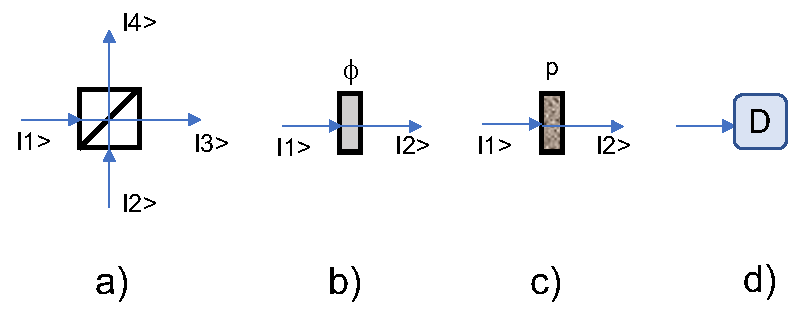
\includegraphics[scale=0.9]{Pictures/Fig-Optique.pdf} 
\end{center}
\caption{Elements optiques: a) séparateur de faisceau 50/50; b) lame de phase; c) lame absorbante ; d) détecteur.}
\label{fig:Optique}
\end{figure}

La figure \ref{fig:Optique} réprésente 4 éléments optiques.

Le panneau a) représente un séparateur de faisceau 50/50. Les ports d'entrée et de sortie sont notés 1,2 et 3,4 respectivement. Si un photon entre par le port 1, ou par le le port 2, il subit la transformation
\begin{eqnarray}
\vert 1 \rangle &\to & \frac{1}{\sqrt{2}} \vert 3 \rangle + \frac{i}{\sqrt{2}} \vert 4 \rangle \\
\vert 2 \rangle &\to & \frac{i}{\sqrt{2}} \vert 3 \rangle + \frac{1}{\sqrt{2}} \vert 4 \rangle 
\end{eqnarray}
(noter les facteur $i$ qui rendent cette transformation unitaire).

Le panneau b) représente une lame de phase qui réalise la transformation
\begin{eqnarray}
\vert 1 \rangle &\to & e^{i \phi}  \vert 2 \rangle \ .
\label{Eq:opt3}
\end{eqnarray}

Le panneau c) représente une lame absorbante. Cette lame absorbe le photon avec une probabilité $p$ et laisse passer le photon avec une probabilité $1-p$. Nous pouvons modéliser la lame absorbante par la transformation
\begin{eqnarray}
\vert 1 \rangle &\to & \sqrt{p}  \vert ABS \rangle + \sqrt{1-p}  \vert 2 \rangle 
\end{eqnarray}
ou $\vert ABS \rangle$ représente l'état si le photon est absorbé, et $\vert 2 \rangle $ représente le photon si il a traversé la lame sans être absorbé.

d) représente un détecteur de photon unique.



\begin{figure}[h!]
\begin{center}
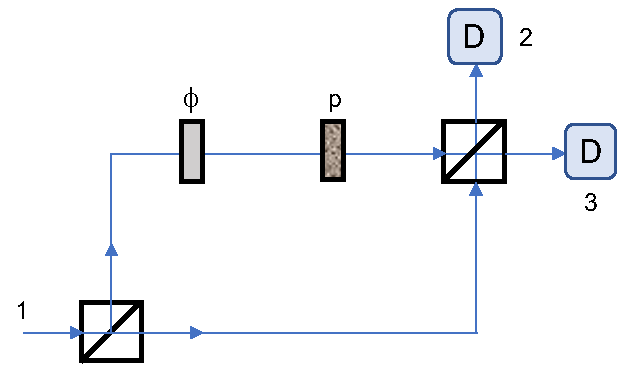
\includegraphics[width=0.5\columnwidth]{Pictures/Fig-Interf.pdf} 
\end{center}
\caption{Interférometre de Mach-Zehnder dans un bras duquel on a mis une lame de phase et une lame absorbante.}
\label{fig:MZ}
\end{figure}


La figure \ref{fig:MZ} représente un interférometre de Mach-Zehnder dans un bras duquel on a mis une lame de phase et une lame absorbante.  Le port d'entrée du photon est noté $1$, et les deux ports de sortie $2$ et $3$.

\begin{enumerate}
\item Expliquer pourquoi, si la probabilité que la lame absorbante absorbe le photon est $p$, l'équation \eqref{Eq:opt3} qui permet de décrire son action sur un photon contiens des facteurs $\sqrt{p}$ et $\sqrt{1-p}$. Pourquoi ces racines carrées?

\item 
Supposons qu'un photon entre par le port $1$ de l'interférometre de la figure \ref{fig:MZ}. L'état final du photon peut s'écrire comme une combinaison linéaire des états $ \vert ABS \rangle $, $ \vert 2 \rangle $ et $ \vert 3 \rangle $. Donner cet état final en fonction de $\phi$ et $p$.

\item Donner la probabilité de trouver le photon dans les ports $2$ et $3$ de l'interférometre en  fonction de $\phi$ et $p$.

\item Pour $p$ donné, quel est la valeur minimale de trouver le photon dans le port $2$ (lorsqu'on varie $\phi$).

\item Représenter dans un graphique la probabilité de trouver le photon dans le port 2 en fonction de $\phi$, lorsque $p=1/3$. (Utiliser la page quadrillée).


\end{enumerate}

%\begin{center}
%\begin{tikzpicture}
%\def\sizx{15};
%\def\sizy{22};
%\draw[help lines, step = 0.5cm] (0,0) grid (\sizx, \sizy);
%\end{tikzpicture}
%\end{center}

\chapter{Juin 2022}

\paragraph{Question 1} \textit{Spin 1/2.} \\

Soit un spin  1/2 dont l'état à l'instant $t=0$ est
\begin{equation}
\vert \psi \rangle =  \frac{1}{2} \lvert \uparrow \rangle + 
 \frac{\sqrt{3} }{2} \lvert \downarrow \rangle
\end{equation}
(avec $\lvert \uparrow \rangle$, 
$\lvert \downarrow \rangle$ les états propres de $\sigma_z$).

Ce spin évolue avec un Hamiltonien donné par 
\begin{equation}
H = \frac{\hbar \omega }{2}\sigma_z\ .
\end{equation}

\begin{enumerate}
\item 
A l'instant $t=0$ on mesure les opérateurs $\sigma_x$, $\sigma_y$ ou $\sigma_z$.
Quelles sont les valeurs moyennes
\begin{eqnarray}
\langle \psi \rvert \sigma_x \lvert \psi \rangle &=& ?\nonumber\\
\langle \psi \rvert \sigma_y \lvert \psi \rangle &=& ?\nonumber\\
\langle \psi \rvert \sigma_z \lvert \psi \rangle &=& ?\nonumber
\end{eqnarray}

\item

Quel est l'état à l'instant $t$ ?

\item

Quelle est est la valeur moyenne de $\sigma_x$  à l'instant $t$ ?
\begin{eqnarray}
\langle \psi (t)\rvert \sigma_x \lvert \psi (t)\rangle &=& ?\nonumber
\end{eqnarray}

\item 
A l'instant $t$ on mesure l'opérateur $\sigma_x$. Quelle est la probabilité de trouver le résultat $+x$ en fonction de $t$?

\end{enumerate}

\paragraph{Question 2} \textit{L'opérateur $\hat S(\beta)$.} \\

Les opérateurs sans dimension position $\hat x$ et impulsion $\hat p$ satisfont 
\begin{equation}
[\hat x, \hat p ] = i\ .
\label{xp:1}
\end{equation}

Nous noterons $\lvert x \rangle$ et $\lvert p \rangle$ les états propres de $\hat x$ et de $\hat p $ respectivement, pour tout $x, p \in \mathbb{R}$.

Considérons la famille d'opérateurs
\begin{equation}
\hat S(\beta) = \exp \left( -i \beta \hat x \right)\quad , \quad \beta \in \mathbb{R}\ .
\end{equation}




\begin{enumerate}


\item 
Montrer que $\hat S(\beta_1) \hat S(\beta_2)=\hat S(\beta_1 + \beta_2) $. 

\item
Que vaut le commutateur $[ \hat x,  \hat S(\beta)]$ ?

\item
Montrer que $[ \hat p,  \hat S(\beta)] = - \beta \hat S(\beta)$.


\item
Que vaut $\langle x' \rvert S(\beta) \lvert x \rangle$ ?

\item
Montrer que $\hat S(\beta) \lvert p \rangle$ est un état propre de $\hat p$, et déterminer sa valeur propre.

\item Soit l'état qui en représentation position s'écrit $\lvert \psi\rangle = c\int dx\ \exp (-x^2 + i 3 x)\lvert x \rangle$  avec $c$ une constante de normalisation.

Quelle est la fonction d'onde en représentation position de 
$\hat S(\beta) \lvert \psi\rangle $ ?


\end{enumerate}


\paragraph{Question 3} \textit{Pegg--Barnett phase states.} \\




{\bf Rappels et définitions}

 En unités sans dimensions ($\hbar=1$), les opérateurs position $\hat x$ et impulsion $\hat p$ obéissent à la relation de commutation canonique $[\hat x, \hat p]=i $.  Les opérateurs de création et destruction sont définis par 
$\hat a= \frac{1}{\sqrt{2}}(\hat x+i\hat p)$, $a^\dagger= \frac{1}{\sqrt{2}}(\hat x-i\hat p)$ et satisfont donc $[\hat a,\hat a^\dagger]=1$. L'opérateur nombre $\hat n$ est donné par $\hat n= \hat a^\dagger \hat a$ et ses vecteurs propres sont notés $\hat n \ket{n} =n \ket{n}$ où $n \in \mathbb{N}$. 
%On peut montrer que $\hat a \ket{n} =\sqrt{n} \ket{n-1}$ et que $\hat a^\dagger \ket{n} =\sqrt{n+1} \ket{n+1}$. 
L'hamiltonien de l'oscillateur harmonique est $\hat H = \frac{1}{2}\omega ( \hat P^2 + \hat X^2 ) = \omega (\hat n + 1/2)\ $. \\



Nous noterons ${\cal H}^{(N)}={\text{span}}\{\lvert 0\rangle, \dotsc, \lvert N-1\rangle\}$ l'espace de Hilbert de dimension $N$ dont une base est constituée des états 
$\lvert 0\rangle, \dotsc, \lvert N-1\rangle$ (les $N$ premiers états nombre)
%, et   ${\cal H}={\mathrm span}\{\vert n\rangle, \ n\in \mathbb{N}\}$ l'espace infini dimensionel de Hilbert de l'oscillateur harmonique.
et $\mathbb{I}^{(N)} =\sum_{n=0}^{N-1} \lvert n \rangle \langle n \rvert$ l'opérateur identité sur ${\cal H}^{(N)}$.


Pour chaque valeur de $N\in \mathbb{N}$, définissons les $N$ états
\begin{equation}
\lvert \psi^{(N)}_m\rangle = \frac{1}{\sqrt{N}} \sum_{n=0}^{N-1} e^{\frac{i 2 \pi  nm}{N}} \lvert n \rangle\quad , \quad m=0,1,\dotsc,N-1\ .
\label{eq:states}
\end{equation}
Ces états ont été introduits par Pegg et Barnett en 1988, et s'appellent les ``Pegg-Barnett phase states''.

Nous allons montrer que pour chaque valeur de $N$ ces états constituent une base orthonormée de ${\cal H}^{(N)}$ (Questions \ref{poin3} et \ref{poin4}), et que ces états évoluent cycliquement entre eux sous l'action de l'Hamiltonien de l'oscillateur harmonique (Question \ref{poin5}).


Nous aurons besoin de la somme 
\begin{equation}
\sum_{k=0}^{N-1} e^{\frac{i 2 \pi  k l}{N}}=N\delta_{l,0} \quad , \quad N\in \mathbb{N}  \quad , \quad  l=0,1,\dotsc,N-1\ .\\
\label{eq:sum}
\end{equation}


{\bf Questions.}

\begin{enumerate}



\item

Ecrivez explicitement les 4 états $\lvert \psi^{(4)}_m\rangle$, $m=0,1,2,3$.


\item


Soit $\hat H$  l'Hamiltonien de l'oscillateur harmonique.

Ecrire dans la base nombre l'état $\lvert \psi^{(N)}_m\rangle$ ayant évolué pendant un temps $t$:
\begin{equation}
e^{-i t \hat H} \lvert \psi^{(N)}_m\rangle
\end{equation}

\item
\label{poin5}

Utilisez la réponse à la question précédente pour montrer que pour certains intervalles de temps discrets ($t={\frac{ 2 \pi k}{N \omega}}$ avec $k$ entier) les états $\lvert \psi^{(N)}_m\rangle$ se transforment entre eux:
\begin{equation}
e^{-i \frac{ 2 \pi k}{N \omega}\hat H} \lvert \psi^{(N)}_m\rangle = e^{i\varphi}
\lvert \psi^{(N)}_{{m - k} \mod N}\rangle
 \quad , \quad  \forall k\in \{0,1,\dotsc,N-1\}
\ . \label{eq:evol}
\end{equation}
et donnez la phase $\varphi$ dans \eqref{eq:evol}.

\item 

Montrez l'égalité des membres de gauche et de droite de l'équation \eqref{eq:sum} dans le cas $l=0$.

(Si vous savez le faire, démontrez la relation \eqref{eq:sum}  pour $l\neq 0$).

\item
\label{poin3}

Montrez (en utilisant \eqref{eq:sum}) que pour $N$ fixé, les états $\lvert \psi^{(N)}_m\rangle$ sont orthonormés:
\begin{equation}
\langle \psi^{(N)}_{m'} \vert \psi^{(N)}_m\rangle = \delta_{m' m}\ .
\end{equation}

\item
\label{poin4}

Montrez  (en utilisant \eqref{eq:sum})  que, pour $N$ fixé, la somme des projecteurs sur les états 
$\lvert \psi^{(N)}_m\rangle$  est l'opérateur identité sur ${\cal H}^{(N)}$:
\begin{equation}
\sum_{m=0}^{N-1} \lvert  \psi^{(N)}_{m} \rangle \langle \psi^{(N)}_m\rvert = \mathbb{I}^{(N)}\ .
\end{equation}


\end{enumerate}

\chapter{Août 2022}

\paragraph{Question 1.} \textit{Oscillateur Harmonique.}\\

En unités sans dimensions ($\hbar=1$), les opérateurs position $\hat x$ et impulsion $\hat p$ obéissent à la relation de commutation canonique $[\hat x, \hat p]=i $.  Nous noterons $\lvert x \rangle$ et $\lvert p \rangle$ les états propres de $\hat x$ et de $\hat p $ respectivement, pour tout $x, p \in \mathbb{R}$.

Les opérateurs de création et destruction sont définis par 
$\hat a= \frac{1}{\sqrt{2}}(\hat x+i\hat p)$, $a^\dagger= \frac{1}{\sqrt{2}}(\hat x-i\hat p)$ et satisfont donc $[\hat a,\hat a^\dagger]=1$. L'opérateur nombre $\hat n$ est donné par $\hat n= \hat a^\dagger \hat a$ et ses vecteurs propres sont notés $\hat n \ket{n} =n \ket{n}$ où $n \in \mathbb{N}$. 

L'hamiltonien de l'oscillateur harmonique est $\hat H = \frac{1}{2}\omega ( \hat P^2 + \hat X^2 ) = \omega (\hat n + 1/2)\ $. \\

Soit l'état $\vert \psi \rangle$ qui dans la base nombre s'écrit
\begin{equation}
\vert \psi \rangle = \alpha \vert n \rangle + \beta \vert n+1 \rangle 
\end{equation}
avec $n\geq 0$ un entier, et $\alpha,\beta \in \mathbb{C}$ deux nombres complexes satisfaisant $\vert \alpha \vert^2 + \vert \beta \vert^2=1$.

\begin{enumerate}
\item 
Donnez la forme des états $a \vert \psi \rangle$ et $a^\dagger \vert \psi \rangle$ (dans la base nombre).
\item
Que valent les valeurs moyennes\\
de $\hat x$, \\
de $\hat p$, \\
de $\hat x^2$\\
dans l'état $\vert \psi \rangle$ ?

\end{enumerate}
Donnez les réponses 
en fonction de $\alpha, \beta, n$. N'oubliez pas que $\alpha$ et $\beta$ sont complexes.

\paragraph{Question 2.} \textit{Photon se propageant dans un millieu optiquement actif.} \\






Le nombre d'onde $k$ d'un photon de fréquence angulaire $\omega$ se propageant dans un milieu d'indice de réfraction $n$ est donné par
\begin{equation}
k= \frac{n \omega}{c} 
\end{equation}
avec $c$ la vitesse de la lumière dans le vide.
La fonction d'onde d'un tel photon se propageant dans la direction des z positifs est donnée par
\begin{equation}
\psi(t,z) = A e^{-i \omega t} e^{i k z}\ .
\end{equation}


La polarisation d'un photon est décrit par un espace de Hilbert ${\cal H}_{pol}$ de dimension 2.

Nous noterons $\vert V\rangle$ et $\vert H\rangle$ les états correspondant à un photon polarisé verticalement et horizontalement. Ces deux états constituent une base orthonormée de l'espace de Hilbert ${\cal H}_{pol}$ .

Un photon dans un état de polarisation linéaire, à un angle $\theta$ de la verticale ($\theta \in [0,\pi/2[$) est dans l'état 
\begin{equation}
\vert \theta \rangle = \cos \theta \vert V\rangle + \sin \theta \vert H\rangle\ .
\label{eq:theta}
\end{equation}

Un polariseur orienté selon l'axe $\theta$ laissera passer la lumière dans l'état 
$\vert \theta \rangle$ et absorbera la lumière dans l'état $\vert \theta + \pi/2 \rangle$. Il peut donc être vu comme un système de mesure quantique qui mesure dans la base $\vert \theta \rangle$ et $\vert \theta +\pi/2 \rangle$


Nous pouvons également utiliser la base de polarisation circulaire droite et gauche donnée par 
\begin{eqnarray}
\vert D \rangle &=& \frac{1}{\sqrt{2}} \vert V\rangle + \frac{i}{\sqrt{2}} \vert H\rangle\nonumber\\
\vert G \rangle &=& \frac{1}{\sqrt{2}} \vert V\rangle - \frac{i}{\sqrt{2}} \vert H\rangle\ .
\end{eqnarray}



Certaines molécules sont chirales: il existe deux formes distinctes (appelés énantiomères) de la molécule qui sont image miroir l'une de l'autre. De nombreuses molécules organiques (par exemple des sucres, des acides animés) sont des molécules chirales. Généralement les être vivants utilisent un seul des énantiomères, mais pas l'autre. Par exemple l'isomère D du glucose, appelé dextrose, est très répandu dans le milieu naturel, mais pas l'isomère L.

Si un liquide (par exemple de l'eau) contient en solution une plus grande quantité d'un énantiomère d'une molécule chirale, il devient optiquement actif. Par exemple de l'eau avec du dextrose dissout est optiquement actif.

Dans un milieu optiquement actif, lles polarisations gauche et droite percoivent des indices de réfraction différents, notés $n_G$ et $n_D$.
La fonction d'onde d'un photon de polarisation gauche ou droite est donc donnée par
\begin{eqnarray}
\vert \psi_G(t,z)\rangle  = \exp \left( -i \omega t + i \frac{n_G \omega}{c} z\right) \vert G\rangle  \ , \nonumber\\
 \vert  \psi_D(t,z)  \rangle =  \exp \left(  -i \omega t + i \frac{n_D \omega}{c} z \right) \vert D\rangle \  .
 \label{eq:psiGD}
\end{eqnarray}




\begin{figure}
\centering
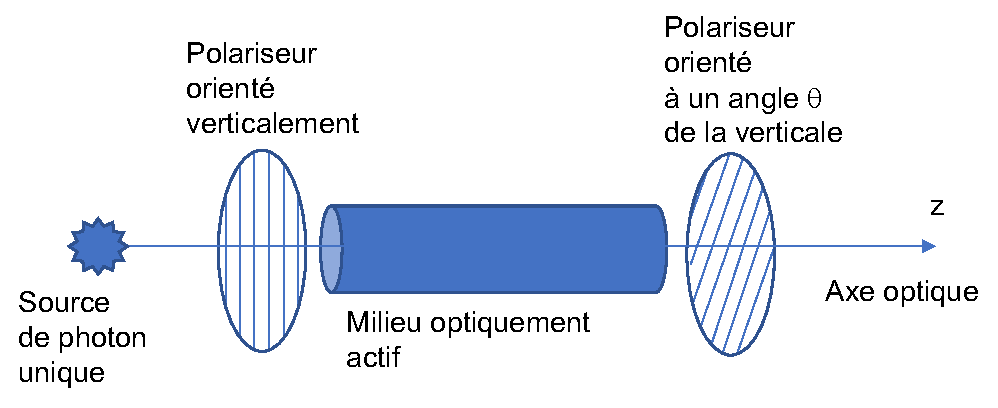
\includegraphics[scale=0.8]{Pictures/Fig-Pol.pdf}
\end{figure}

Nous considérons le dispositif illustré dans la figure consititué d'une source de photon unique, d'un polariseur, d'un tube de longueur $L$ contenant un liquide optiquement actif. Le tube est suivi d'un second polariseur dont on peut faire tourner l'orientation pour analyser la polarisation après passage dans le liquide.

Si le photon traverse le premier polariseur il est dans l'état $\vert V \rangle$.

Montrer qu'à la sortie du tube contenant le liquide optiquement actif, le photon est dans un état de polarisation linéaire selon la direction $\theta = \frac{(n_G - n_D) \omega L}{2 c}$.
(Pour cela nous recommandons d'exprimer l'état $\vert V \rangle$ à la sortie du polariseur dans la base $\vert G\rangle, \vert D \rangle$; d'utiliser l'équation \eqref{eq:psiGD} pour obtenir l'état à la sortie du liquide; de repasser dans la base $\vert H\rangle, \vert V \rangle$; et puis de comparer l'état ainsi obtenu avec l'équation \eqref{eq:theta}).





\paragraph{Question 3.} \textit{Etat propre de l'Hamiltonien d'énergie nulle.} \\

\begin{figure}
\centering
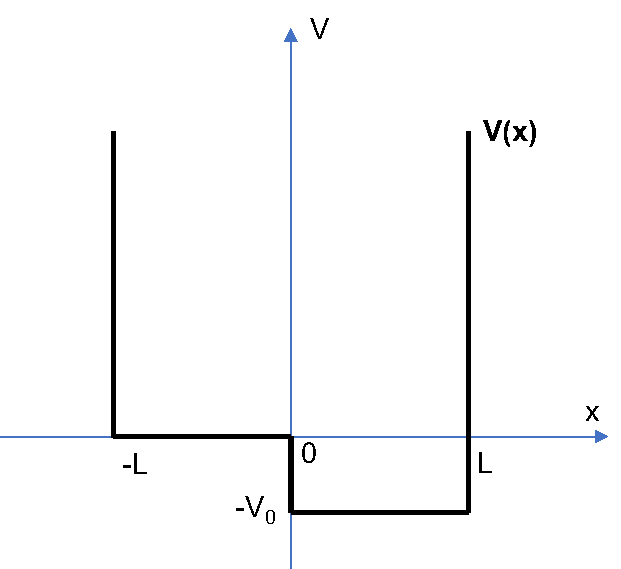
\includegraphics[scale=0.8]{Pictures/FigPot.pdf}
\end{figure}


Considérons une particule de masse $m$ se déplacant dans un potentiel à une dimension $V(x)$. Les états propres de l'hamiltonien satisfont  à l'équation
\begin{equation}
E \psi(x) = - \frac{\hbar^2}{2 m} \partial_x^2 \psi(x) + V(x) \psi(x)
\end{equation}

Le potentiel a
la forme suivante (voir figure):
\begin{eqnarray}
V(x)=+\infty &\quad , \quad& x<-L\nonumber\\
V(x)=0 &\quad , \quad& -L\leq x < 0 \nonumber\\
V(x)=-V_0 &\quad , \quad& 0 \leq x < L \nonumber\\
V(x)=+\infty &\quad , \quad& L\leq x \ .
\end{eqnarray}

Nous supposerons que $L$ est fixé, mais que $V_0>0$ est un paramètre qui peut être ajusté expérimentalement.

Nous cherchons à déterminer les valeurs de $V_0$ telles que l'hamiltonien ait une état propre d'énergie $E=0$.

\newpage

\begin{enumerate}
\item
En supposant $E=0$, écrire les équations auxquelles doit satisfaire $\psi(x)$ dans les différentes régions de l'espace.

\item
Donner les conditions au bord (en $x=-L$ et $x=+L$) et les conditions de raccord là ou le potentiel est discontinu (en $x=0$).

\item
Résoudre ces équations et obtenir une équation implicite pour $V_0$ telle que l'hamiltonien ait un été lié d'énergie $E=0$.
\item

Les deux premières solutions de $$z+ \tan z =0$$ 
(pour $z\geq 0$) sont
$z=0$ et $z=2.03$. Utilisez cette information pour déterminer la  plus petite valeur de $V_0$ telle que l'hamiltonien ait un été lié d'énergie $E=0$.


\end{enumerate}

\end{document}